\documentclass[12pt,a4paper]{report}
% \bibliographystyle{abbrv}
\usepackage{graphicx}
\usepackage{tabularx,adjustbox}
\usepackage{subfig}
\usepackage{xtab}
\usepackage{longtable}
\usepackage{tablefootnote}
\usepackage{subcaption}
\usepackage{adjustbox,makecell, cellspace}
\usepackage{soul}
\usepackage{threeparttable}
\usepackage{multirow}
\usepackage{mathtools}
\usepackage{float}
\pagestyle{plain}
\usepackage{siunitx}
\newcolumntype{P}[1]{>{\centering\arraybackslash}p{#1}}
\usepackage{csquotes}
\usepackage{amsmath,amssymb,amsfonts}
\usepackage{algcompatible}
\usepackage{multirow}
\usepackage[acronym]{glossaries}
\usepackage[labelsep=period]{caption}
\captionsetup[table]{name=TABLE,labelsep=newline}
\usepackage{booktabs,caption}
\usepackage{enumerate}
\usepackage{graphicx}
\usepackage{environ}
\NewEnviron{myequation}{%
    \begin{equation}
    \scalebox{1.1}{$\BODY$}
    \end{equation}}
\usepackage{tablefootnote}
\usepackage{colortbl}
\usepackage{float}
\usepackage{algpseudocode}
\usepackage{algorithm}
\usepackage{alphalph,array}
\usepackage{subfig}
\renewcommand\thesubfigure{\alphalph{\value{subfigure}}}
\usepackage[fit]{truncate}
\usepackage{fancyhdr}
%\usepackage{apacite}
\pagestyle{fancy}
\fancyhf{}
\fancyhead[R]{\fontsize{8}{8}\selectfont\itshape\nouppercase{\textcolor{internationalkleinblue}\leftmark}}
\fancyfoot[R]{\fontsize{8}{8}\selectfont\itshape\nouppercase{\thepage}}
\fancyfoot[C]{\fontsize{7}{7}\selectfont\itshape\nouppercase{\textcolor{internationalkleinblue}{SleepGCN-Transformer: A Hybrid Graph
Convolutional and Transformer Network for Sleep
Stage Classification
}}}
\fancyfoot[L]{\fontsize{8}{8}\selectfont\itshape\nouppercase{\textcolor{internationalkleinblue}{PDEU}}}
\footrule{\footskip=1.7pt}
\makeatletter
\def\footrule{{\color{auburn}\if@fancyplain\let\footrulewidth\plainfootrulewidth\fi
		\hrule\@height 2pt\@width\headwidth\vskip 1pt
		\hrule\@height\headrulewidth\@width\headwidth \footskip \dimexpr-\footrulewidth-0.5pt\relax}}
\def\headrule{\color{auburn}{\if@fancyplain\let\headrulewidth\plainheadrulewidth\fi
		\hrule\@height 2pt\@width\headwidth\vskip 1pt
		\hrule\@height\headrulewidth\@width\headwidth \vskip\dimexpr-\headrulewidth-2pt\relax}}
\makeatother 

\usepackage{setspace}
% \usepackage[round]{natbib}
\usepackage[sort, numbers]{natbib}
\usepackage{hyperref}
\usepackage{epstopdf}
\usepackage{amsmath}
\usepackage{pdfpages}
\usepackage{chngcntr}
\usepackage[english]{babel}
\usepackage{blindtext}
\usepackage{mathptmx}% Times Roman font
\usepackage[scaled=.90]{helvet}
\usepackage[toc,page]{appendix}
\usepackage{subfig}
\usepackage{pifont}% http://ctan.org/pkg/pifont
\usepackage{csquotes}
\usepackage{amsmath,amssymb,amsfonts}
\usepackage[acronym]{glossaries}
\usepackage[toc,page]{appendix}
\usepackage{xcolor,sectsty}
\definecolor{auburn}{rgb}{0.43, 0.21, 0.1}
\definecolor{vividauburn}{rgb}{0.58, 0.15, 0.14}
\definecolor{bole}{rgb}{0.47, 0.27, 0.23}
\definecolor{royalblue(traditional)}{rgb}{0.0, 0.14, 0.4}
\definecolor{midnightblue}{rgb}{0.1, 0.1, 0.44}
\definecolor{internationalkleinblue}{rgb}{0.0, 0.18, 0.65}
\definecolor{bondiblue}{rgb}{0.0, 0.58, 0.71}
\definecolor{magicmint}{rgb}{0.67, 0.94, 0.82}
\definecolor{cadmiumgreen}{rgb}{0.0, 0.42, 0.24}
\definecolor{LightCyan}{rgb}{0.88,1,1}
\definecolor{gainsboro}{rgb}{0.86, 0.86, 0.86}
\definecolor{LightCyan}{rgb}{0.80,1,1}
\definecolor{amber}{rgb}{1.0, 0.88, 0.0}	
\definecolor{Gray}{gray}{0.9}
\definecolor{amethyst}{rgb}{0.6, 0.6, 0.8}
\definecolor{inchworm}{rgb}{0.7, 0.93, 0.36}
\definecolor{cherryblossompink}{rgb}{0.98, 0.8, 0.91}
\definecolor{electriclime}{rgb}{0.8, 1.0, 0.0}
\definecolor{lavenderblue}{rgb}{0.8, 0.8, 1.0}
\definecolor{atomictangerine}{rgb}{1.0, 0.7, 0.0}
\definecolor{atomictangerine1}{rgb}{1.0, 0.64, 0.26}
\definecolor{capri}{rgb}{0.0, 0.75, 1.0}
\definecolor{LightCyan}{rgb}{0.80,1,1}
\definecolor{amber}{rgb}{1.0, 0.88, 0.0}	
\definecolor{Gray}{gray}{0.9}
\definecolor{amethyst}{rgb}{0.6, 0.6, 0.8}
\definecolor{lavendergray}{rgb}{0.77, 0.76, 0.82}
\definecolor{bleudefrance}{rgb}{0.19, 0.55, 0.90}
\definecolor{amethyst}{rgb}{1, 0.4, 0.8}
\definecolor{brilliantlavender}{rgb}{0.96, 0.73, 1.0}
\definecolor{cadmiumyellow}{rgb}{1.0, 0.96, 0.0}
\definecolor{chartreuse(web)}{rgb}{0.5, 1.0, 0.0}
\definecolor{electricgreen}{rgb}{0.0, 1.0, 0.0}
\definecolor{pear}{rgb}{0.82, 0.89, 0.19}
\definecolor{bananamania}{rgb}{0.98, 0.91, 0.71}
\definecolor{babyblue}{rgb}{0.54, 0.81, 0.94}
\definecolor{celadon}{rgb}{0.67, 0.88, 0.69}
\usepackage{caption}
\DeclareCaptionFont{royalblue(traditional)}{\color{royalblue(traditional)}}
\captionsetup[figure]{labelfont=royalblue(traditional),textfont=royalblue(traditional)}
\captionsetup[table]{labelfont={color=midnightblue},font={color=midnightblue}}
\usepackage{titlesec}
\titleformat{\chapter}[display]
{\huge\bfseries\color{auburn}}
{\chaptertitlename\ \thechapter}{15pt}{\Huge}
\titleformat{\section}
{\Large\bfseries\color{vividauburn}}
{\thesection}{12pt}{}
\subsectionfont{\color{bole}} 
\usepackage{setspace}
\doublespacing
\usepackage{xpatch}
\makeatletter

\xpatchcmd{\@chapter}{%
	\ifnum \c@secnumdepth >\m@ne
	\refstepcounter{chapter}%
	\typeout{\@chapapp\space\thechapter.}%
	\addcontentsline{toc}{chapter}%
	{\protect\numberline{\thechapter}#1}%
	\else
	\addcontentsline{toc}{chapter}{#1}%
	\fi
}{%
\ifnum \c@secnumdepth >\m@ne
\refstepcounter{chapter}%
\typeout{\@chapapp\space\thechapter.}%
\addcontentsline{toc}{chapter}%
{\protect\numberline{\thechapter}\protect\parbox[t]{0.9\linewidth}{#2}}%
\else
\addcontentsline{toc}{chapter}{\protect\parbox[t]{0.9\linewidth}{#2}}%
\fi
\addtocontents{toc}{\protect\addvspace{0.5\baselineskip}}% Some spacing afterwards
}{}{}

\makeatother
\usepackage{blindtext}
\usepackage{hyperref}
\hypersetup{colorlinks,citecolor=black,filecolor=black,linkcolor=black,urlcolor=black}














\begin{document}
	\pagestyle{plain}\clearpage
        \thispagestyle{empty}
	\begin{center}
    {{\Large \textbf{SleepGCN-Transformer: A Hybrid Graph Convolutional and
Transformer Network for Sleep Stage Classification
}}}\\
    \vspace{0.6cm}
    {\large A Master's Report}\\
    {\large Submitted in partial fulfillment of the requirement for the award of the degree of}\\
    \vspace{0.8cm}
    {\large Master of Technology in Artificial Intelligence}\\
    {\large by}\\
    \textbf{{\Large  Tanmay Rathod}}\\
    {\large 23MAI007}\\
    \vspace{0.7cm}
    {\large Under the guidance of}\\
    {\large  \textbf{Dr. Santosh Kumar Satapathy}  {\large }}\\
    {\large Department of Information and Communication Technology}\\
    \vspace{0.6cm}
        \vfill
    {\centering 
\includegraphics[width=0.21\textwidth]{img/pdpu_logo.png}}\\
    {\large School of Technology}\\
    {\large Pandit Deendayal Energy University}\\
    {\large Gandhinagar – 382426. Gujarat - India}\\
    {\large February, 2025}
\end{center}
		\begin{center}
	\textbf{\large Student Declaration}
\end{center}

I, \textcolor{internationalkleinblue}{\textbf{Tanmay Rathod}}, hereby declare that this written submission represents my ideas in my own words, and  where others’ ideas or words have been included, I have adequately cited and referenced the original sources. I also declare that I have adhered to all principles of academic honesty and integrity and have not misrepresented or fabricated, or falsified any idea/data/fact/source in my submission. I understand that any violation of the above will be cause for disciplinary action by the Pandit Deendayal Energy University and can also evoke penal action from the sources which have thus not been properly cited or from whom proper permission has not been taken when needed.
\vspace{0.8cm}
\vspace{0.8cm}
\begin{flushright}
    \makebox[1.8in]{\hrulefill}\\
    Tanmay Rathod\\
    Roll No: 23MAI007\\
\end{flushright}
\vfill
\begin{flushleft}
	Date: \makebox[1.8in]{\hrulefill}
\end{flushleft} 
	% \includepdf[pages={1}]{Charul 3rd.pdf}
	\thispagestyle{empty}

         \pagestyle{plain}\clearpage
        \thispagestyle{empty}
	\begin{center}
	\textbf{\large Approval Sheet}
\end{center}

This thesis entitled \textbf{\enquote{SleepGCN-Transformer: A Hybrid Graph Convolutional and Transformer Network for Sleep Stage Classification}} by \textbf{Tanmay Rathod} is recommended for the degree of \textbf{M.Tech} in \textbf{Artificial Intelligence}.

\vspace{1cm}

\begin{table}[h!]
	\centering
	\begin{tabular}{@{}m{0.45\textwidth}<{\centering} m{0.45\textwidth}<{\centering}@{}}
		\textbf{Expert 1} & \textbf{Expert 2} \\[2.5em]
		\rule{0.35\textwidth}{0.4pt} & \rule{0.35\textwidth}{0.4pt} \\[0.5em]
		Mr. Nilesh Ranpura & Dr. Hridoy Sankar Dutta \\[0.5em]
		Director of Engineering, & Lecturer (Assistant Professor), \\[0.5em]
		Arrow Inc. (E-Infochips) & Deakin University \\[3em]
	\end{tabular}
\end{table}

\begin{table}[h!]
	\centering
	\begin{tabular}{@{}m{0.31\textwidth}<{\centering} m{0.31\textwidth}<{\centering} m{0.31\textwidth}<{\centering}@{}}
		\textbf{Guide} & \textbf{Head of Department} & \textbf{Director} \\[2.5em]
		\rule{0.25\textwidth}{0.4pt} & \rule{0.25\textwidth}{0.4pt} & \rule{0.25\textwidth}{0.4pt} \\[0.5em]
		Dr. Santosh Satapathy & Dr. Paawan Sharma & Prof.(Dr.) Dhaval Pujara \\[0.5em]
		Assistant Professor, & HoD, Dept. of ICT, & Director, \\[0.5em]
		Dept. of ICT & School of Technology & School of Technology \\
	\end{tabular}
\end{table}

\vfill
\begin{flushleft}
	Date: \makebox[1.8in]{\hrulefill}\\
	Place: \makebox[1.8in]{\hrulefill}\\    
\end{flushleft}

      



        \pagenumbering{roman}
        \section*{\textcolor{internationalkleinblue}{\textbf{Acknowledgment}}}

Although this thesis bears only my name as the author, its successful completion is the result of the support, guidance, and encouragement of several individuals to whom I am deeply grateful.

First and foremost, I would like to express my sincere gratitude to my internal guide, Dr. Santosh Kumar Satapathy, from Pandit Deendayal Energy University (PDEU), for his unwavering support throughout the course of this project. His valuable insights, constructive feedback, and continuous encouragement were instrumental in shaping the direction of this research and overcoming various challenges.

I also acknowledge the faculty members and staff of the M.Tech in Artificial Intelligence program at PDEU for providing a stimulating academic environment and the foundational knowledge that enabled me to undertake this work.

Finally, I extend heartfelt thanks to my family and friends for their constant encouragement, patience, and moral support throughout this journey.

This thesis would not have been possible without the collective contributions of these individuals, and I remain truly thankful to all.

\begin{flushright}
	\textbf{Tanmay Rathod}\\
\end{flushright}

	\thispagestyle{empty}
	\begin{center}
% 	{{\Large \textbf{Dedicated to}}}\\
% 	\vspace{0.8cm}
% {\large \textit{\textbf{Grand Father and Grand Mother}... You lightened it }}\\
% {\large \textit{\textbf{Papa}...You envisioned this.}}\\ 
% {\large \textit{Your determination and belief made this a reality..}}\\
% \vspace{0.5cm}
% {\large \textit{\textbf{Mummy}...Your faith and prayers have lead us here..}}\\
% {\large \textit{Your patience \& support made this a reality..}}\\
% \vspace{0.5cm}
% {\large \textit{\textbf{Jagruti \& Hetal \& Aarush}.. You made me laugh at the lowest points..}}
% {\large \textit{You made me believe that I can..}}\\

\end{center}
	\clearpage\thispagestyle{empty}

\clearpage\thispagestyle{empty}

 
	\begin{center}
\section*{\textcolor{internationalkleinblue}{\textbf{{Abstract}}}}
\end{center} 
This project presents \textit{SleepGCN-Transformer}, a hybrid model combining Graph Convolutional Networks (GCN) and Transformer encoders for sleep stage classification. Using the SleepEDF dataset, it incorporates four physiological signals: EEG (Fpz-Cz, Pz-Oz), EMG (submental), and EOG (horizontal). Preprocessing includes 30-second epochs, band-pass filtering (0.3--30 Hz), and graph-based EEG channel representation.

The GCN module captures spatial relationships across EEG channels, while the Transformer encoder models temporal dependencies from graph-level embeddings. Focal Loss addresses class imbalances, and a CosineAnnealingLR scheduler optimizes learning rate decay. Training with the AdamW optimizer for 20 epochs achieves 93.12 \% training and 93.04\% validation accuracy.

Model performance, assessed using precision, recall, and F1-score, demonstrates high efficacy. LIME-based feature importance analysis highlights EMG and EEG Pz-Oz channels as key contributors. This hybrid model exhibits state-of-the-art performance, with future directions focused on enhancing explainability and clinical integration.
	\thispagestyle{empty}
	
        \addcontentsline{toc}{chapter}{Contents}	\tableofcontents
	\addcontentsline{toc}{chapter}{List of Figures}
	\listoffigures
	\addcontentsline{toc}{chapter}{List of Tables}
	\listoftables
 
    
	\cleardoublepage\pagenumbering{arabic}
	\pagestyle{fancy}


\chapter{Introduction}
\label{chapter1}
Sleep is a fundamental aspect of human health that greatly contributes to cognitive function, memory consolidation, and emotional regulation. Proper and quality sleep guarantees proper brain function and overall physical and mental health. Sleep disturbances result in several diseases, such as impaired concentration, mood disorders, and chronic conditions like cardiovascular diseases.

Sleep plays a critical function in sustaining physical and mental well-being. It is not a passive resting state but a sophisticated biological process crucial for memory consolidation, emotional homeostasis, metabolic health, and immune system function. Alterations in sleep quality or sleep patterns can reflect or lead to many health problems, such as insomnia, depression, cardiovascular disease, and neurodegenerative disorders. It is essential for clinicians and scientists to precisely assess sleep stages for the diagnosis of such conditions and the prescription of proper treatment plans.


Staging of the sleep stages is the basis of understanding the architecture of sleep and the diagnosis of sleep disorders. Sleep is divided into five major stages—N1, N2, N3, REM, and Wake—based on unique patterns seen in brain function. Every stage of sleep is associated with particular frequencies of brainwaves, which can be picked up using the technique of electroencephalography (EEG) signals. The precise staging is important to study the quality of sleep and to detect abnormalities like insomnia, sleep apnea, and narcolepsy.






\subsection{The Role of EEG in Sleep Analysis}

Electroencephalography (EEG) is among the major methods of tracking brain activity while asleep. EEG captures electrical activity created by neurons as they fire within the brain, recorded with electrodes applied to the scalp. These electrical signals are critical in distinguishing various stages of sleep since each stage has different patterns of brain wave activity. Whereas other physiological signals are indirect, EEG is a direct view into the electrical activity of the brain and hence the basis for research and diagnosis into sleep.

\subsection{Understanding the SleepEDF Dataset}

The Sleep-EDF (Sleep European Data Format) corpus, popular among researchers, comprises polysomnography (PSG) recordings taken from healthy subjects and mildly disordered sleep patients. Recordings are taken non-invasively and usually overnight in a laboratory setting. In the course of a session, several sensors are applied to the subject's body to record a number of different physiological signals such as EEG (electroencephalogram), EOG (electrooculogram), and EMG (electromyogram).

Specifically, the database contains two EEG channels, namely Fpz-Cz and Pz-Oz, which record frontal and parietal brain activity. Additionally, it contains EOG signals to record eye movements and EMG signals to record muscle activity, particularly around the chin region. The recordings are manually annotated by experienced sleep technicians using visual patterns and set guidelines to mark sleep stages. The last annotation is retained in a hypnogram — a time series plot that shows the changes between various stages of sleep throughout the night.

\subsection{Sleep Stages and Signal Patterns}

Human sleep is commonly divided into five stages: Wake (W), Non-Rapid Eye Movement (NREM) stages N1, N2, and N3, and Rapid Eye Movement (REM). Each stage is characterized by specific frequency patterns in EEG signals:

\begin{table}[H]
	\centering
	\caption{Brainwave Types and Their Characteristics in Sleep Staging}
	\resizebox{\textwidth}{!}{%
		\begin{tabular}{@{}lll@{}}
			\toprule
			\textbf{Wave Type} & \textbf{Frequency Range} & \textbf{Associated Sleep Stage / Behavior} \\ \midrule
			Alpha waves        & 8–13 Hz                 & Relaxed wakefulness, especially with eyes closed \\
			Beta waves         & 13–30 Hz                & Alertness and active thinking; decrease during sleep \\
			Theta waves        & 4–8 Hz                  & Light sleep (Stages N1 and N2) \\
			Delta waves        & 0.5–4 Hz                & Deep sleep (Stage N3); synchronized neuronal firing \\
			Sleep spindles \& K-complexes & ~12–15 Hz (spindles)     & Characteristic of Stage N2; used for stage classification \\ 
			\bottomrule
		\end{tabular}%
	}
	\label{tab:brainwaves}
\end{table}




These patterns are extracted from raw EEG signals through filtering and segmentation. Experts use these patterns, along with eye movement and muscle tone data, to classify each 30-second segment (epoch) into one of the five stages.

\subsection{The Need for Automation}
Manual scoring of sleep stages, while precise, is time-consuming and subject to inter-rater reliability. It takes hours of professional scoring for one night's worth of recording. Automated sleep stage scoring provides a quicker, more scalable, and more possibly consistent solution. Using machine learning and deep learning models, particularly those that can address intricate spatial and temporal patterns in physiological data, we can develop systems that emulate expert opinion and aid in clinical decision-making.
This thesis suggests just such a system — \textit{SleepGCN-Transformer} — that unifies graph-based representation of EEG sensor relationships with temporal learning from transformers. Our strategy not only targets high classification performance but also contributes to the increasing body of research in interpretable AI in medicine, moving us closer to clinically integrated, explainable, and fully automated sleep diagnostics.



\chapter{Literature Review}
\label{chapter2}
\begin{enumerate}
    \item[\textbf{[1]}] The proposed architecture, Efficient Sleep Sequence Network (ESSN), has overcome the limitations of existing automatic sleep stage algorithms. This model addresses two main challenges. First, the model is quite complex, and often low-end systems are unable to process it; therefore, this model is designed to work on lightweight systems. The second challenge is the misclassification of the N1 stage, where models often confuse wake and REM stages. To address this, it introduces the N1 structure loss function. The ESSN model has achieved impressive metrics: 88.0\% accuracy, 81.2\% macro F1, and 0.831 Cohen’s kappa. These results were obtained on the SHHS dataset. Additionally, it has reduced computational requirements, with only 0.27M parameters and 0.35G floating-point operations, and it claims to be faster than models like L-SeqSleepNet.
    
    \item[\textbf{[2]}] The Multi-Domain View Self-Supervised Learning Framework (MV-TTFC) introduces a new approach to classify sleep stages by leveraging self-supervised learning (SSL) on unlabeled EEG data. By incorporating multi-view representation technology, this model enhances information exchange across different views. It also introduces the multisynchrosqueezing transform, which improves the quality of the time-frequency view. Ultimately, it captures the latent features within EEG signals. It was evaluated on two datasets (SleepEDF-78 and SHHS), and MV-TTFC achieved state-of-the-art performance with accuracies of 78.64\% and 81.45\%, and macro F1-scores of 70.39\% and 70.47\%, respectively.
    
    \item[\textbf{[3]}] The proposed CNN-Transformer-ConvLSTM-CRF hybrid model presents a new integration method between local and global feature extraction to enhance the classification ability of sleep stages. The model can identify relationships among EEG features by applying a multi-scale convolutional neural network combined with a Transformer for encoding features of the EEG signal and a spatio-temporal encoder via ConvLSTM. Additionally, the adaptive feature calibration module improves the extracted features, and there is efficient learning of the transition relationships between the stages of sleep by the CRF module. Based on evaluations on three datasets, this hybrid model outperforms existing state-of-the-art methods, demonstrating its efficacy in sleep stage classification.
\end{enumerate}




\chapter{Automated Sleep Staging System with EEG Signal using Machine Learning Techniques}
\label{chapter_paper1}

\section{Methodology}

We begin by importing the Sleep-EDF data provided in EDF (European Data Format). The raw EEG recordings are loaded using MNE's \texttt{read\_raw\_edf} function, and corresponding annotations are aligned using \texttt{read\_annotations}. We optionally exclude all non-EEG channels unless explicitly required, focusing on EEG signals for our analysis. The dataset includes two EEG channels: \texttt{Fpz-Cz} and \texttt{Pz-Oz}, which are the primary input sources in our work.

During loading, we crop the signal to reduce unnecessary wake-time data, retaining 30 minutes before the first sleep stage and 30 minutes after the last. This ensures that our training data remains focused around relevant sleep activity. The channel names are cleaned by stripping prefixes for standardization.

After loading and cropping, we segment the data into fixed-length 30-second epochs using the known sampling frequency of the recordings. Only epochs labeled with valid sleep stages — specifically stages W, N1, N2, N3, and REM — are retained. For each epoch, the raw data is extracted and structured into a format suitable for training.

Once all epochs are collected, we flatten the 3D EEG data (epochs $\times$ channels $\times$ time points) into 2D arrays (epochs $\times$ features). This is necessary for traditional machine learning classifiers. To address class imbalance in sleep stages, we apply SMOTE (Synthetic Minority Oversampling Technique) to generate balanced training samples.

The balanced dataset is then split into training and testing sets in an 80-20 ratio. We train a  Machine Learning   on the training data. After training, predictions are made on the test set, and the model is evaluated using standard metrics including classification report and confusion matrix. The confusion matrix is visualized using a heatmap to give a clear view of the stage-wise performance of the classifier.


\section{Dataset Information}

We have used the Sleep-EDF Dataset available at \url{https://www.physionet.org/content/sleep-edfx/1.0.0/}. For our experiments, we selected recordings from approximately 30 patients, resulting in 60 files — 30 EDF (European Data Format) recordings and their corresponding hypnogram annotation files. The EDF files include various bio-signals captured through multiple channels. The hypnogram files contain sleep stage annotations, specifying the start time and type of each stage (Wake, N1, N2, N3, N4, REM) with timestamps in the HH:MM:SS format.

The EDF recordings consist of a range of physiological signals, including EEG (\texttt{Fpz-Cz} and \texttt{Pz-Oz}), EOG, EMG (submental), rectal temperature, and oro-nasal respiration. Each channel provides continuous signal recordings at a specific sampling frequency (Hz), which are used as input features for our downstream machine learning pipeline. From these signals, we derive two essential inputs: spatial features, used to construct graph-based representations, and temporal features, which capture the sequence and timing dynamics necessary for modeling the sleep process.


\begin{figure}
	\centering
	\includegraphics[width=0.4\linewidth]{"img/paper 1/EEG_Filter_chanel"}
	\caption{Filter EEG Chanels}
	\label{fig:eegfilterchanel}
\end{figure}


\section{Preprocessing}

This study applied machine learning techniques to classify sleep stages using EEG signals. The preprocessing pipeline included several crucial steps: channel mapping, data cropping, signal filtering, epoch creation, label mapping, and class balancing using SMOTE. These steps ensured clean, well-structured input for feature extraction and model training. The extracted features spanned time-domain, frequency-domain, and time-frequency representations. Multiple machine learning models—Gradient Boosting, Random Forest, Support Vector Machine (SVC), and Bagging—were trained and evaluated using metrics such as accuracy, precision, recall, and F1-score with cross-validation to assess generalization. The trained models were finally used to classify unseen EEG data into five sleep stages: Wake, N1, N2, N3, and REM.

\paragraph{A. Dataset Acquisition}

EEG signals were recorded using non-invasive electrodes placed on the scalp of human volunteers, capturing brain electrical activity during overnight sleep studies. Additional demographic data such as age, gender, medical history, and sleep habits were collected to provide contextual understanding. The data collection took place in controlled conditions to minimize noise and interference. Manual inspection of the raw EEG was performed to reject or correct artifacts where necessary, ensuring the quality of the input data. The final recordings were saved in standard EDF format for compatibility with downstream analysis. The dataset used in this study was sourced from publicly available Sleep-EDF recordings, which include EEG data and associated hypnogram annotations reflecting sleep stages.

\paragraph{B. Data Preprocessing}

Preprocessing was applied to prepare EEG data for modeling. Channel mapping was done to identify relevant EEG channels, particularly \texttt{Fpz-Cz} and \texttt{Pz-Oz}, and irrelevant or noisy channels were excluded. Data cropping was applied to isolate the sleep period from wake periods based on annotation markers. The signals were then filtered to remove noise and isolate specific frequency bands important for sleep analysis.

Epochs of 30-second duration were created from continuous EEG signals to structure the data for machine learning. Sleep stage labels corresponding to these epochs were derived from hypnogram annotations. Given the naturally imbalanced class distribution in sleep stage data (e.g., fewer REM and N1 stages), the SMOTE algorithm was employed to oversample the minority classes, thereby enhancing model robustness. After preprocessing, the dataset was split into training and testing subsets. This enabled reliable training of models and unbiased performance evaluation. The output from preprocessing was then used in the feature extraction and modeling stages.




\section{Model Architecture and Learning Framework}


The core modeling pipeline begins with transforming the raw EEG data into structured epochs suitable for machine learning classification. Each EEG recording is segmented into 30-second epochs using the sampling frequency and annotated sleep stages. Only valid sleep stages (Wake, N1, N2, N3, and REM) are retained for downstream processing. After epoching, each segment is extracted using the \texttt{mne.Epochs} function, resulting in structured EEG data with consistent time windows. These segments are then reshaped into two-dimensional feature vectors where each row corresponds to an epoch and each column to a time-series sample across all EEG channels.

To address the class imbalance inherent in sleep stage data, the SMOTE (Synthetic Minority Over-sampling Technique) algorithm is applied. This balances the dataset by synthetically generating new examples in underrepresented classes. The balanced dataset is then split into training and testing sets in an 80:20 ratio.  

\begin{figure}
	\centering
	\includegraphics[width=0.7\linewidth]{"img/paper 1/Architechture1"}
	\caption{Architecture of Machine Learning Classifiers for Sleep Stage
		Classificatio}
	\label{fig:architechture1}
\end{figure}







\subsection{Random Forest Classifier}

We implemented a Random Forest classifier to establish a strong baseline model for sleep stage classification. The raw EEG recordings were segmented into 30-second epochs, and features were extracted by flattening the multidimensional epoch data. To handle class imbalance, the SMOTE algorithm was applied prior to training. The model was initialized with \textbf{100 decision trees} (\texttt{n\_estimators=100}) and a fixed \textbf{random seed} (\texttt{random\_state=42}) to ensure reproducibility. This configuration allowed the model to generalize well while maintaining robust performance across varying sleep stages.

\subsection{Gradient Boosting Classifier with PCA}

To improve computational efficiency and potentially boost model accuracy, we introduced Principal Component Analysis (PCA), retaining \textbf{95\% of the explained variance} (\texttt{n\_components=0.95}). The reduced feature set was passed to a \textbf{Gradient Boosting classifier} configured with \textbf{30 estimators} (\texttt{n\_estimators=30}), a \textbf{maximum tree depth of 3} (\texttt{max\_depth=3}), and a \textbf{learning rate of 0.1}. Class balancing was again addressed with SMOTE. The same 80-20 train-test split was maintained with \texttt{random\_state=42}. This model leverages the sequential learning of weak classifiers to optimize classification performance over multiple iterations.

\subsection{Ensemble Learning (Voting Classifier)}

\begin{sloppypar}
	For further enhancement, we employed a soft voting ensemble that combines multiple classifiers, each with complementary strengths. The ensemble includes a \textbf{Gradient Boosting Classifier} (\texttt{n\_estimators=50}, \texttt{max\_depth=3}, \texttt{learning\_rate=0.1}), a \textbf{Random Forest Classifier} (\texttt{n\_estimators=50}, \texttt{max\_depth=3}), a \textbf{Support Vector Classifier (SVC)} with an RBF kernel and probability estimates enabled, and a \textbf{Bagging Classifier} (\texttt{n\_estimators=30}, \texttt{max\_samples=1.0}, \texttt{max\_features=1.0}). These classifiers were integrated using a \textbf{soft voting strategy} in the \texttt{VotingClassifier(voting='soft')} to average their probabilistic predictions.
	
	Feature reduction was again performed using PCA with 95\% variance retention. This ensemble approach leverages model diversity to achieve improved generalization and more stable predictions across sleep classes.
\end{sloppypar}


\section{Results and Evaluation}

This section presents the results and evaluations for the models trained, including Random Forest, Bagging, Ensemble Learning, and Gradient Boosting. The following figures summarize the performance metrics for each model.

\subsection{Random Forest}

For the Random Forest model, we present the following evaluation metrics:

\begin{figure}[H]
	\centering
	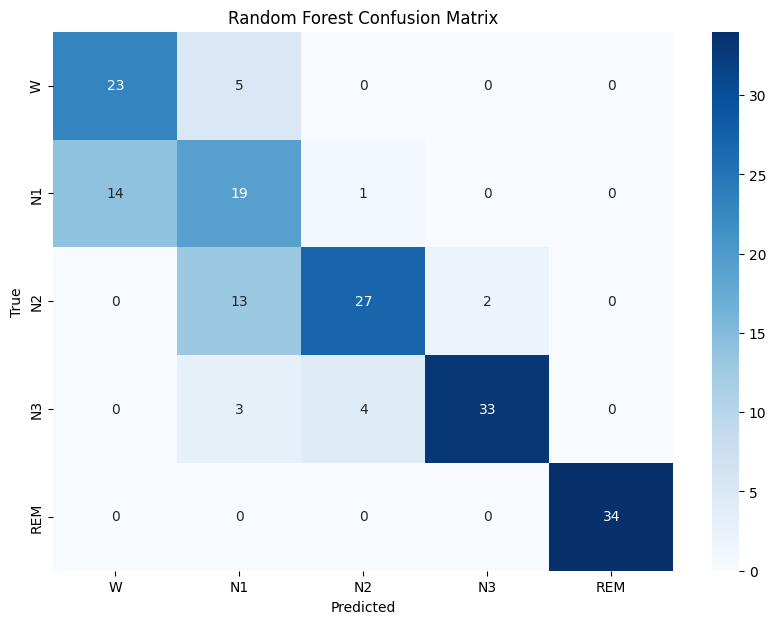
\includegraphics[width=\textwidth]{../img/paper_1/Random_forest/random_forest_confusion_matrix.png}
	\caption{Random Forest Confusion Matrix}
\end{figure}

\begin{figure}[H]
	\centering
	\includegraphics[width=\textwidth]{../img/paper_1/Random_forest/accuracy_curve.png}
	\caption{Random Forest Accuracy Curve}
\end{figure}

\begin{figure}[H]
	\centering
	\includegraphics[width=\textwidth]{../img/paper_1/Random_forest/loss_curve.png}
	\caption{Random Forest Loss Curve}
\end{figure}

\begin{figure}[H]
	\centering
	\includegraphics[width=\textwidth]{../img/paper_1/Random_forest/precision_per_class.png}
	\caption{Random Forest Precision Per Class}
\end{figure}

\subsection{Bagging Classifier}

For the Bagging Classifier model, we present the following evaluation metrics:

\begin{figure}[H]
	\centering
	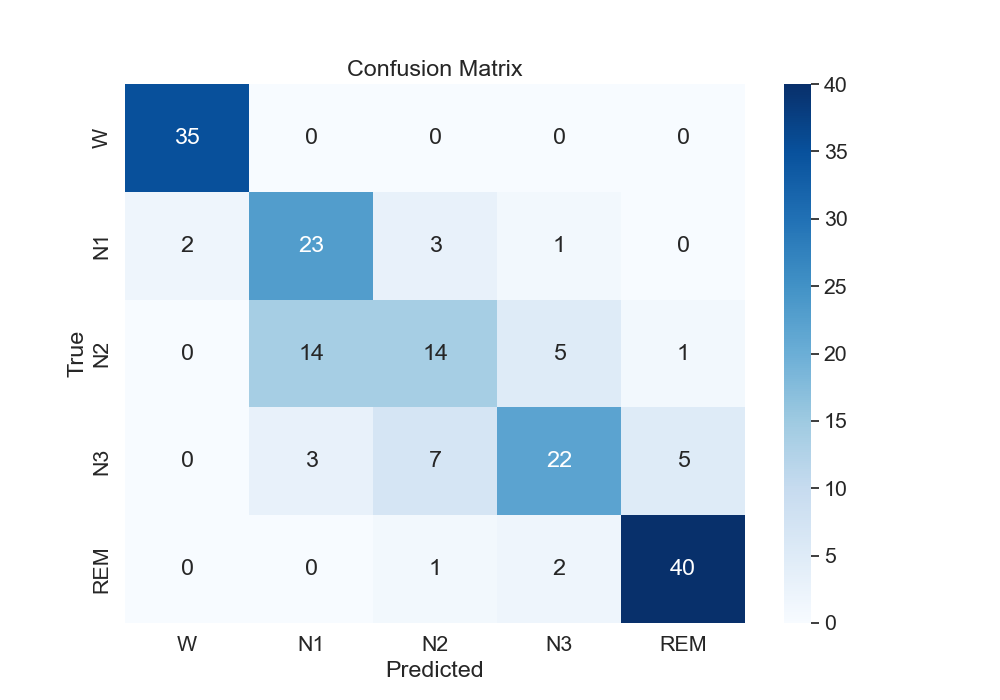
\includegraphics[width=\textwidth]{../img/paper_1/Bagging_Boosting/BG_confusion_matrix.png}
	\caption{Bagging Classifier Confusion Matrix}
\end{figure}

\begin{figure}[H]
	\centering
	\includegraphics[width=\textwidth]{../img/paper_1/Bagging_Boosting/accuracy_curve.png}
	\caption{Bagging Classifier Accuracy Curve}
\end{figure}

\begin{figure}[H]
	\centering
	\includegraphics[width=\textwidth]{../img/paper_1/Bagging_Boosting/loss_curve.png}
	\caption{Bagging Classifier Loss Curve}
\end{figure}

\begin{figure}[H]
	\centering
	\includegraphics[width=\textwidth]{../img/paper_1/Bagging_Boosting/precision_per_class.png}
	\caption{Bagging Classifier Precision Per Class}
\end{figure}

\subsection{Ensemble Learning}

For the Ensemble Learning model, we present the following evaluation metrics:

\begin{figure}[H]
	\centering
	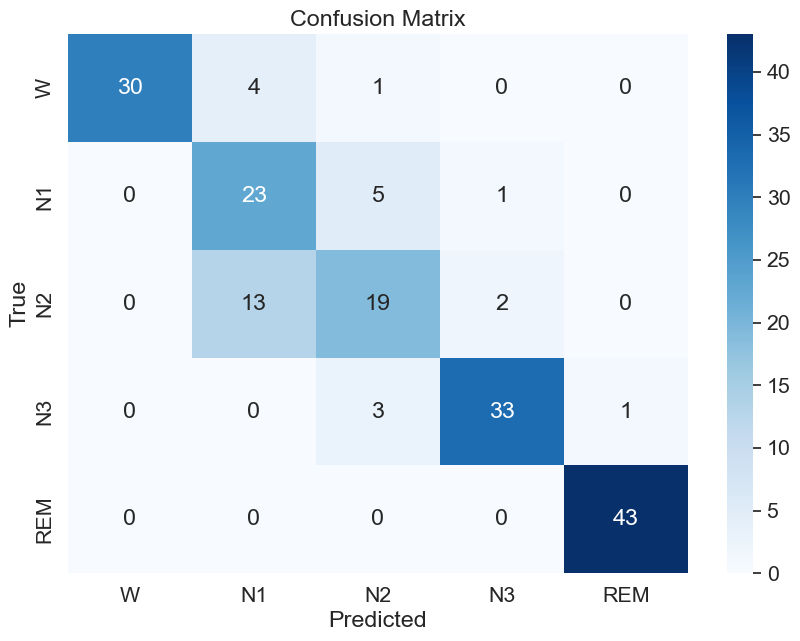
\includegraphics[width=\textwidth]{../img/paper_1/Ensemble_Learning/Ensemble_confusion_matrix.png}
	\caption{Ensemble Learning Confusion Matrix}
\end{figure}

\begin{figure}[H]
	\centering
	\includegraphics[width=\textwidth]{../img/paper_1/Ensemble_Learning/accuracy_curve.png}
	\caption{Ensemble Learning Accuracy Curve}
\end{figure}

\begin{figure}[H]
	\centering
	\includegraphics[width=\textwidth]{../img/paper_1/Ensemble_Learning/loss_curve.png}
	\caption{Ensemble Learning Loss Curve}
\end{figure}

\begin{figure}[H]
	\centering
	\includegraphics[width=\textwidth]{../img/paper_1/Ensemble_Learning/precision_per_class.png}
	\caption{Ensemble Learning Precision Per Class}
\end{figure}

\subsection{Gradient Boosting}

For the Gradient Boosting model, we present the following evaluation metrics:

\begin{figure}[H]
	\centering
	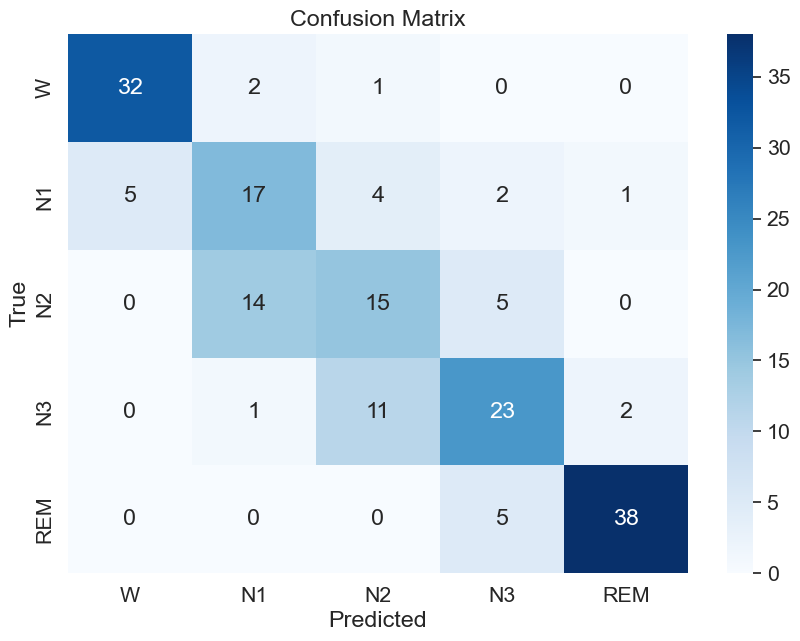
\includegraphics[width=\textwidth]{../img/paper_1/gradient_boosting/confusion_matrix.png}
	\caption{Gradient Boosting Confusion Matrix}
\end{figure}

\begin{figure}[H]
	\centering
	\includegraphics[width=\textwidth]{../img/paper_1/gradient_boosting/accuracy_curve.png}
	\caption{Gradient Boosting Accuracy Curve}
\end{figure}

\begin{figure}[H]
	\centering
	\includegraphics[width=\textwidth]{../img/paper_1/gradient_boosting/loss_curve.png}
	\caption{Gradient Boosting Loss Curve}
\end{figure}

\begin{figure}[H]
	\centering
	\includegraphics[width=\textwidth]{../img/paper_1/gradient_boosting/precision_per_class.png}
	\caption{Gradient Boosting Precision Per Class}
\end{figure}


\chapter{Deep Neural Model for Automated Sleep Staging System using Single-Channel EEG Signal}
\label{chapter_paper2}
\section{Methodology}



We employed the publicly available \textbf{Sleep-EDF} dataset for automated sleep stage classification. This dataset consists of two primary file types: Polysomnographic (PSG) recordings in European Data Format (EDF) and corresponding Hypnogram annotation files. The EDF files contain multi-channel biosignals, including EEG, while the Hypnogram files provide ground-truth sleep stage labels aligned with specific time intervals.



The dataset was partitioned into \textbf{training}, \textbf{validation}, and \textbf{testing} subsets using a \textbf{90:5:5} split. Given the inherent class imbalance in sleep stage distribution, we employed the \textbf{SMOTE} (Synthetic Minority Over-sampling Technique) to synthetically balance the dataset, improving model robustness across minority classes.


\begin{figure}[H]
	\centering
	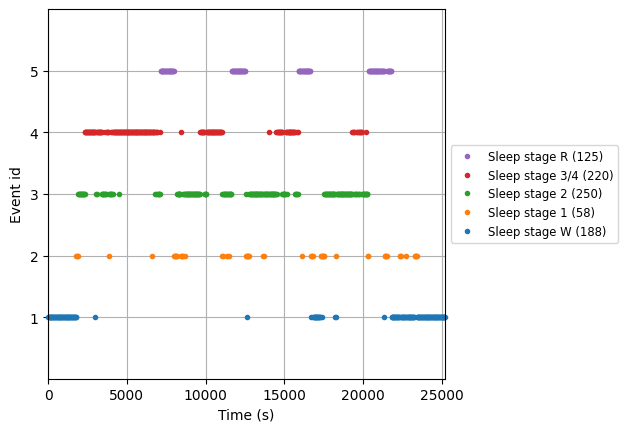
\includegraphics[width=0.60\textwidth]{img/paper_2/sleep event.PNG}
	\caption{Event Mapping Plot}
	\label{fig:lstm_accuracy}
\end{figure}


\subsection{Modeling Approach}

We implemented and evaluated several machine learning and deep learning architectures for the classification task. One of the core models used is the \textbf{Deep Neural Network (DNN)}, designed as a fully connected feedforward architecture suitable for non-sequential input.

\subsubsection{Deep Neural Network (DNN)}

The DNN consists of an input layer followed by three fully connected (\texttt{Dense}) layers comprising \textbf{128}, \textbf{64}, and \textbf{32} neurons respectively. Each layer employs the \textbf{ReLU} activation function to introduce non-linearity. To mitigate overfitting, \textbf{Dropout layers} with a dropout rate of \textbf{0.2} were interleaved between each dense layer. The final output layer uses a \textbf{Softmax} activation to produce class probabilities for the five sleep stages.




\section{Dataset Information}


ensure efficient implementation and reproducibility, this research adheres to a well-structured computational framework, including consistent system configuration, version control, and the integration of essential libraries for data processing and deep learning tasks. The experiments were conducted on both Windows and Linux operating systems using an \textbf{Intel Core i5 11th Gen} processor (with \textit{Iris Xe Graphics} and a clock speed of \textbf{3.9 GHz}). The programming environment was built with \textbf{Python version 3.13.1}, managed via the \texttt{pip} package installer.

The study utilized the \textbf{Sleep-EDF} dataset, which contains EEG recordings and corresponding hypnograms for sleep stage classification. Prior to model training, the dataset was preprocessed into uniform, fixed-length segments. The dataset is publicly available at: \url{https://www.physionet.org/content/sleep-edf/1.0.0/}.

For project collaboration and version control, \textbf{GitHub} was employed, with the full implementation accessible at: \url{https://github.com/tanmay007thor/ContraWR}.

Several key libraries were used throughout the development pipeline:
\begin{itemize}
	\item \textbf{NumPy (2.2.2)} – Numerical computations
	\item \textbf{scikit-learn (1.6.1)} – Machine learning utilities
	\item \textbf{imbalanced-learn (0.13.0)} – Handling class imbalance (SMOTE)
	\item \textbf{MNE (1.9.0)} – EEG signal processing
	\item \textbf{TensorFlow/Keras (2.16.1)} – Deep learning model implementation
	\item \textbf{Matplotlib (3.10.0)} and \textbf{Seaborn (0.13.2)} – Data visualization
\end{itemize}

This setup ensures smooth execution of machine learning and deep learning models, including BiLSTM and other architectures, for automating sleep stage classification.



\section{Preprocessing Techniques}

To ensure consistency in the input data, all recordings were resampled to a \textbf{100 Hz} sampling frequency. Each signal was segmented into \textbf{30-second epochs}, resulting in \textbf{3000 time steps per sample}. These samples were stored in \texttt{PKL} (Pickle) format, each approximately \textbf{48 KB} in size, enabling efficient storage and fast access, particularly beneficial for edge device deployment.

Each sample consisted of input-output pairs: the inputs ($X$) included two EEG channels—\textbf{FPZ-CZ} and \textbf{PZ-OZ}—while the labels ($Y$) represented the corresponding sleep stages. The stages were categorized into five classes: \textbf{Wake, N1, N2, N3,} and \textbf{REM}. To streamline processing, raw labels were mapped to a standardized class format.




\section{Model Architecture and Learning Framework}


\subsubsection{Deep Neural Network (DNN)}

A Deep Neural Network (DNN) is a type of multilayer feedforward architecture composed of successive fully connected layers. In this model, the input layer is followed by three dense layers containing 128, 64, and 32 neurons respectively. Each dense layer uses the Rectified Linear Unit (ReLU) activation function to introduce non-linearity.

To improve generalization and prevent overfitting, dropout layers with a dropout rate of 0.2 are inserted between the dense layers. The final output layer employs a Softmax activation function to map the learned features to the five target sleep stages: Wake, N1, N2, N3, and REM.

\begin{table}[H]
	\centering
	\caption{Architecture of the Deep Neural Network}
	\label{tab:nn_architecture}
	\begin{tabular}{lcc}
		\hline
		\textbf{Layer Type} & \textbf{Units} & \textbf{Activation Function} \\
		\hline
		Input Layer         & \texttt{X\_train}          & - \\
		Dense Layer         & 128                        & ReLU \\
		Dropout Layer       & -                          & 0.2 (Dropout Rate) \\
		Dense Layer         & 64                         & ReLU \\
		Dropout Layer       & -                          & 0.2 (Dropout Rate) \\
		Dense Layer         & 32                         & ReLU \\
		Dropout Layer       & -                          & 0.2 (Dropout Rate) \\
		Output Layer        & Number of classes (e.g., 5) & Softmax \\
		\hline
	\end{tabular}
\end{table}

While DNNs are effective in extracting complex feature representations from EEG signals, they are inherently limited in modeling temporal dependencies due to their feedforward nature. This limits their standalone utility for time-series classification tasks like sleep staging.

\subsubsection{Forward Propagation}

Forward propagation computes the activations at each layer using the following equations:

\begin{align}
	z^{(l)} &= W^{(l)} a^{(l-1)} + b^{(l)} \\
	a^{(l)} &= \sigma(z^{(l)})
\end{align}

\noindent where:
\begin{itemize}
	\item \( z^{(l)} \) is the pre-activation (linear combination of inputs) at layer \( l \),
	\item \( a^{(l)} \) is the activation output at layer \( l \),
	\item \( W^{(l)} \) and \( b^{(l)} \) denote the weights and biases of layer \( l \),
	\item \( \sigma \) is the activation function (ReLU or Softmax depending on the layer).
\end{itemize}

\subsubsection{Backward Propagation}

During training, gradients of the loss function with respect to weights and biases are calculated using backpropagation. The process involves the following steps:

\begin{align}
	\delta^{(L)} &= \frac{\partial L}{\partial a^{(L)}} \odot \sigma'(z^{(L)}) \\
	\delta^{(l)} &= \left(W^{(l+1)}\right)^T \delta^{(l+1)} \odot \sigma'(z^{(l)}) \\
	\frac{\partial L}{\partial W^{(l)}} &= \delta^{(l)} \left(a^{(l-1)}\right)^T \\
	\frac{\partial L}{\partial b^{(l)}} &= \sum \delta^{(l)}
\end{align}

\noindent where:
\begin{itemize}
	\item \( \delta^{(l)} \) is the error signal at layer \( l \),
	\item \( \sigma'(z^{(l)}) \) is the derivative of the activation function,
	\item \( \frac{\partial L}{\partial W^{(l)}} \) and \( \frac{\partial L}{\partial b^{(l)}} \) are gradients used for weight and bias updates.
\end{itemize}

\subsubsection{Activation Functions}

The Softmax function is used in the output layer to produce class probabilities:

\begin{equation}
	\sigma(z_i) = \frac{e^{z_i}}{\sum_{j=1}^{N} e^{z_j}}
\end{equation}

\noindent where:
\begin{itemize}
	\item \( z_i \) is the input to the \( i^{th} \) output neuron,
	\item \( N \) is the number of output classes,
	\item The denominator ensures the outputs form a probability distribution summing to 1.
\end{itemize}

For hidden layers, the ReLU activation function is applied:

\begin{equation}
	f(x) = \max(0, x)
\end{equation}

\noindent where:
\begin{itemize}
	\item \( x \) is the input to the neuron,
	\item The function outputs \( x \) if \( x > 0 \), and 0 otherwise.
\end{itemize}


\subsubsection{Recurrent Neural Network (RNN)}

Recurrent Neural Networks (RNNs) are specifically designed for modeling sequential data by incorporating feedback connections, allowing them to retain information across time steps. This architecture is well-suited for EEG signal analysis due to its ability to capture temporal dependencies.

In the proposed model, two RNN layers are employed: the first with 128 units and the second with 64 units, both using the Tanh activation function. These layers process sequential inputs while maintaining internal memory of past computations.

\begin{table}[!h]
	\centering
	\caption{Recurrent Neural Network Architecture for Sleep Stage Classification}
	\label{tab:rnn_architecture}
	\begin{tabular}{lcc}
		\hline
		\textbf{Layer Type} & \textbf{Units} & \textbf{Activation Function} \\
		\hline
		Input Layer         & \texttt{X\_train}          & - \\
		RNN Layer 1         & 128                        & Tanh \\
		Dropout Layer       & -                          & 0.2 (Dropout Rate) \\
		RNN Layer 2         & 64                         & Tanh \\
		Dropout Layer       & -                          & 0.2 (Dropout Rate) \\
		Dense Layer         & 64                         & ReLU \\
		Dropout Layer       & -                          & 0.2 (Dropout Rate) \\
		Dense Layer         & 32                         & ReLU \\
		Dropout Layer       & -                          & 0.2 (Dropout Rate) \\
		Output Layer        & Number of classes (e.g., 5) & Softmax \\
		\hline
	\end{tabular}
\end{table}

Dropout layers with a 0.2 rate are introduced after each RNN and dense layer to mitigate overfitting. The dense layers, activated using ReLU, help to refine temporal features extracted by the RNN layers. The final classification is performed by a Softmax-activated output layer corresponding to the target sleep stages.

Although RNNs are effective for learning short-term dependencies in sequential EEG data, they are prone to issues such as vanishing gradients, which can hinder the learning of long-range patterns.

The operation of an RNN cell at each time step \( t \) is mathematically represented as:

\begin{equation}
	h_t = \tanh(W_h h_{t-1} + W_x x_t + b_h)
\end{equation}

\noindent where:
\begin{itemize}
	\item \( h_t \) is the hidden state at time step \( t \),
	\item \( x_t \) is the input at time step \( t \),
	\item \( W_h \) and \( W_x \) are the recurrent and input weight matrices, respectively,
	\item \( b_h \) is the bias vector,
	\item \( \tanh \) is the hyperbolic tangent activation function.
\end{itemize}



\subsubsection{Long Short-Term Memory (LSTM)}

Long Short-Term Memory (LSTM) networks extend traditional RNNs by incorporating memory cells and gating mechanisms, enabling them to retain long-term dependencies in sequential data. This makes them particularly effective for time-series applications like EEG-based sleep stage classification.

The proposed LSTM architecture includes two stacked LSTM layers with 128 and 64 units, respectively, both using the Tanh activation function to handle nonlinear temporal patterns in the data. To prevent overfitting, dropout layers with a rate of 0.2 are placed after each LSTM and dense layer.

\begin{table}[H]
	\centering
	\caption{LSTM Neural Network Architecture for Sleep Stage Classification}
	\label{tab:lstm_architecture}
	\begin{tabular}{lcc}
		\hline
		\textbf{Layer Type} & \textbf{Units} & \textbf{Activation Function} \\
		\hline
		Input Layer         & \texttt{X\_train}           & - \\
		LSTM Layer 1        & 128                         & Tanh \\
		Dropout Layer       & -                           & 0.2 (Dropout Rate) \\
		LSTM Layer 2        & 64                          & Tanh \\
		Dropout Layer       & -                           & 0.2 (Dropout Rate) \\
		Dense Layer         & 64                          & ReLU \\
		Dropout Layer       & -                           & 0.2 (Dropout Rate) \\
		Dense Layer         & 32                          & ReLU \\
		Dropout Layer       & -                           & 0.2 (Dropout Rate) \\
		Output Layer        & Number of classes (e.g., 5) & Softmax \\
		\hline
	\end{tabular}
\end{table}

The dense layers following the LSTM blocks (with 64 and 32 units) refine the extracted temporal features using ReLU activations. The final output layer uses the Softmax function to perform multi-class classification of sleep stages. LSTM models are particularly advantageous in capturing long-range dependencies and complex temporal dynamics, thus often outperforming simple RNNs for EEG sequence modeling.

LSTM cells operate through a series of gating mechanisms that regulate the flow of information. The key equations governing an LSTM cell at time step \( t \) are:

\begin{align}
	f_t &= \sigma(W_f x_t + U_f h_{t-1} + b_f) \quad \text{(Forget Gate)} \\
	i_t &= \sigma(W_i x_t + U_i h_{t-1} + b_i) \quad \text{(Input Gate)} \\
	\tilde{c}t &= \tanh(W_c x_t + U_c h{t-1} + b_c) \quad \text{(Candidate Cell State)} \\
	c_t &= f_t \odot c_{t-1} + i_t \odot \tilde{c}_t \quad \text{(Cell State Update)} \\
	o_t &= \sigma(W_o x_t + U_o h_{t-1} + b_o) \quad \text{(Output Gate)} \\
	h_t &= o_t \odot \tanh(c_t) \quad \text{(Hidden State Update)}
\end{align}

\noindent where:
\begin{itemize}
	\item \( f_t, i_t, o_t \) represent the forget, input, and output gates, respectively.
	\item \( \tilde{c}_t \) is the candidate cell state.
	\item \( c_t \) is the updated memory cell state.
	\item \( h_t \) is the hidden state at time \( t \).
	\item \( \sigma \) denotes the sigmoid activation function.
	\item \( \odot \) represents element-wise multiplication.
	\item \( W, U, b \) are the learned weight matrices and biases.
\end{itemize}


\subsubsection{Bidirectional Long Short-Term Memory (Bi-LSTM)}

The Bidirectional Long Short-Term Memory (Bi-LSTM) network enhances the LSTM model by processing input sequences in both forward and backward directions, enabling the model to learn context from both past and future data. This bidirectional approach improves the model's ability to capture dependencies in temporal data, making it highly effective for tasks such as EEG-based sleep stage classification.

The architecture consists of two bidirectional LSTM layers with 128 and 64 units, respectively, both utilizing the Tanh activation function. Dropout layers (with a rate of 0.2) are applied after each LSTM layer to prevent overfitting. Following the bidirectional LSTM layers, dense layers with 64 and 32 units, using ReLU activation, are added to refine the learned features before the final classification layer, which uses the Softmax activation to classify the sleep stages.

\begin{table}[!h]
	\centering
	\caption{Bidirectional LSTM Neural Network Architecture for Sleep Stage Classification}
	\label{tab:bi_lstm_architecture}
	\begin{tabular}{lcc}
		\hline
		\textbf{Layer Type} & \textbf{Units} & \textbf{Activation Function} \\
		\hline
		Input Layer         & \texttt{X\_train}            & - \\
		Bi-LSTM Layer 1     & 128                          & Tanh \\
		Dropout Layer       & -                            & 0.2 (Dropout Rate) \\
		Bi-LSTM Layer 2     & 64                           & Tanh \\
		Dropout Layer       & -                            & 0.2 (Dropout Rate) \\
		Dense Layer         & 64                           & ReLU \\
		Dropout Layer       & -                            & 0.2 (Dropout Rate) \\
		Dense Layer         & 32                           & ReLU \\
		Dropout Layer       & -                            & 0.2 (Dropout Rate) \\
		Output Layer        & Number of classes (e.g., 5)  & Softmax \\
		\hline
	\end{tabular}
\end{table}

Bi-LSTM networks are particularly well-suited for EEG-based sleep stage classification, as they allow the model to capture both past and future dependencies in the EEG signal, leading to improved accuracy in detecting sleep patterns.

The Bi-LSTM model processes input sequences in both forward and backward directions, maintaining two hidden states for each timestep. The key equations describing the forward and backward passes are:

\begin{align}
	\overrightarrow{h}t &= \text{LSTM}(x_t, \overrightarrow{h}{t-1}) \\
	\overleftarrow{h}t &= \text{LSTM}(x_t, \overleftarrow{h}{t+1}) \\
	h_t &= [\overrightarrow{h}_t; \overleftarrow{h}_t]
\end{align}

where:
\begin{itemize}
	\item \( \overrightarrow{h}_t \) is the forward LSTM hidden state at time step \( t \).
	\item \( \overleftarrow{h}_t \) is the backward LSTM hidden state at time step \( t \).
	\item \( h_t \) is the concatenated hidden state, combining both forward and backward states, used for final predictions.
\end{itemize}








\section{Results and Evaluation}





\subsection{Neural Network (NN) Model}

\begin{figure}[H]
	\centering
	\begin{minipage}{0.66\textwidth}
		\centering
		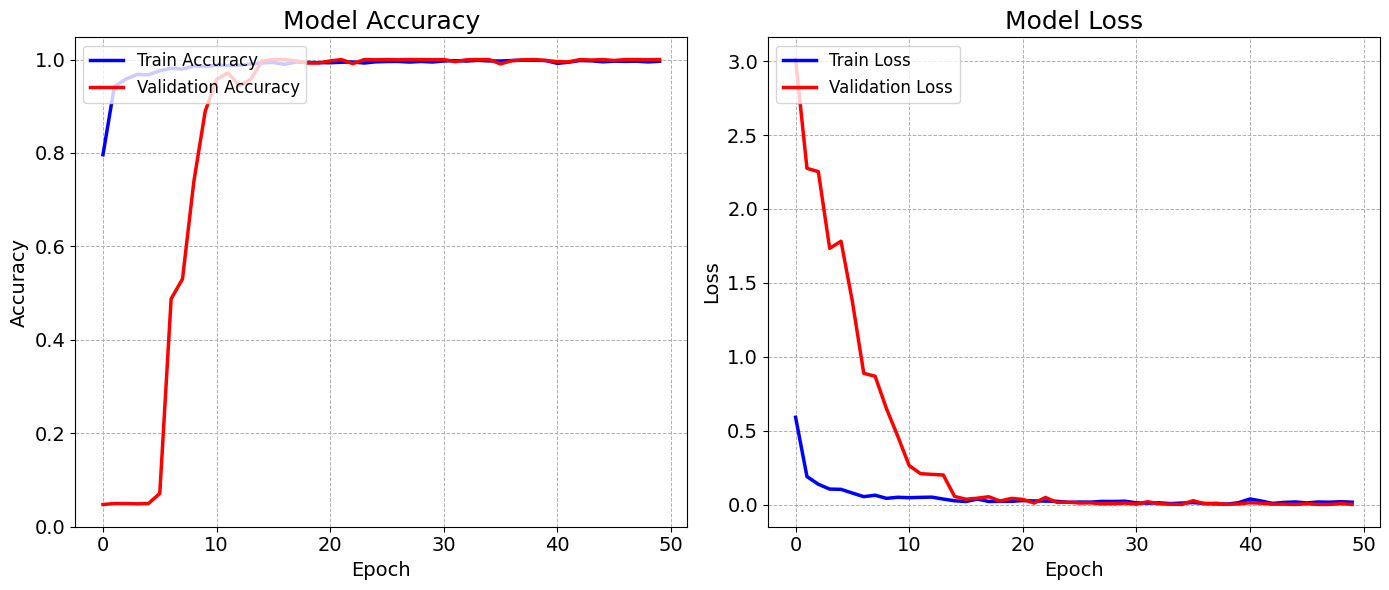
\includegraphics[width=\linewidth]{img/paper_2/deeplearning.png}
		\caption{Neural Network Accuracy and Loss Comparison}
		\label{fig:nn_accuracy}
	\end{minipage}
	\hfill
	\begin{minipage}{0.33\textwidth}
		\centering
		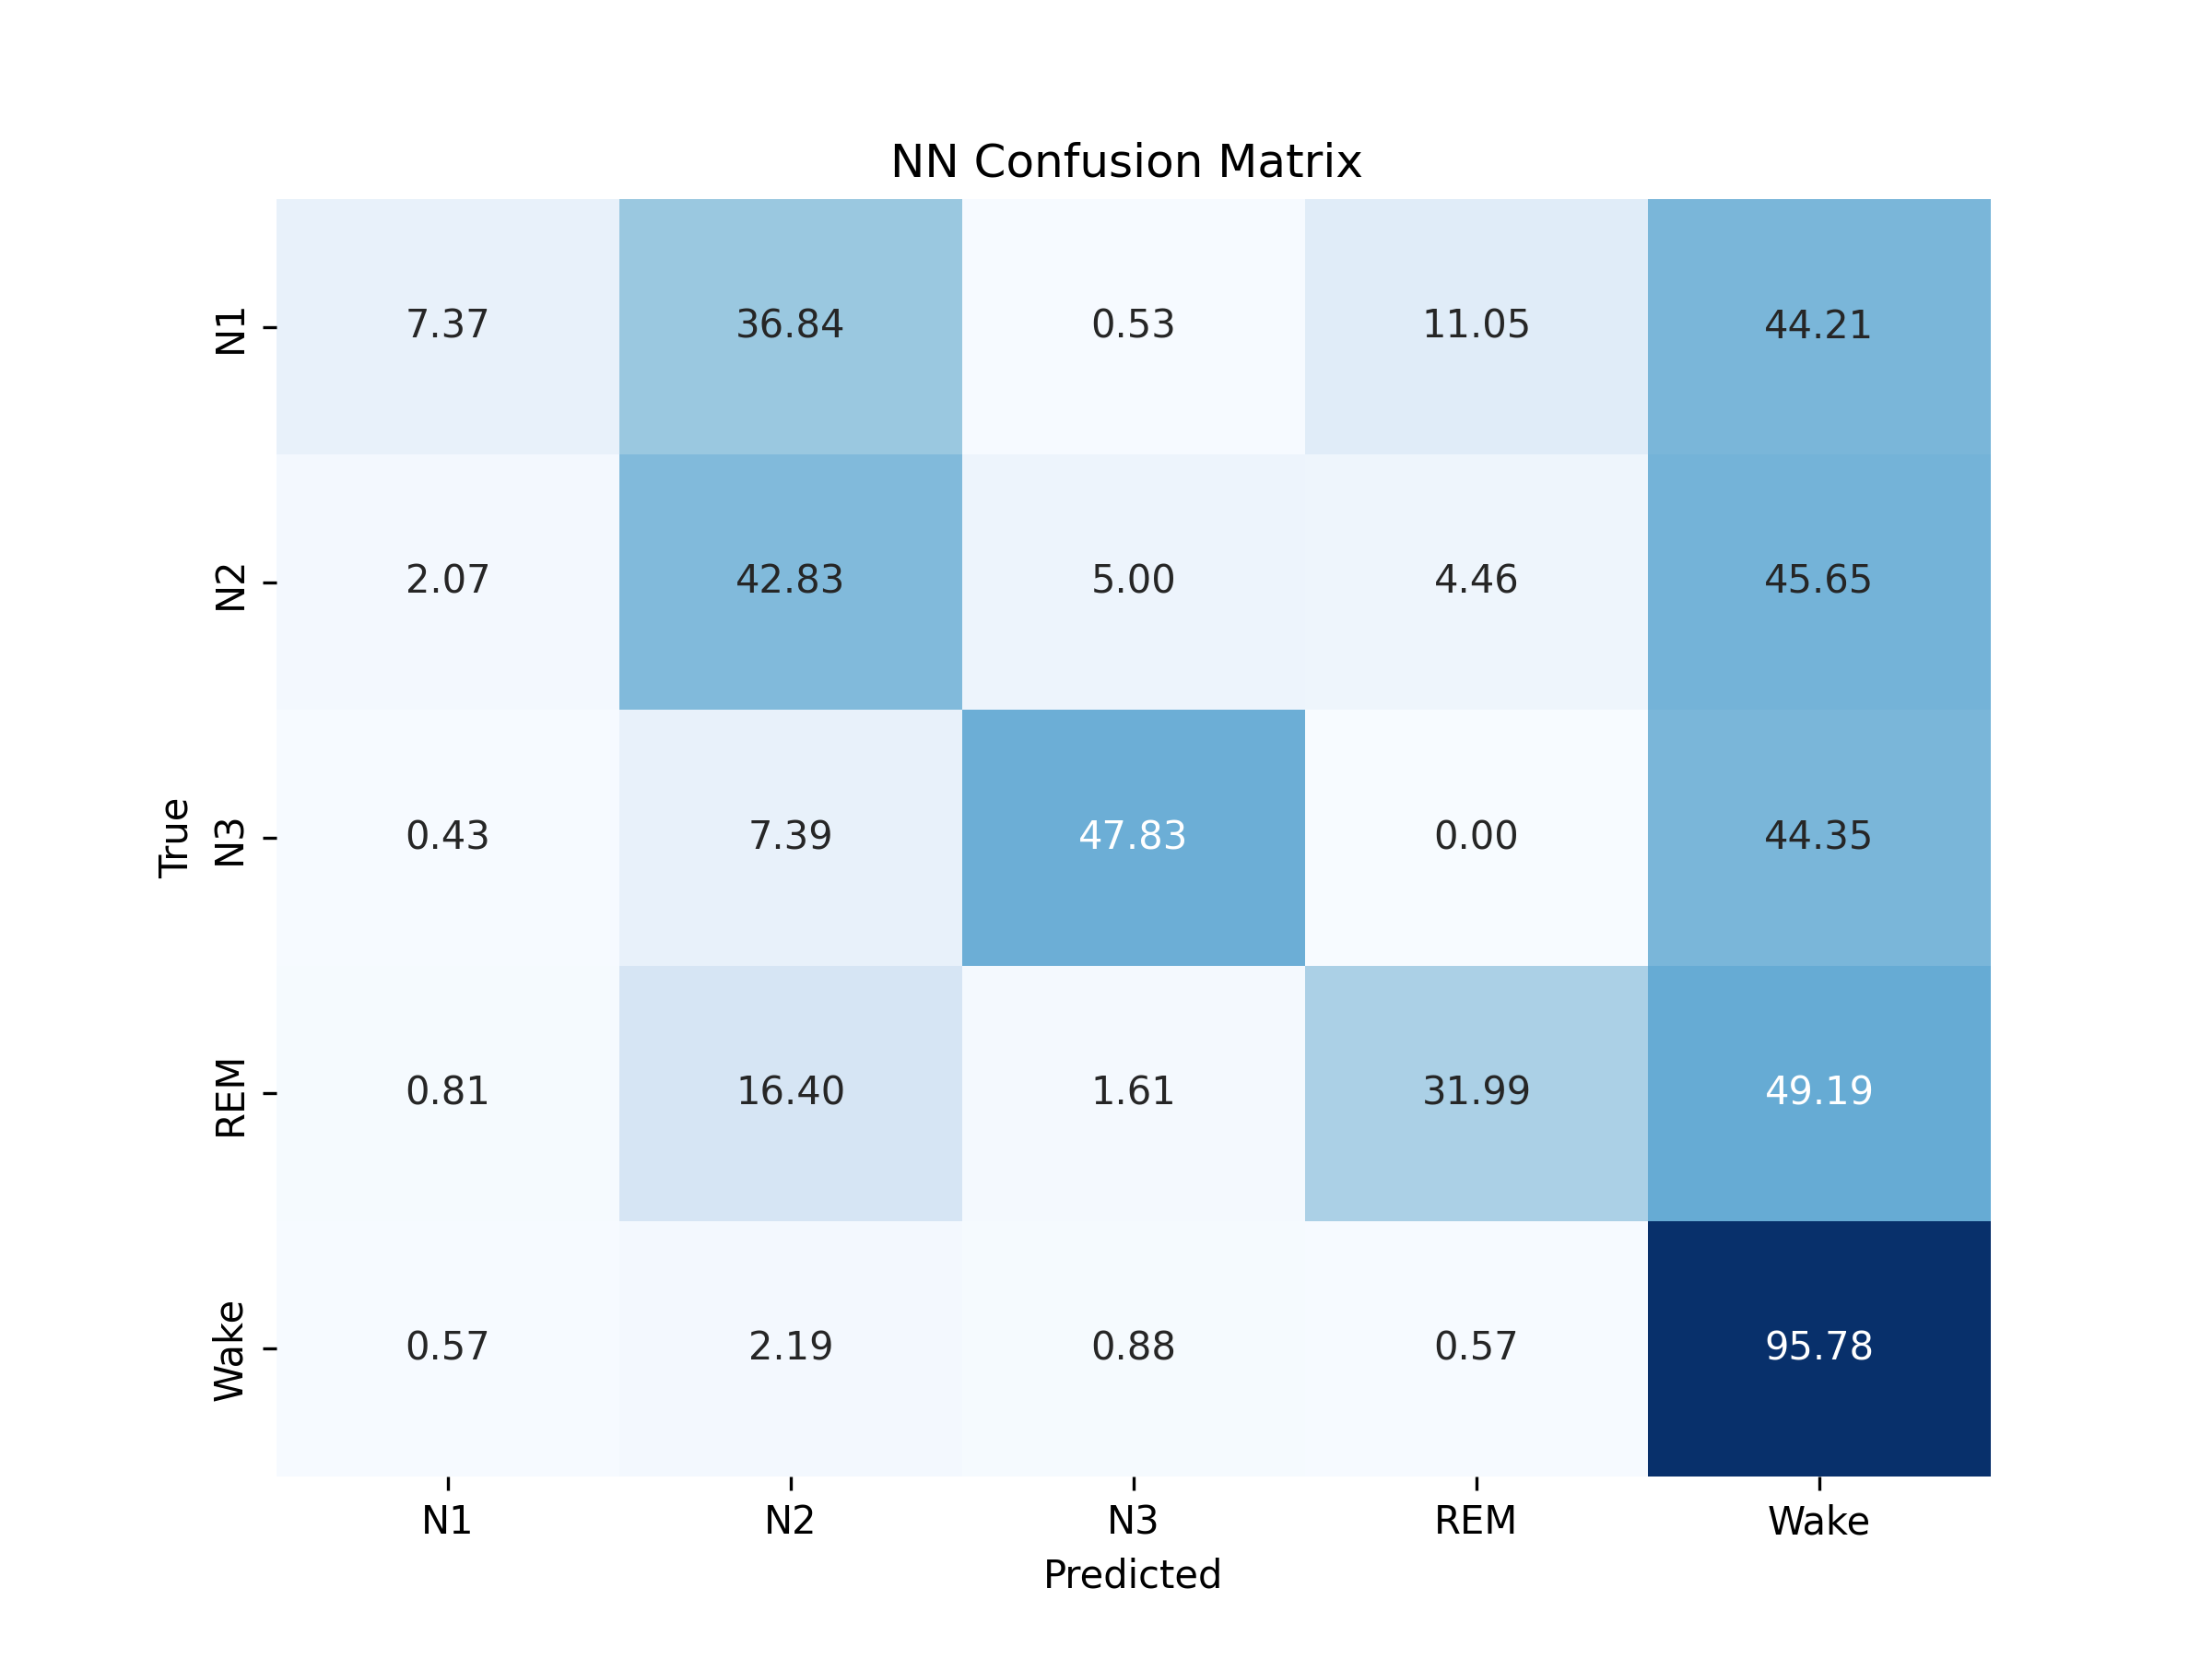
\includegraphics[width=\linewidth]{img/paper_2/NN_cm.png}
		\caption{Neural Network Confusion Matrix}
		\label{fig:nn_cm}
	\end{minipage}
\end{figure}


\subsection{LSTM Model}

\begin{figure}[H]
	\centering
	\begin{minipage}{0.66\textwidth}
		\centering
		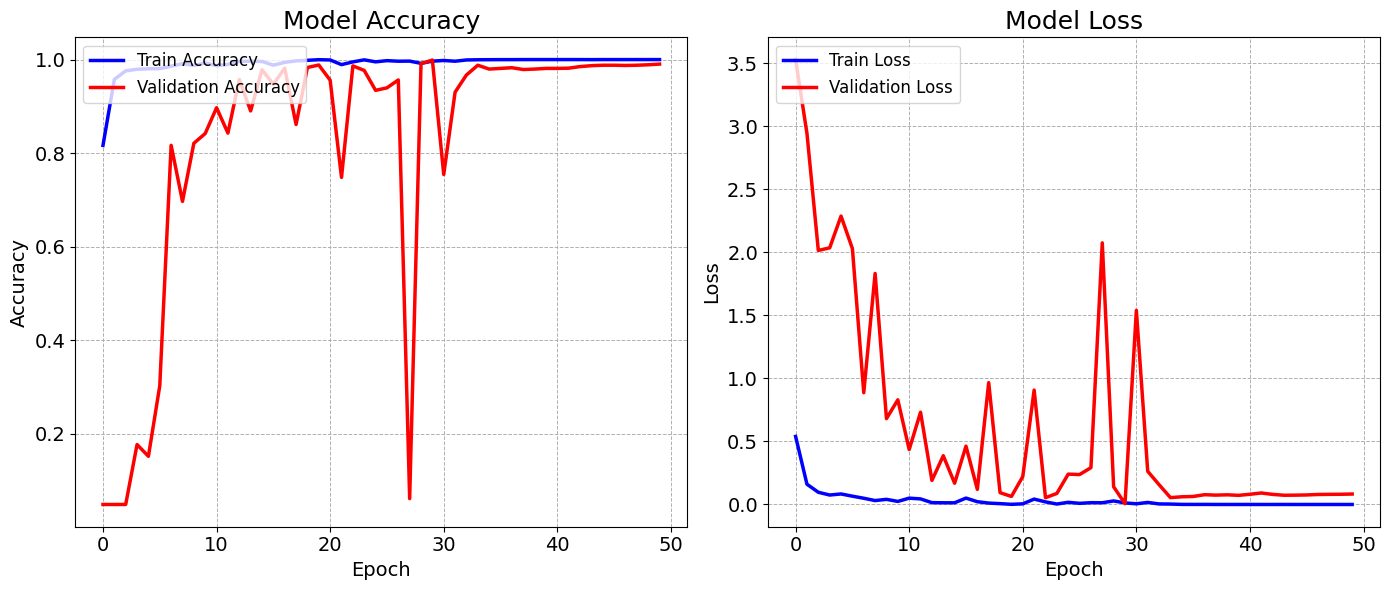
\includegraphics[width=\linewidth]{img/paper_2/lstm accuracy and loss plot.png}
		\caption{LSTM Accuracy and Loss Plot}
		\label{fig:lstm_accuracy}
	\end{minipage}
	\hfill
	\begin{minipage}{0.32\textwidth}
		\centering
		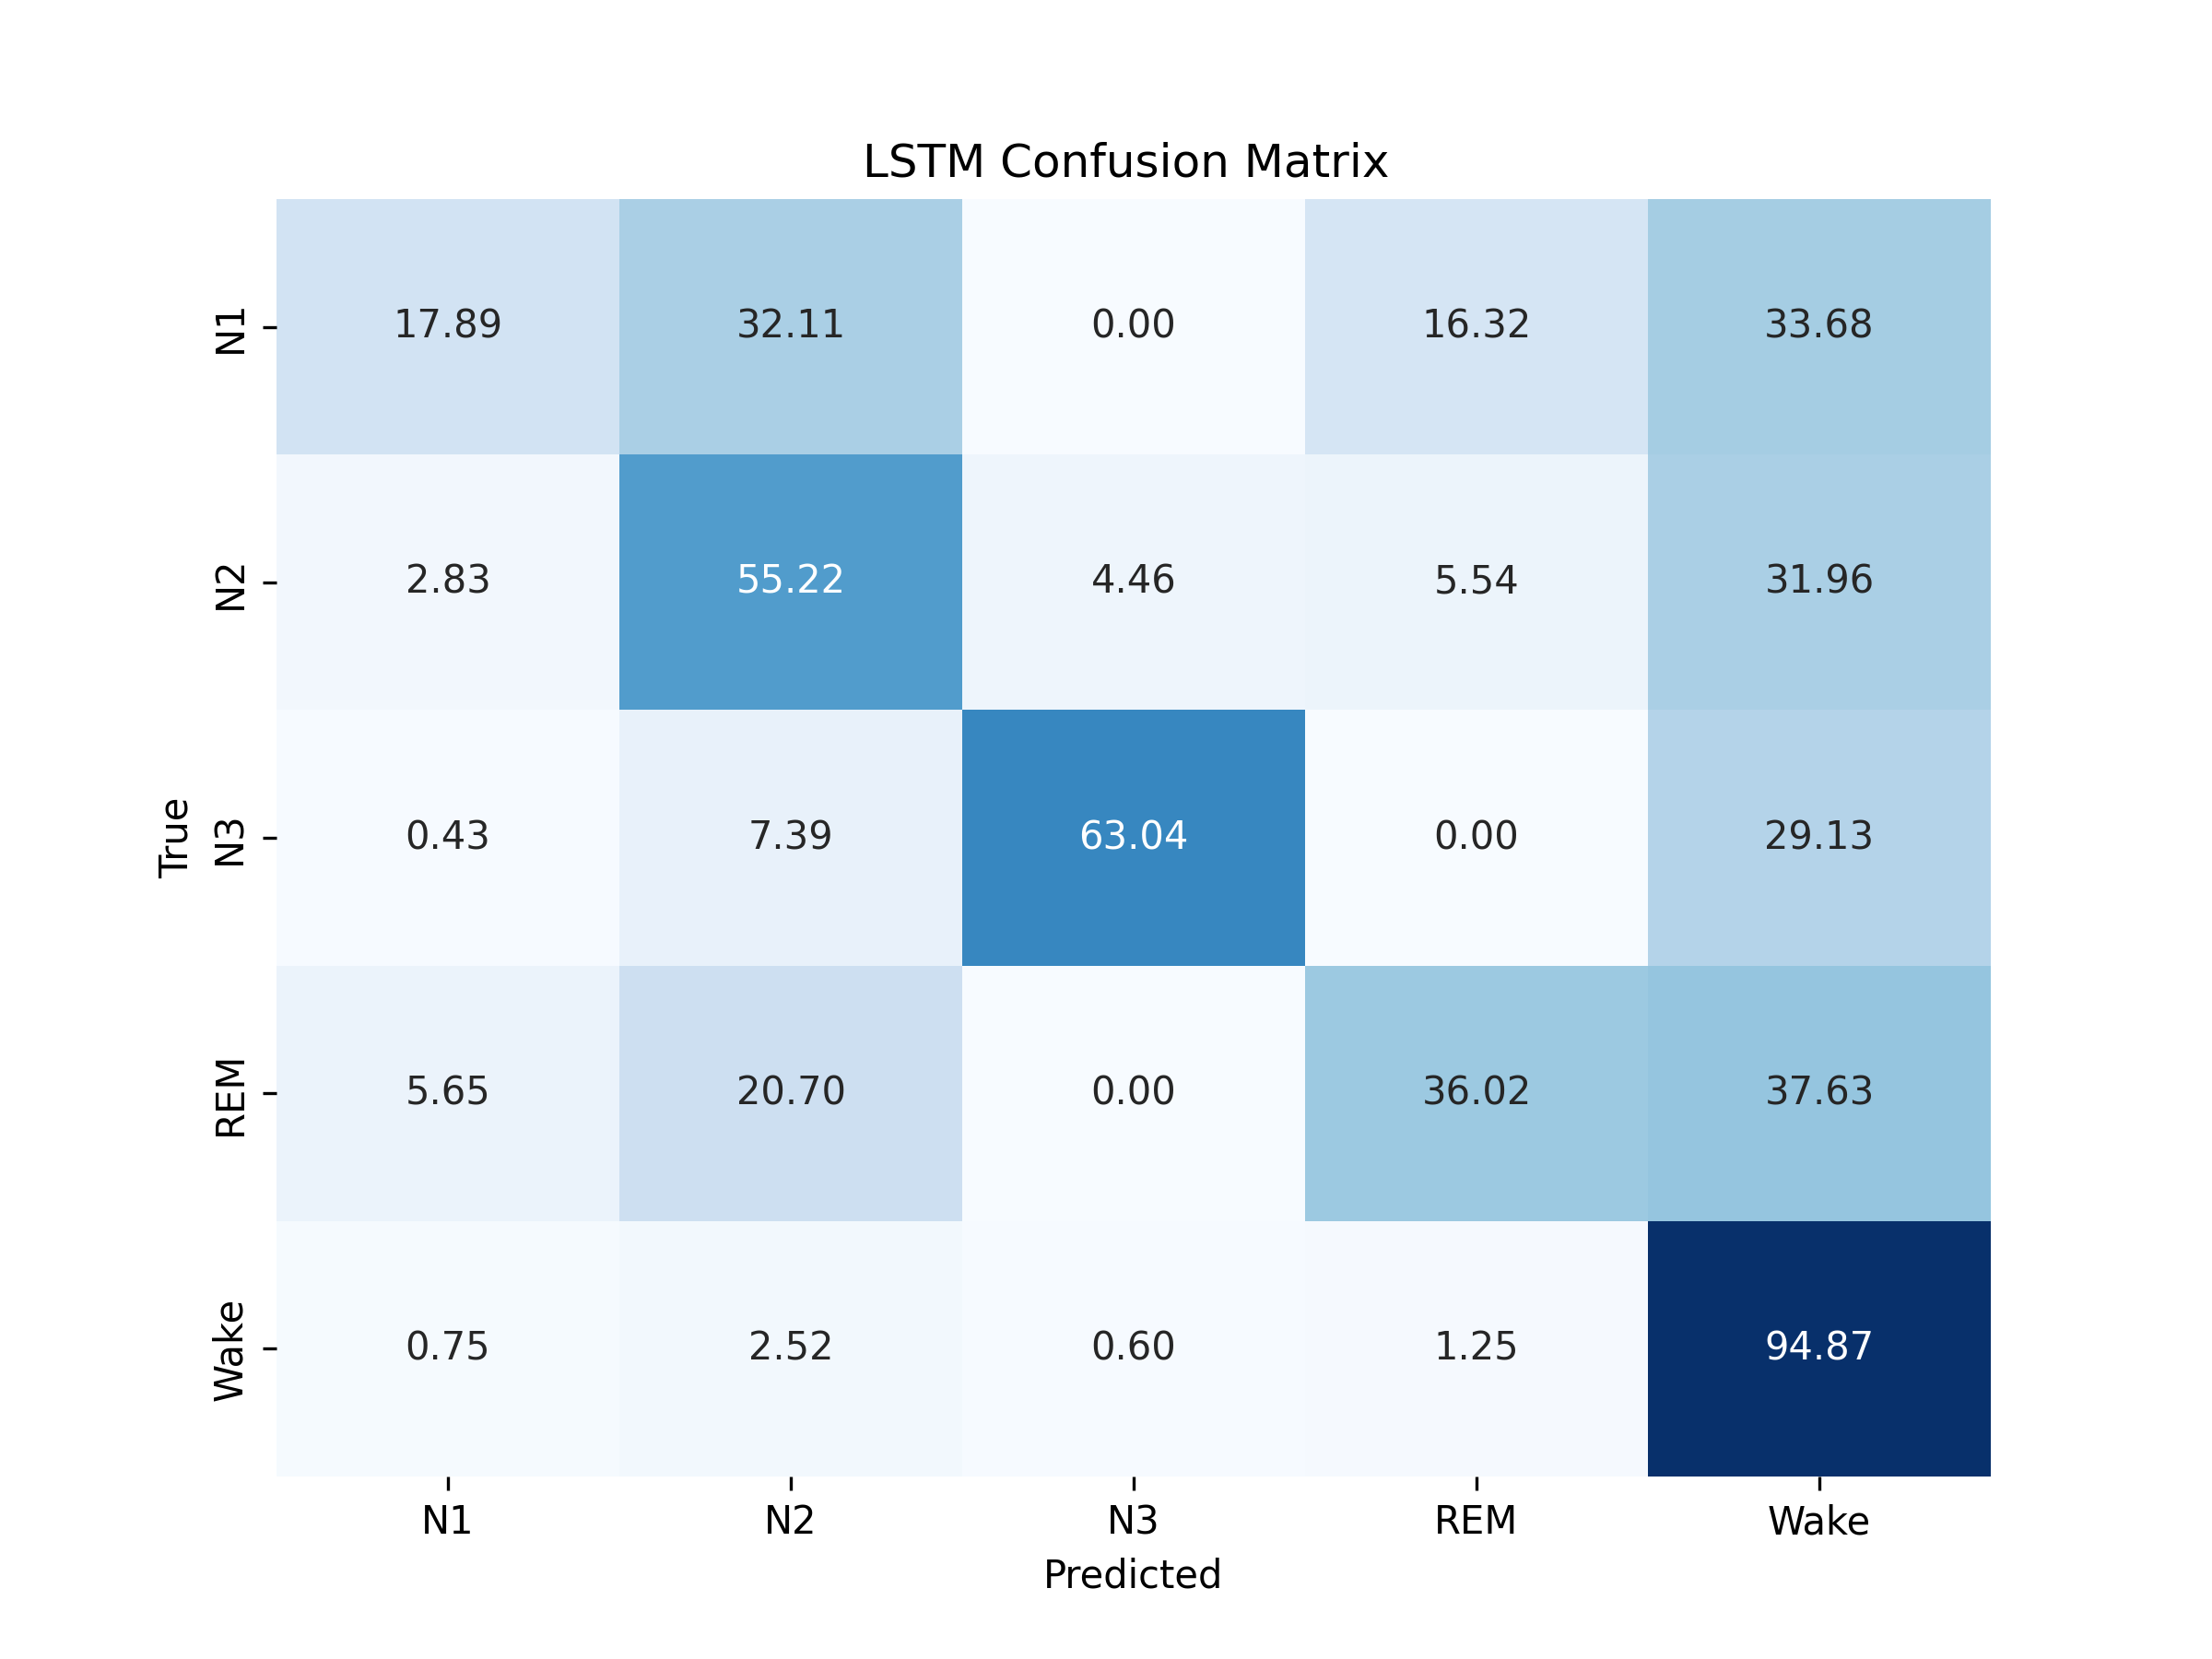
\includegraphics[width=\linewidth]{img/paper_2/LSTM_cm.png}
		\caption{LSTM Confusion Matrix}
		\label{fig:lstm_cm}
	\end{minipage}
\end{figure}


\subsection{RNN Model}

\begin{figure}[H]
	\centering
	\begin{minipage}{0.66\textwidth}
		\centering
		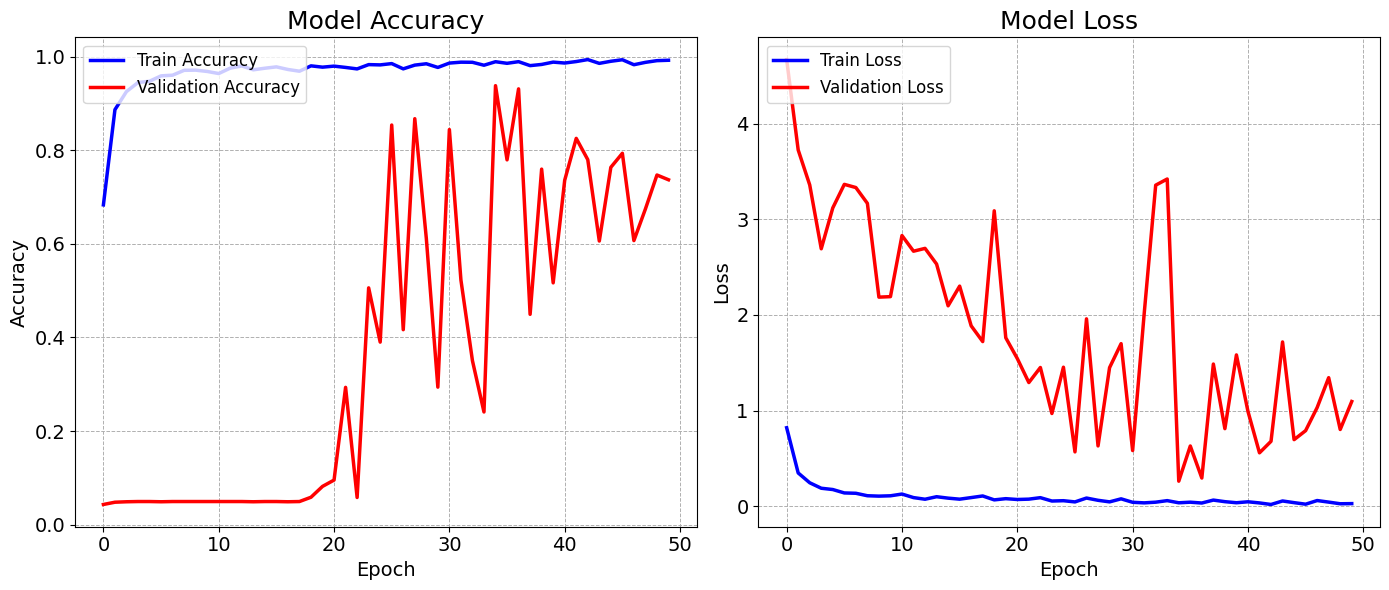
\includegraphics[width=\linewidth]{img/paper_2/Rnn Accuracy Plot.png}
		\caption{RNN Accuracy Plot}
		\label{fig:rnn_accuracy}
	\end{minipage}
	\hfill
	\begin{minipage}{0.32\textwidth}
		\centering
		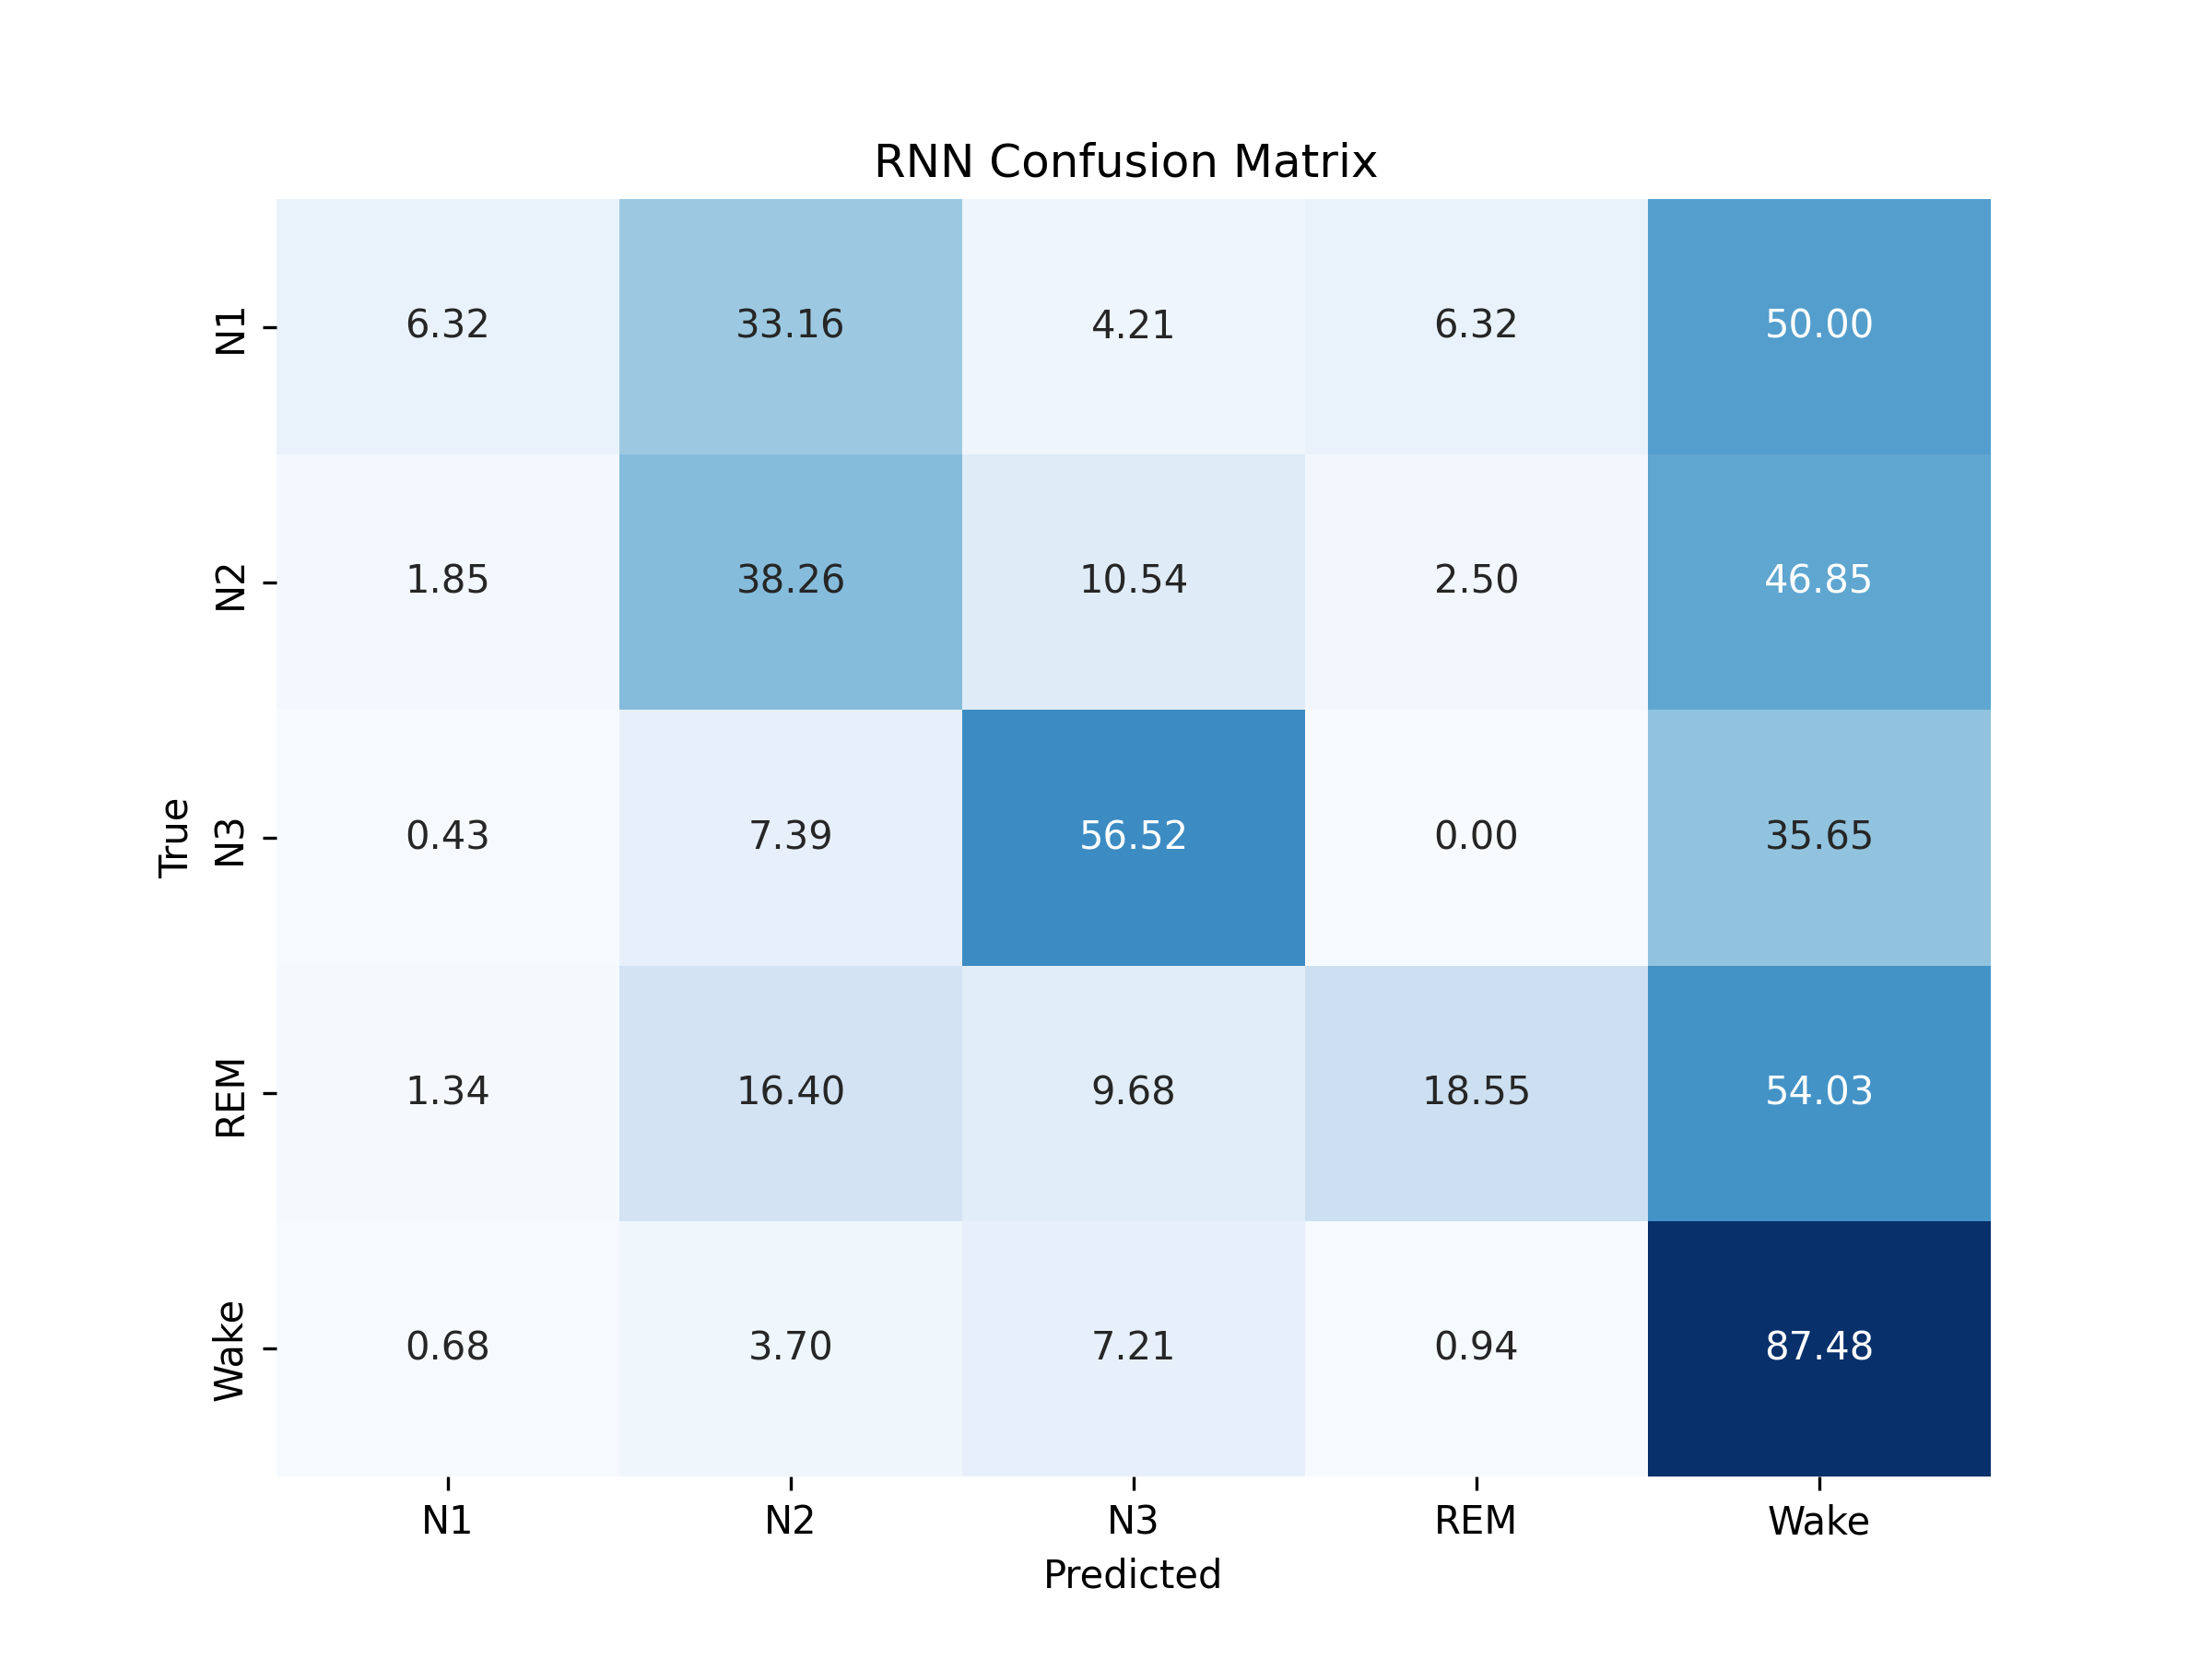
\includegraphics[width=\linewidth]{img/paper_2/RNN_cm.png}
		\caption{RNN Confusion Matrix}
		\label{fig:rnn_cm}
	\end{minipage}
\end{figure}


\subsection{BiLSTM Model}

\begin{figure}[H]
	\centering
	\begin{minipage}{0.66\textwidth}
		\centering
		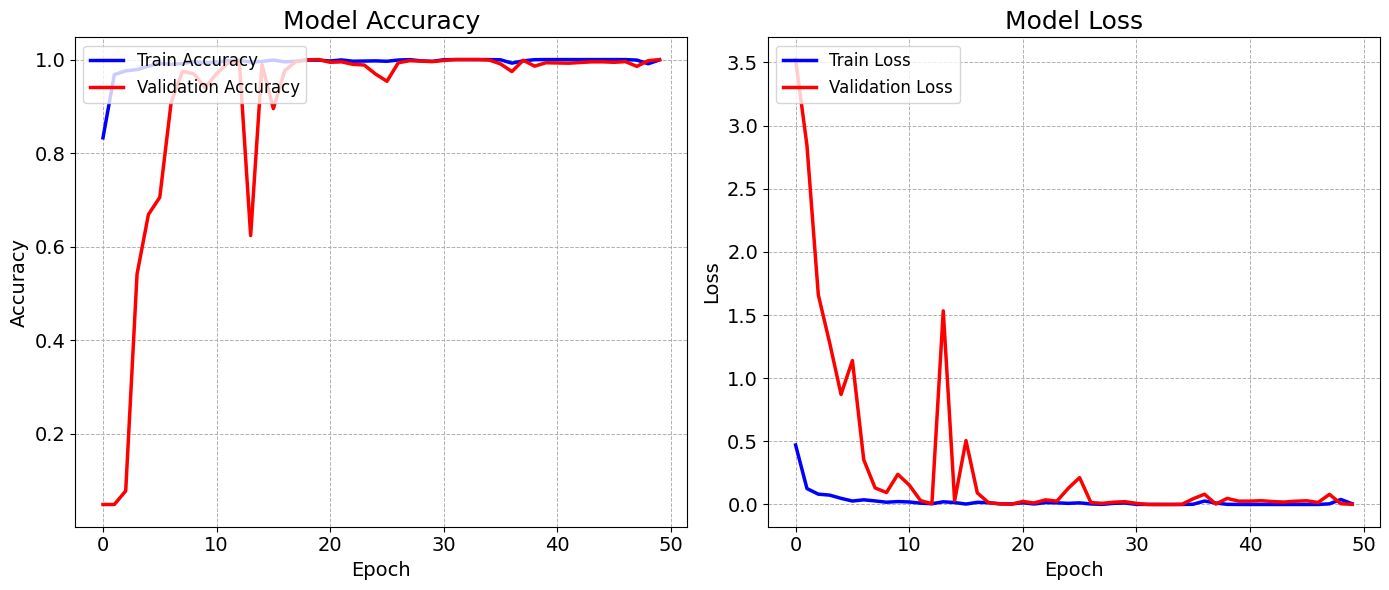
\includegraphics[width=\linewidth]{img/paper_2/BILSTM Accuaracy Plot.png}
		\caption{BiLSTM Accuracy Plot}
		\label{fig:bilstm_accuracy}
	\end{minipage}
	\hfill
	\begin{minipage}{0.32\textwidth}
		\centering
		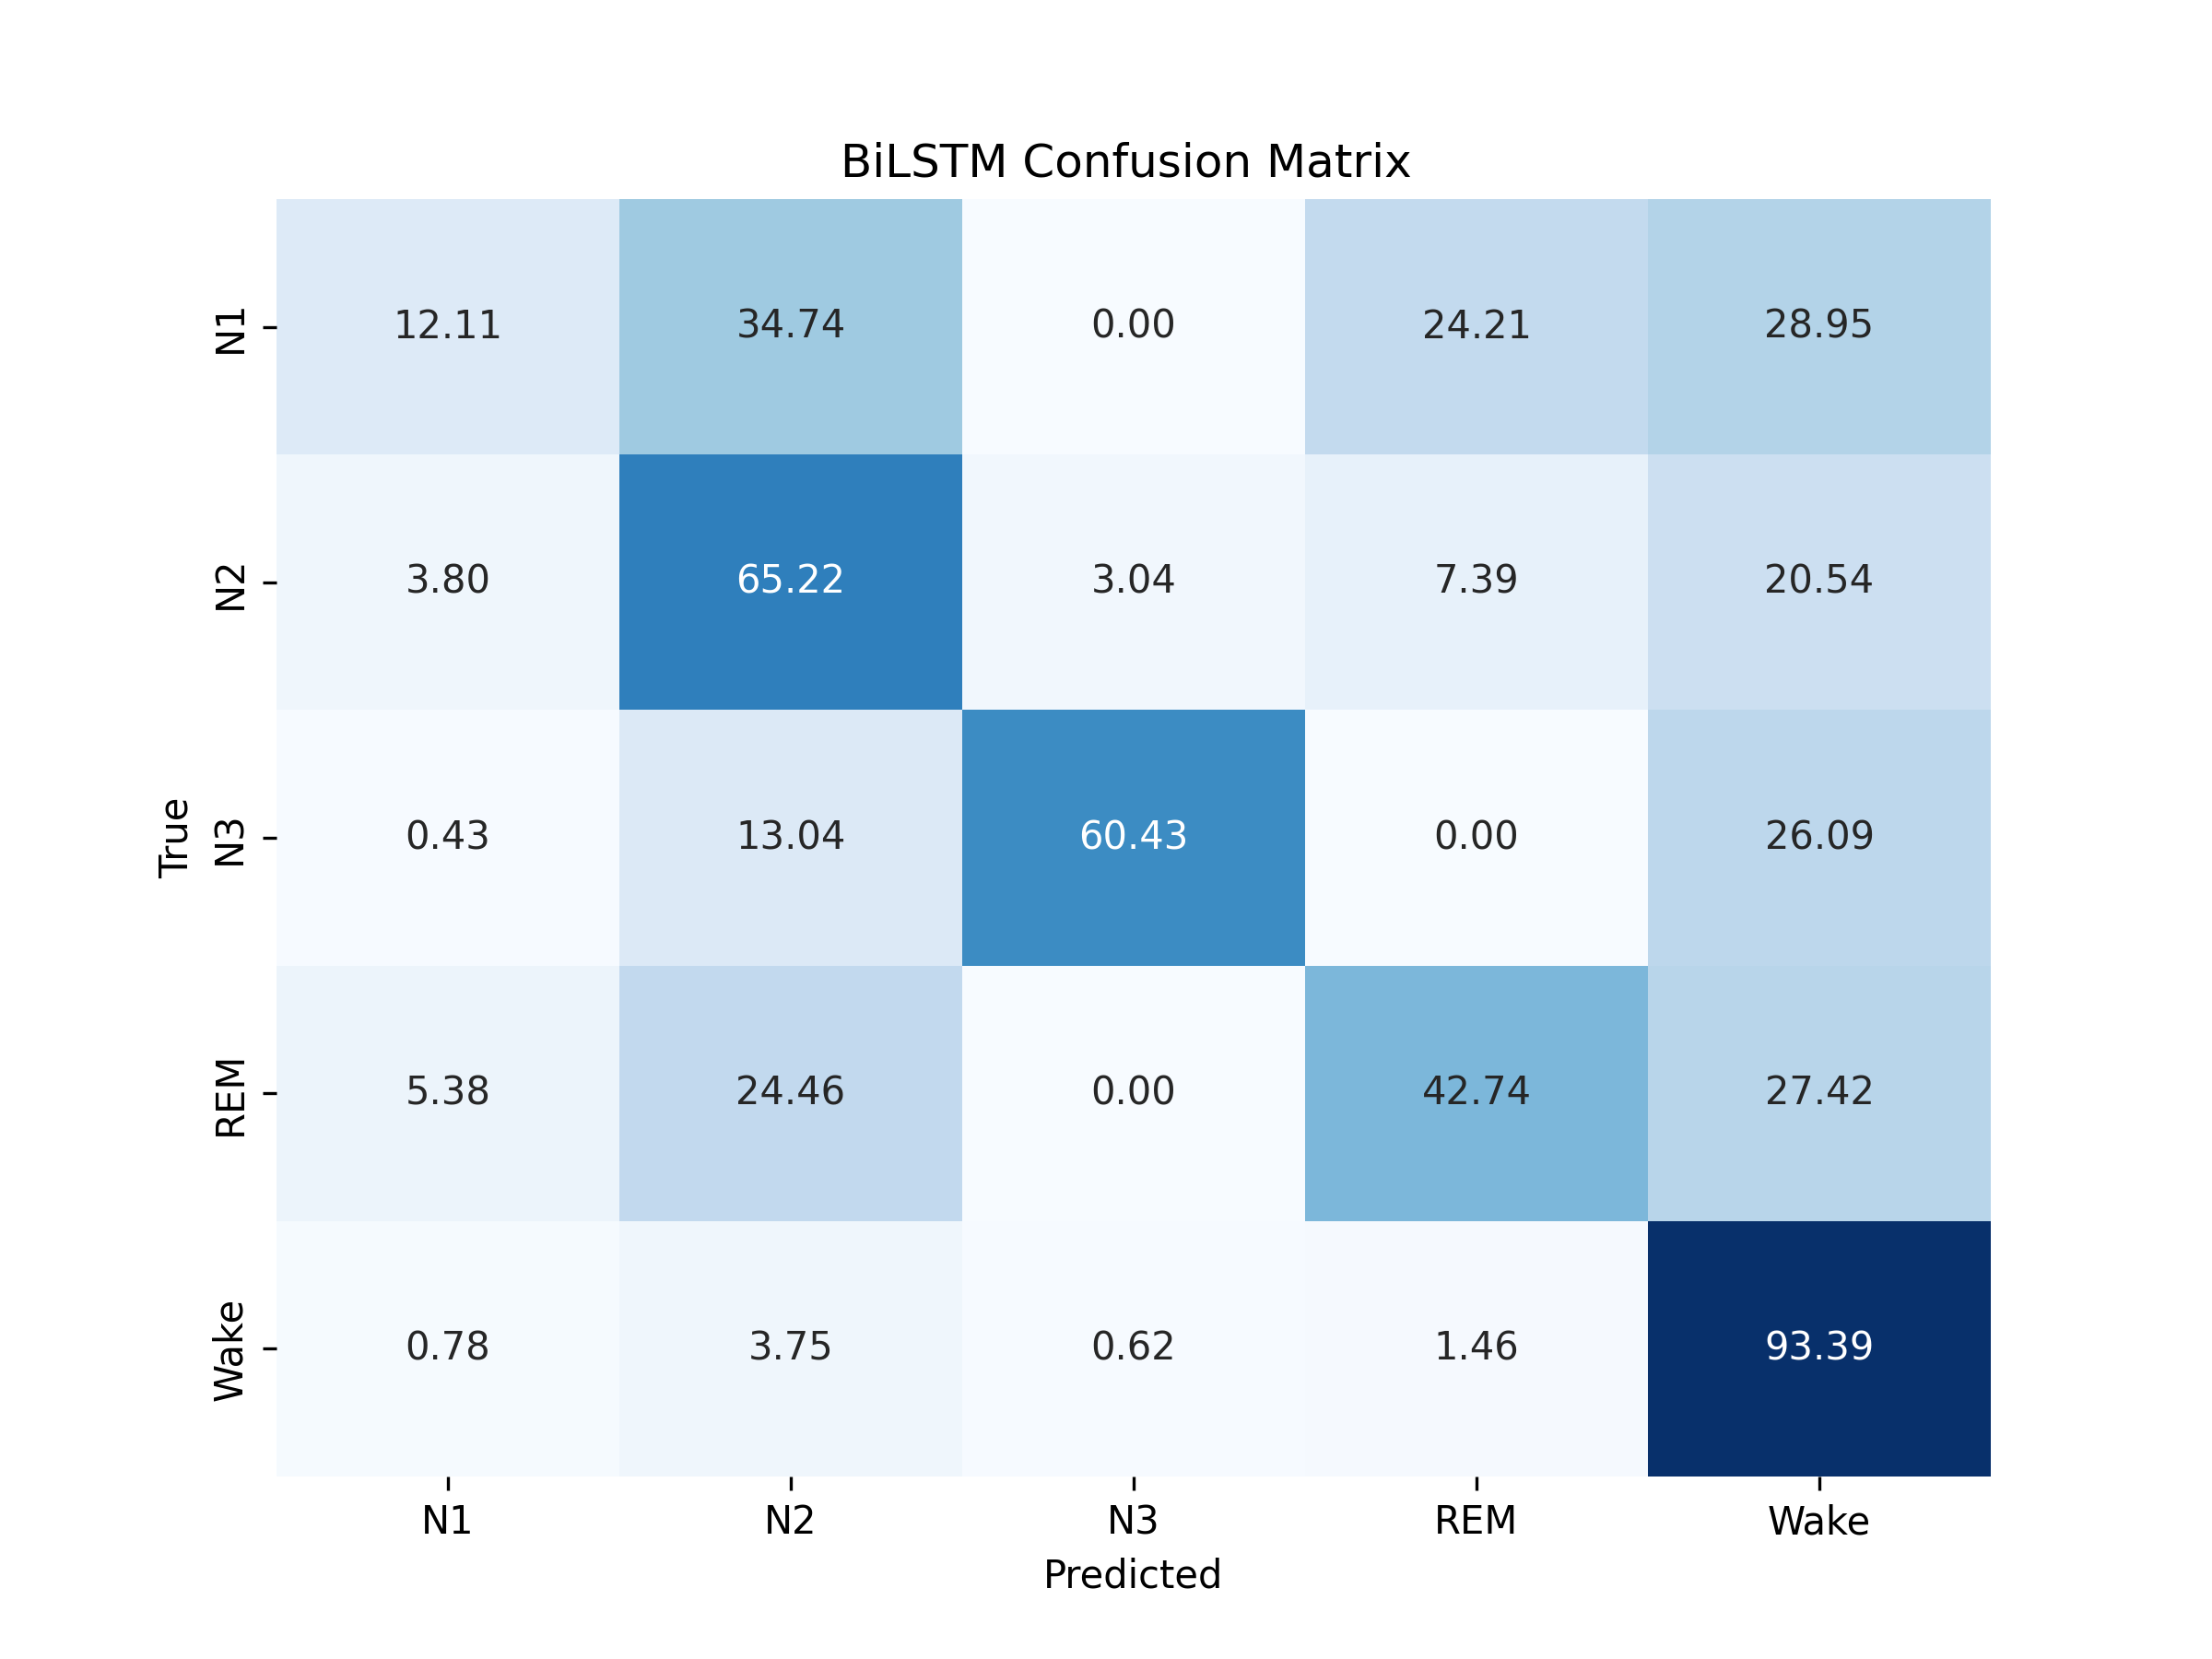
\includegraphics[width=\linewidth]{img/paper_2/BiLSTM_cm.png}
		\caption{BiLSTM Confusion Matrix}
		\label{fig:bilstm_cm}
	\end{minipage}
\end{figure}



\section{Comparison of Results}



This section presents a comparative analysis of multiple machine learning models applied to the sleep stage classification problem. The evaluation metrics considered include accuracy, weighted and macro averages of precision, recall, and F1-score.

\subsection{Testing  Models Overview}



\begin{table}[H]
	\centering
	\caption{Performance Comparison of Models}
	\label{tab:metrics_summary}
	\begin{tabular}{lcccccc}
		\hline
		\textbf{Model} & \textbf{Accuracy} & \textbf{Wgt. F1} & \textbf{Macro F1} & \textbf{Macro Prec.} & \textbf{Macro Rec.} \\
		\hline
		Random Forest          & \textbf{0.843} & \textbf{0.823} & 0.641 & \textbf{0.901} & 0.558 \\
		XGBoost                & \textbf{0.854} & \textbf{0.843} & 0.644 & \textbf{0.776} & 0.599 \\
		Neural Network         & \textbf{0.777} & \textbf{0.750} & 0.487 & 0.567 & 0.452 \\
		LSTM                   & \textbf{0.800} & \textbf{0.785} & 0.461 & 0.499 & 0.436 \\
		BiLSTM                 & \textbf{0.811} & \textbf{0.803} & 0.472 & 0.494 & 0.457 \\
		RNN                    & 0.706 & 0.690 & 0.332 & 0.381 & 0.345 \\
		AdaBoost               & 0.312 & 0.353 & 0.273 & 0.323 & 0.399 \\
		KNN (with PCA)         & 0.194 & 0.189 & 0.272 & 0.296 & 0.359 \\
		\hline
	\end{tabular}
\end{table}


\subsection{Discussion}

Among all the models tested, the \textbf{XGBoost classifier} achieved the highest overall accuracy (0.854) and weighted F1-score (0.843), narrowly outperforming the Random Forest model. While Random Forest achieved a slightly higher macro precision (0.901 vs. 0.776), its recall across minority classes such as N1 and REM was relatively lower.

The deep learning-based models (LSTM and BiLSTM) followed closely behind the tree-based models, with BiLSTM slightly outperforming LSTM (macro F1 of 0.472 vs. 0.461). The \textbf{Neural Network model}, although simpler, showed moderate performance (macro F1 of 0.487), better than AdaBoost and KNN.

\textbf{K-Nearest Neighbors (KNN)} and \textbf{AdaBoost} performed poorly in this context. KNN failed to handle the class imbalance effectively, leading to very low overall accuracy (0.194). AdaBoost performed slightly better but still struggled to generalize, especially for majority class (Wake) classification.

The \textbf{RNN model} had the lowest macro F1-score (0.332) among deep models, indicating potential vanishing gradient issues or insufficient context capture compared to LSTM-based architectures.

\subsection{Conclusion}

Tree-based ensemble methods (XGBoost, Random Forest) consistently outperformed others across all key metrics. Deep learning models, especially BiLSTM, offer competitive alternatives with relatively strong performance. Simpler models like KNN and AdaBoost underperform and are not suitable for this imbalanced multiclass classification task without further tuning or class balancing.



\subsection{Comparison Plot}
The following plot presents a comparison of the accuracy scores for different models.
\begin{figure}[H]
	\centering
	\begin{minipage}{0.48\textwidth}
		\centering
		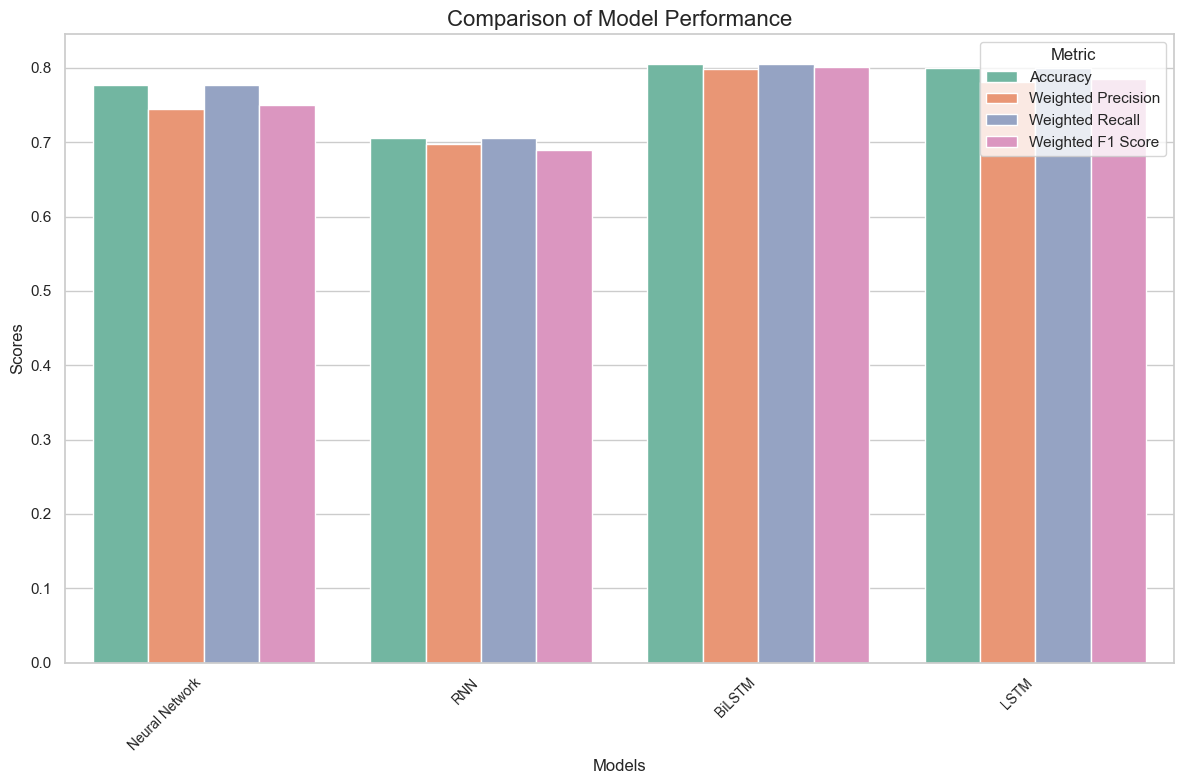
\includegraphics[width=\linewidth]{img/paper_2/Comparision Plot.png}
		\caption{Accuracy Comparison Across All Models}
		\label{fig:accuracy_comparison}
	\end{minipage}
	\hfill
	\begin{minipage}{0.48\textwidth}
		\centering
		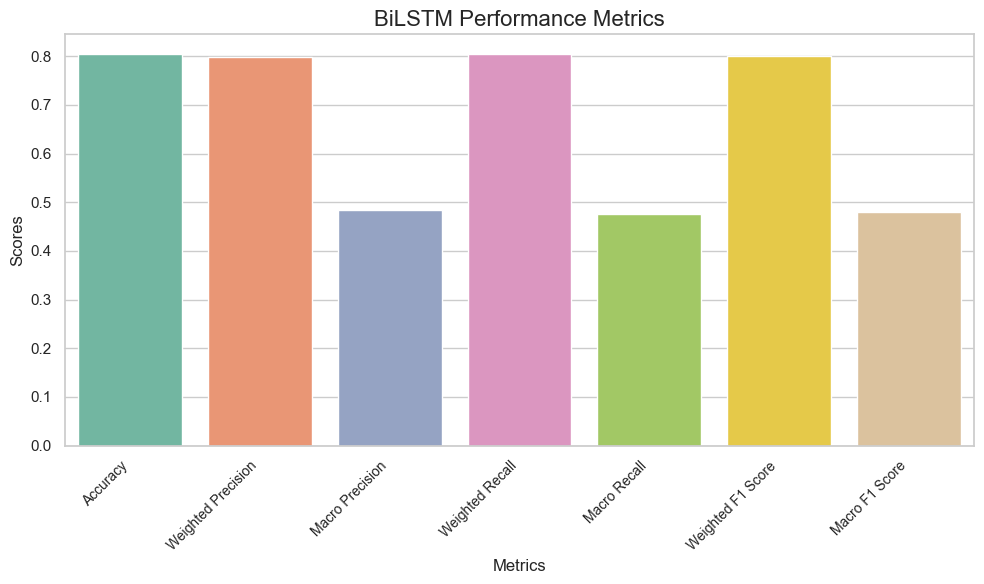
\includegraphics[width=\linewidth]{img/paper_2/BILSTM.png}
		\caption{Bi-LSTM Model Performance}
		\label{fig:bilstm_performance}
	\end{minipage}
	
	\vspace{0.5cm}
	
	\begin{minipage}{0.48\textwidth}
		\centering
		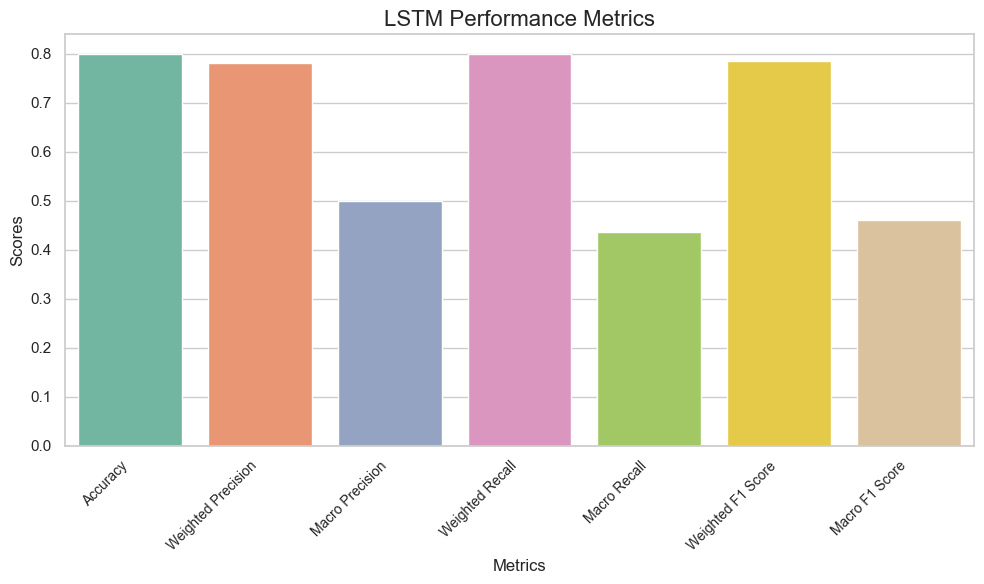
\includegraphics[width=\linewidth]{img/paper_2/LSTM.png}
		\caption{LSTM Model Performance}
		\label{fig:lstm_performance}
	\end{minipage}
	\hfill
	\begin{minipage}{0.48\textwidth}
		\centering
		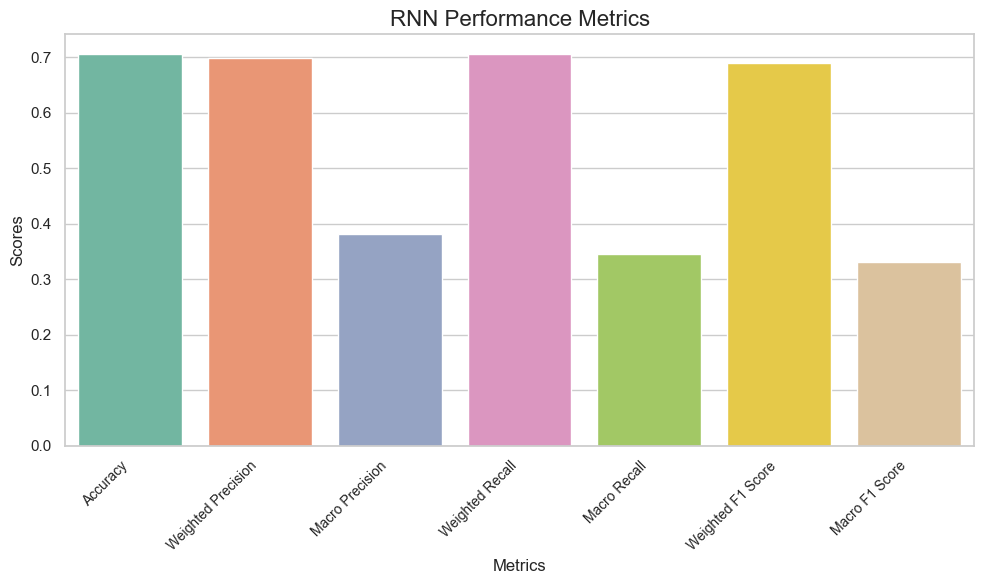
\includegraphics[width=\linewidth]{img/paper_2/RNN.png}
		\caption{RNN Model Performance}
		\label{fig:rnn_performance}
	\end{minipage}
\end{figure}

\begin{figure}[H]
	\centering
	\begin{minipage}{0.48\textwidth}
		\centering
		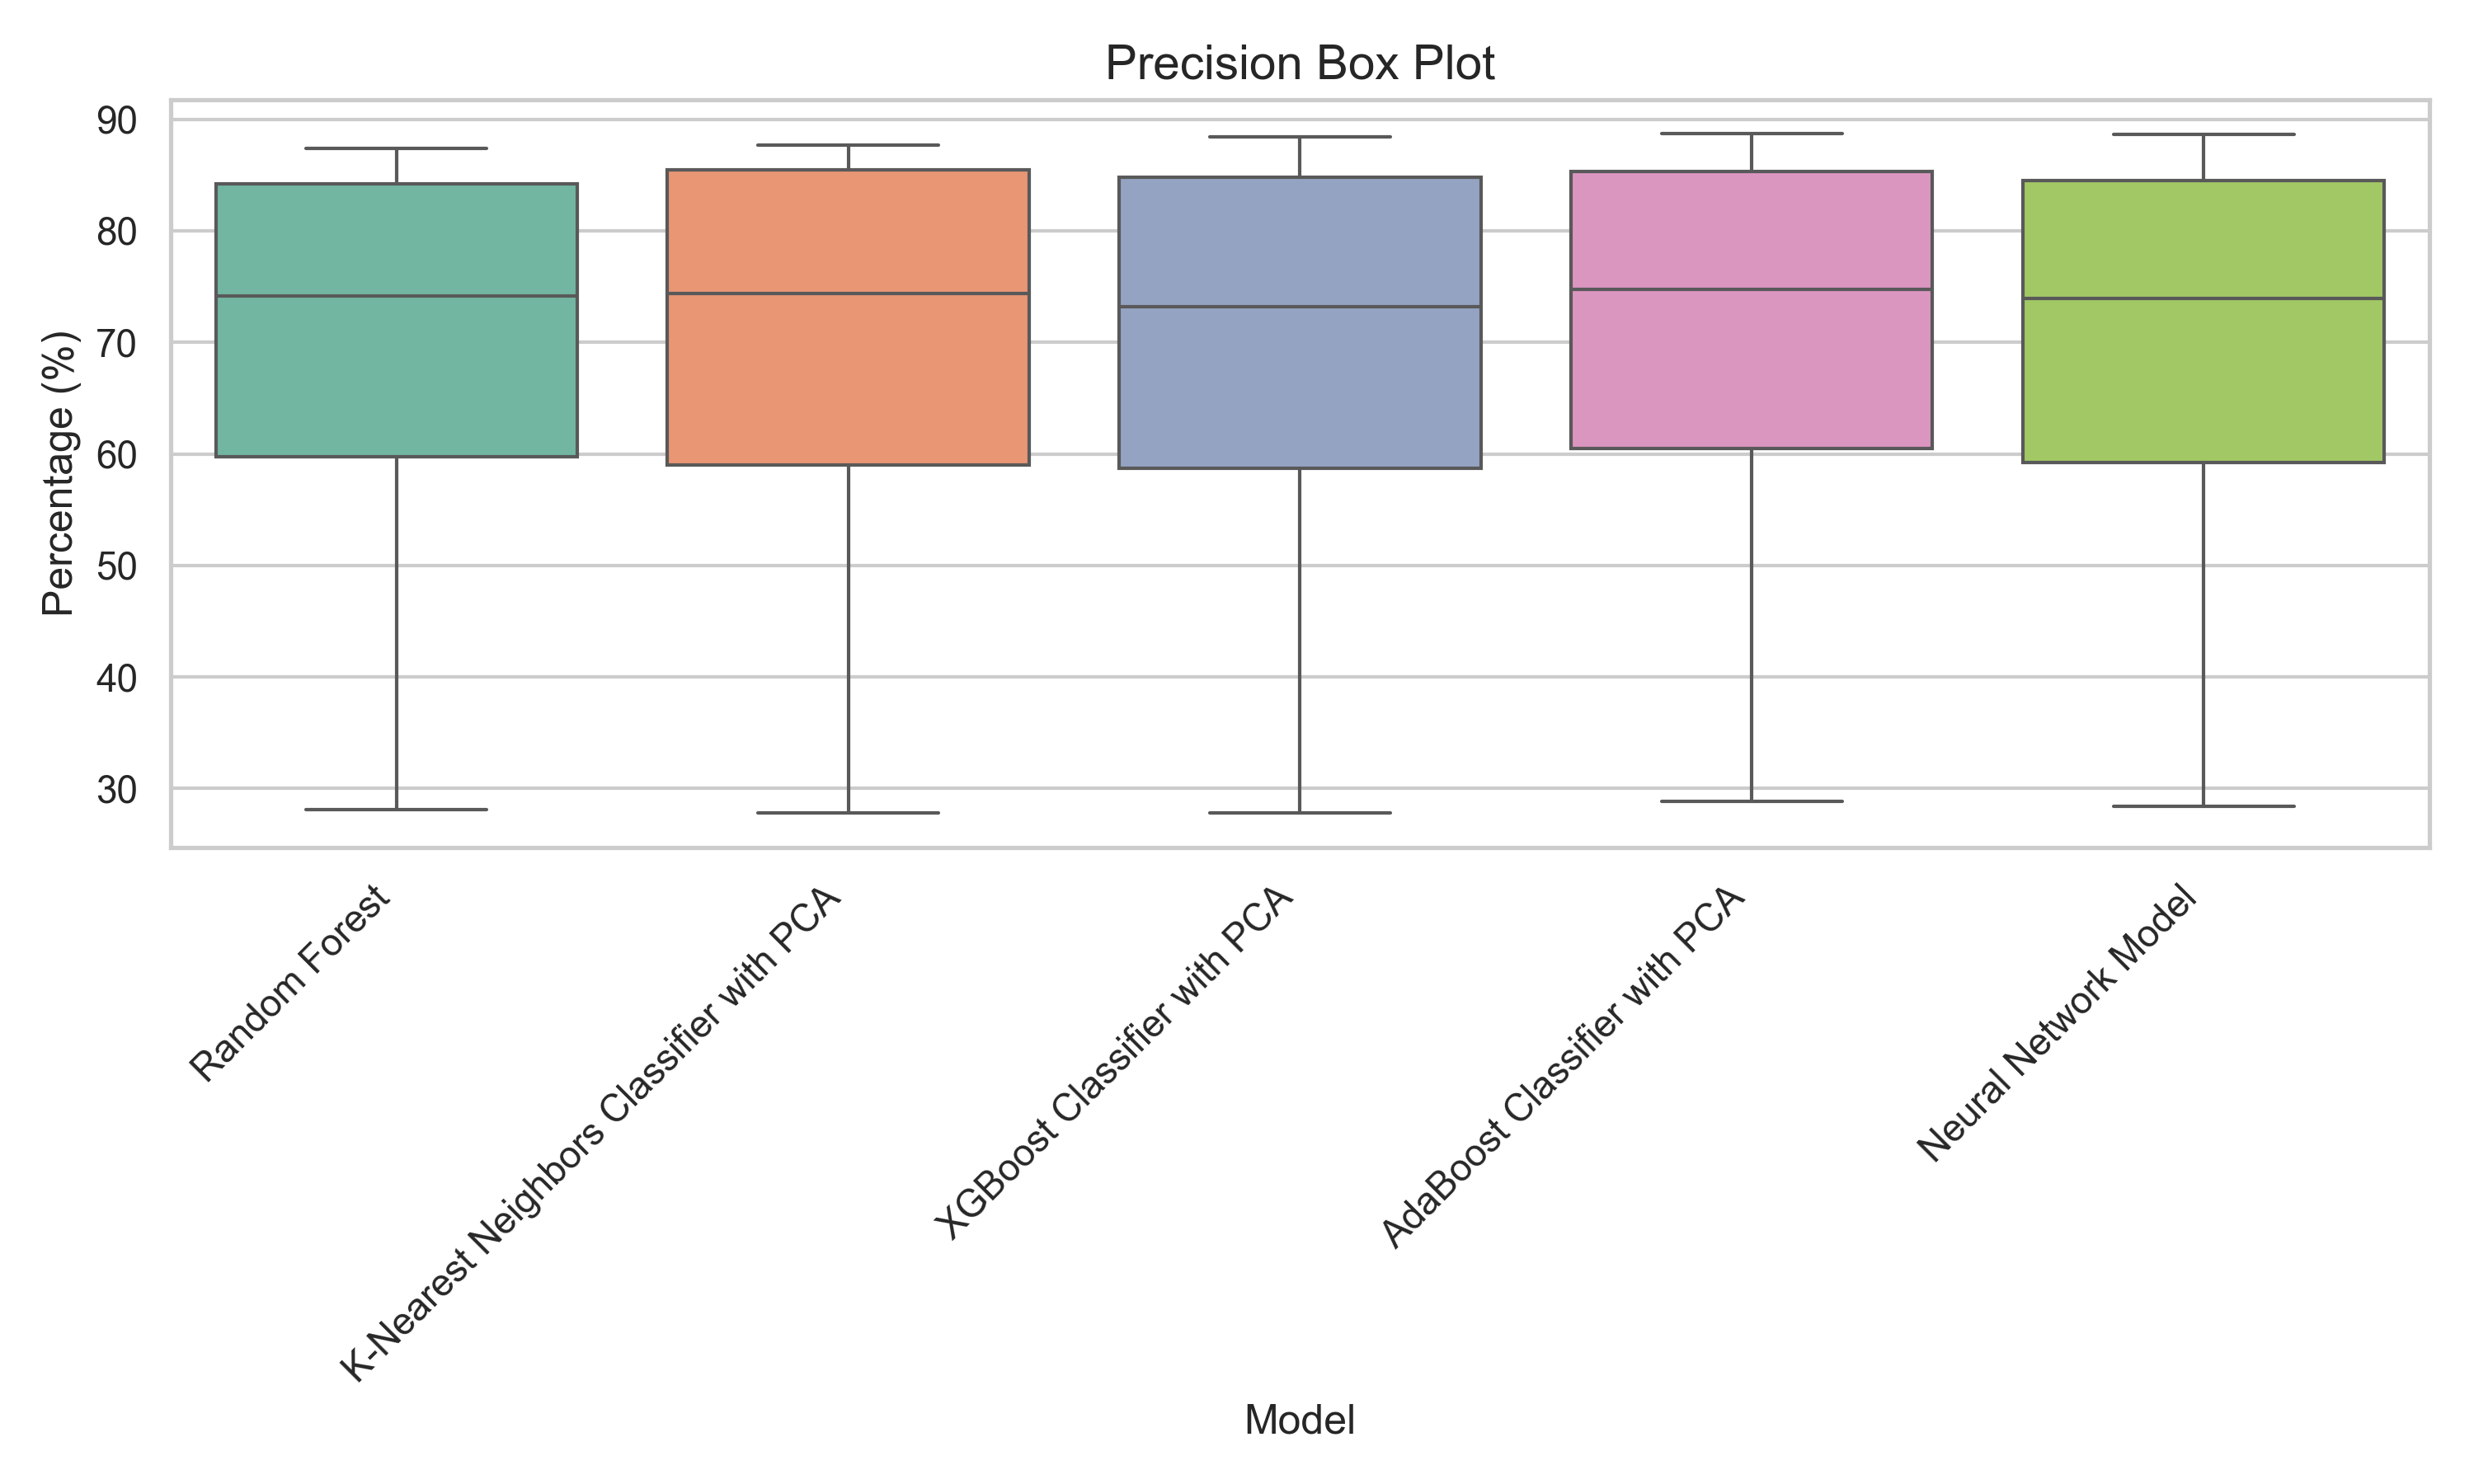
\includegraphics[width=\linewidth]{img/paper_2/Precision_box_plot}
		\caption{Box Plot of ML Precision Across Models}
		\label{fig:precisionboxplot}
	\end{minipage}
	\hfill
	\begin{minipage}{0.48\textwidth}
		\centering
		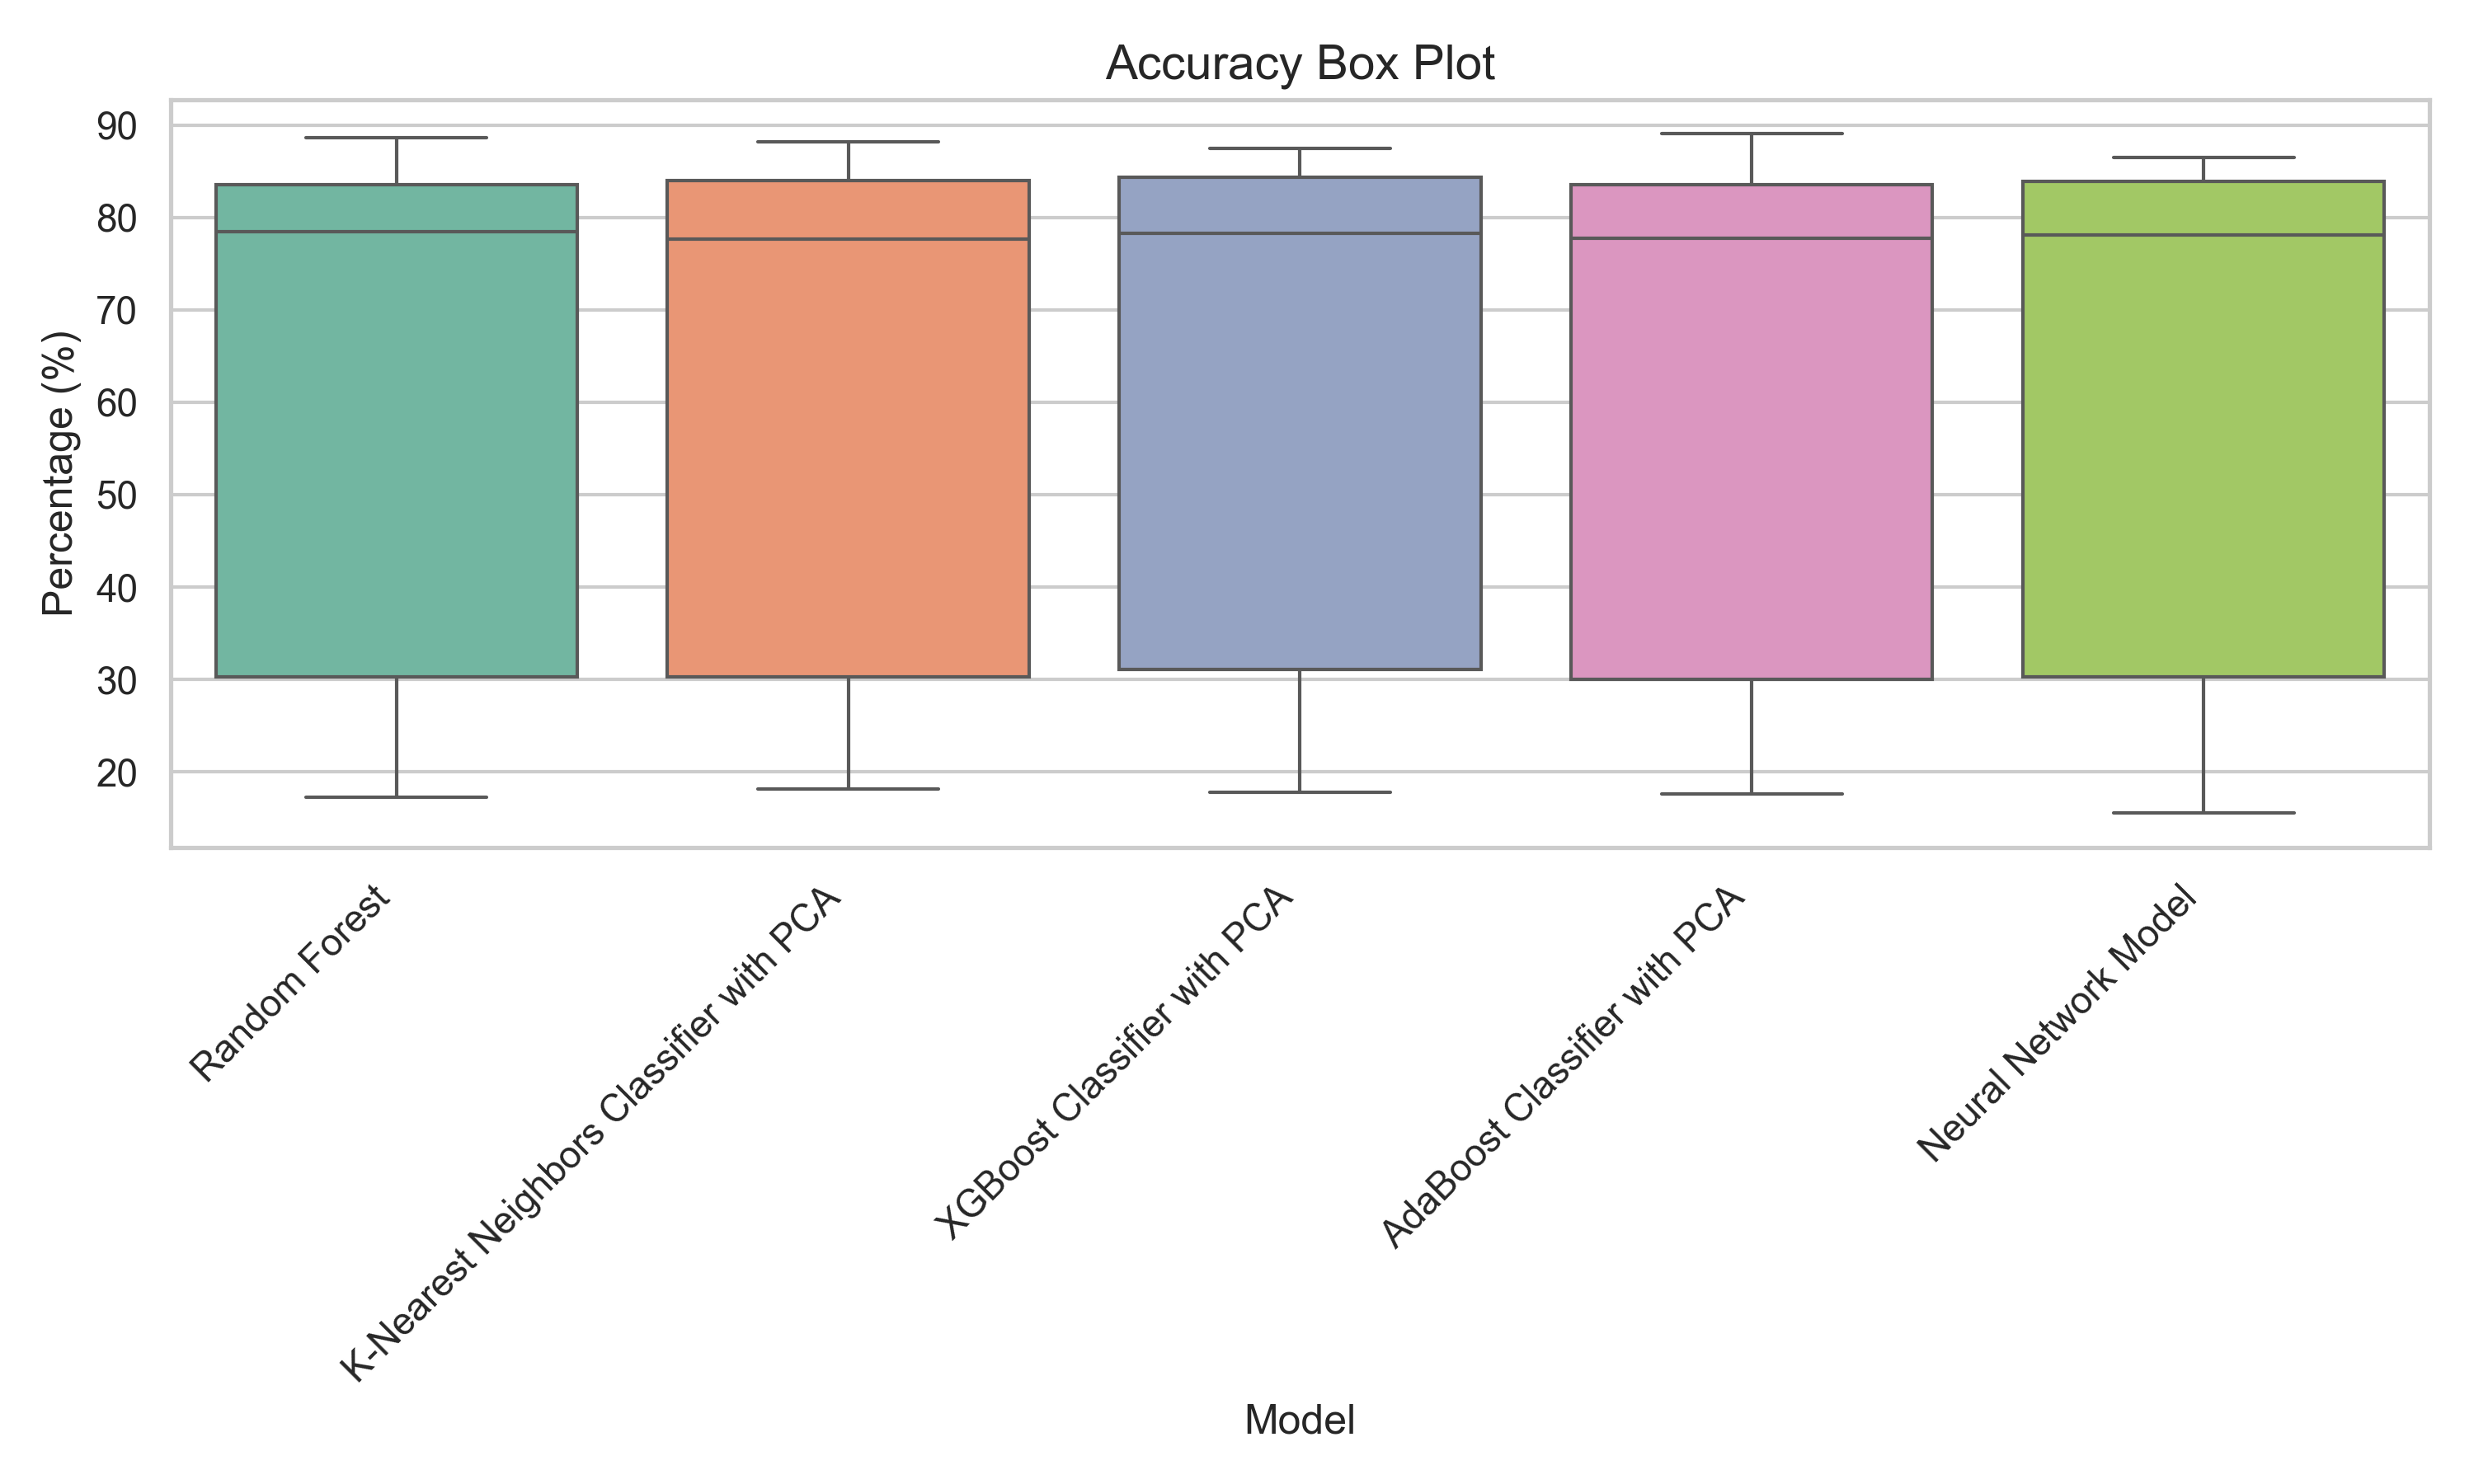
\includegraphics[width=\linewidth]{img/paper_2/Accuracy_box_plot}
		\caption{Box Plot of ML Accuracy Across Models}
		\label{fig:accuracyboxplot}
	\end{minipage}
\end{figure}


\chapter{SleepGCN-Transformer: A Hybrid Graph-Convolutional and Transformer Network for Sleep Stage Classification}
\label{chapter_paper3}

\section{Methodology}



The SleepGCN-Transformer is a hybrid deep learning framework designed for accurate sleep stage classification by combining the strengths of Graph Convolutional Networks (GCNs) and Transformer architectures. This model is trained on the Sleep-EDF dataset, utilizing four critical physiological signal channels: EEG Fpz-Cz, EEG Pz-Oz, EOG (horizontal), and submental EMG.


\begin{figure}
	\centering
	\includegraphics[width=0.8\linewidth]{"img/paper_3/hypnogram sleep stage transition"}
	\caption{Hypnogram With Transition Heighlights }
	\label{fig:hypnogram-sleep-stage-transition}
\end{figure}




In this architecture, GCNs are employed to capture spatial relationships between the multimodal input signals, while the Transformer encoder is tasked with modeling the temporal dependencies across time sequences. This dual approach ensures that both spatial and sequential dynamics are effectively learned.

Experimental results confirm the effectiveness of the model, achieving an accuracy of 93.12\% on the training set and 93.04\% on the validation set. To address class imbalance—particularly the underrepresentation of certain sleep stages—the model incorporates Focal Loss, which emphasizes harder-to-classify samples during training.

Further analysis of feature importance revealed that the EMG and EEG Pz-Oz channels play a significant role in predicting sleep stages. This methodological framework not only enhances classification performance but also supports the integration of explainable AI techniques, contributing to the development of interpretable tools for clinical sleep analysis and decision-making.

\begin{figure}
	\centering
	\includegraphics[width=.9\linewidth]{"img/paper_3/Graph Convolution Neural Network -SleepGCN_Transformer Architechture"}
	\caption{Proposed Architecture of the sleep GCN- Transformer Architecture}
	\label{fig:graph-convolution-neural-network--sleepgcntransformer-architechture}
\end{figure}



\section{Dataset and Implementation Environment}

Our experiments were conducted using the publicly available Sleep-EDF dataset, which is widely utilized for sleep stage classification research. The dataset can be accessed at \url{https://physionet.org/content/sleep-edfx/1.0.0/}, and it includes EEG recordings labeled with corresponding sleep stages, enabling effective supervised learning.

The implementation was carried out in Python 3.13.1 using the PyTorch deep learning framework. Development was performed in Visual Studio Code (VS Code) on a machine powered by the Apple M1 chip, utilizing both CPU and Metal acceleration capabilities for training efficiency.

For version control and collaborative development, we used GitHub to manage our codebase. The repository containing our source code is publicly available at \url{https://github.com/tanmay007thor/GCN}.

The source code of this research is licensed under the Apache License 2.0, which allows for open use and distribution. The license details are available at \url{http://www.apache.org/licenses/}.

To support data processing, model training, and evaluation, we relied on several key Python libraries. The primary libraries and their versions used in our project include: NumPy 2.2.2, Pandas 2.2.3, Scikit-learn 1.6.1, SciPy 1.15.1, Matplotlib 3.10.0, Seaborn 0.13.2, PyTorch 2.6.0, Torch Geometric 2.6.1, NetworkX 3.4.2, and MNE 1.9.0. This software environment ensured a reliable, efficient, and reproducible workflow throughout our research.



\section{Preprocessing Techniques}
\begin{figure}[H]
	\centering
	\begin{minipage}{0.48\textwidth}
		\centering
		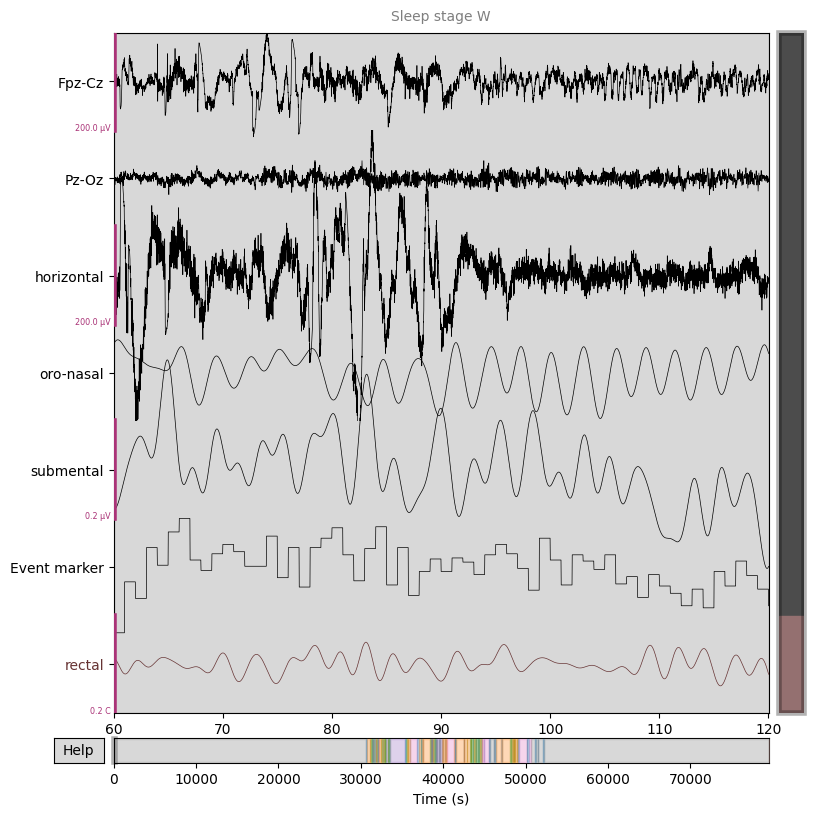
\includegraphics[width=\linewidth]{img/paper_3/Signals}
		\caption{Raw signal channels from the Sleep-EDF dataset}
		\label{fig:raw_signals}
	\end{minipage}
	\hfill
	\begin{minipage}{0.48\textwidth}
		\centering
		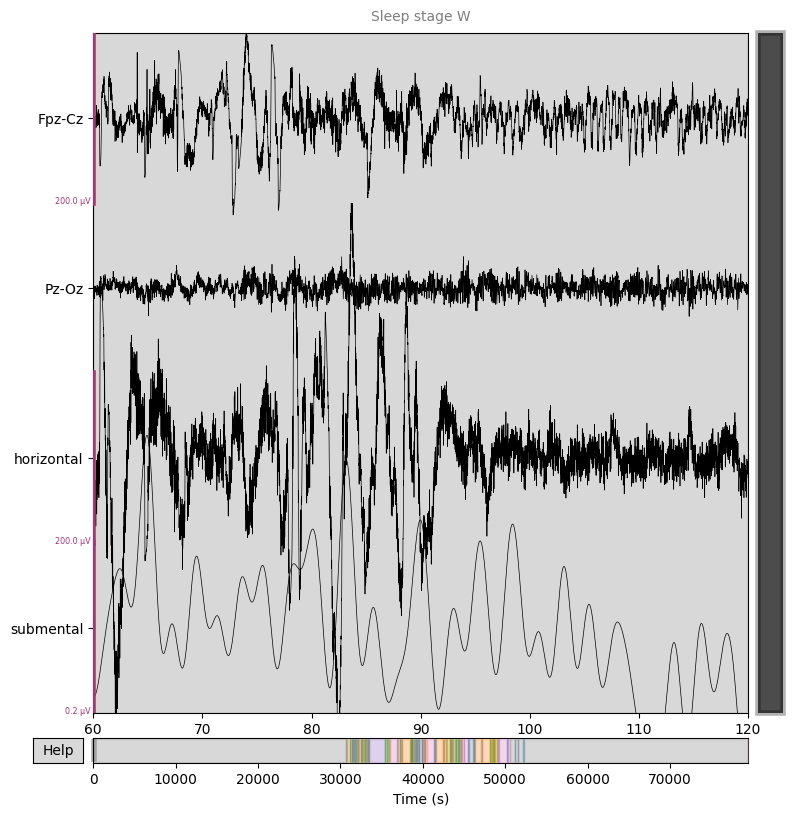
\includegraphics[width=\linewidth]{img/paper_3/filtered chanels}
		\caption{Preprocessed and filtered signal channels}
		\label{fig:filtered_signals}
	\end{minipage}
\end{figure}


\subsection{Data Information}

The Sleep-EDF dataset comprises multichannel physiological signals, including EEG, EOG, EMG, nasal airflow, and temperature, each accompanied by event markers. These signals are recorded over 60-second intervals, with frequency content varying between 60 and 120 Hz. The dynamic nature of these signals introduces significant variability, making it challenging to identify consistent patterns for classification. Such rapid fluctuations can increase the likelihood of misclassification. Furthermore, the dataset presents several challenges such as high-frequency noise, class imbalance (notably a dominance of the Wake stage), and a substantial number of time steps—approximately 100 time steps per second—adding complexity to the task of modeling sleep stages.

\subsection{Preprocessing Pipeline}

To address these challenges, we developed a comprehensive preprocessing pipeline focused on selecting the most informative channels and reducing irrelevant data. Initially, we discarded several channels that were found to contribute minimally to sleep stage classification. The retained signals included the EEG channels (Fpz-Cz and Pz-Oz), the horizontal EOG channel (to track eye movement), and the submental EMG channel (for monitoring chin muscle activity).

Each sleep stage in the dataset was mapped to a simplified class label to consolidate similar stages and reduce classification ambiguity. Table~\ref{tab:sleep_stage_mapping} presents the sleep stage-to-class mapping:

\begin{table}[H]
	\centering
	\caption{Sleep Stage Mapping}
	\label{tab:sleep_stage_mapping}
	\begin{tabular}{llc}
		\hline
		\textbf{Sleep Stage} & \textbf{Label} & \textbf{Mapped Class} \\
		\hline
		Wake                & 0 & 0 \\
		Stage 1             & 1 & 1 \\
		Stage 2             & 2 & 2 \\
		Stage 3             & 3 & 3 \\
		Stage 4             & 4 & 3 \\
		REM                 & 5 & 4 \\
		\hline
	\end{tabular}
\end{table}

The preprocessing begins with reading the EDF recordings and assigning sleep labels based on the mapped classes. Subsequently, we applied a bandpass filter to isolate relevant frequency ranges. Specifically, the signal was filtered to retain only the 0.3–30 Hz band using the firwin filter design, effectively removing noise and irrelevant frequencies outside this band. Though not a standard approach, this customized filtering was found to be better suited to our specific dataset and classification task.

We then segmented the signals into fixed-length epochs of 30 seconds. The final preprocessed data was shaped into a three-dimensional format: $(X, 4, 3000)$, where $X$ is the number of epochs (samples), $4$ is the number of selected channels, and $3000$ corresponds to the number of time steps per epoch.

\subsection{Filtering Method}

The filtering was implemented using a windowed time-domain design via the firwin method. A Hamming window was employed, configured with a 0.0194 passband ripple and 53 dB stopband attenuation. The filter characteristics were as follows: lower passband edge at 0.30 Hz, lower transition bandwidth of 0.30 Hz (with a $-6$ dB cutoff at 0.15 Hz), upper passband edge at 30.00 Hz, and an upper transition bandwidth of 7.50 Hz (with a $-6$ dB cutoff at 33.75 Hz). These settings were carefully chosen to preserve the signal components relevant to sleep staging while minimizing noise.























\section{Model Architecture and Learning Framework}

To extract spatial features from the multi-channel data, we construct a graph using the four selected channels, where each channel acts as a node and the edges represent their interrelationships. These edges are weighted based on prior literature and empirical observations, assigning higher importance to EEG channels due to their strong influence on sleep stage detection. In contrast, connections involving EMG and EOG are assigned lower weights, as EOG shows weaker correlations. Although assigning self-loop weights is possible, we chose not to include them in this implementation.


\begin{figure}
	\centering
	\includegraphics[width=.9\linewidth]{"img/paper_3/Graph Convolution Neural Network -SleepGCN_Transformer Architechture"}
	\caption{Proposed Architecture of the sleep GCN- Transformer Architecture}
	\label{fig:graph-convolution-neural-network--sleepgcntransformer-architechture}
\end{figure}

The final dataset comprises 11,076 samples, structured as \texttt{Data(x=[3000, 4], edge\_index=[2, 12], edge\_attr=[12], y=[1])}. Here, \texttt{x} represents the time-series data with 3,000 time steps across 4 channels, \texttt{edge\_index} defines the graph connectivity, \texttt{edge\_attr} contains the edge weights, and \texttt{y} denotes the sleep stage label. This dataset is created using the \texttt{SleepEEGDataset} class and is designed to effectively model spatial dependencies across EEG, EMG, and EOG signals, thereby enhancing sleep stage classification performance.


\begin{figure}
	\centering
	\includegraphics[width=0.7\linewidth]{"img/paper_3/Graph Weightage"}
	\caption{Graph Dataset Creation}
	\label{fig:graph-weightage}
\end{figure}

\subsection{GCN Architecture}

To capture spatial dependencies across the selected EEG, EMG, and EOG channels, we incorporate a Graph Convolutional Network (GCN) into our model. Each sample is structured as a graph with four nodes—corresponding to the four selected channels—and each node contains a time series of 3,000 time steps. The dataset comprises 11,076 such graph-based samples.

The GCN consists of five identical graph convolution layers. The initial input has a shape of (4, 3000), which is projected to (4, 256) after the first graph convolution. Each layer includes batch normalization (256 units), followed by a ReLU activation function and a dropout of 0.1. After the final GCN layer, we apply global mean pooling to obtain a graph-level representation.

The propagation rule used in each GCN layer is given by:

\begin{equation}
	H^{(l+1)} = \sigma\left(\tilde{D}^{-1/2} \tilde{A} \tilde{D}^{-1/2} H^{(l)} W^{(l)}\right)
\end{equation}

\begin{itemize}
	\item $H^{(l)} \in \mathbb{R}^{N \times D}$ is the feature matrix at layer $l$, where $N$ is the number of nodes and $D$ is the feature dimension.
	\item $\tilde{A} = A + I$ is the adjacency matrix with self-loops.
	\item $\tilde{D}$ is the degree matrix corresponding to $\tilde{A}$.
	\item $W^{(l)}$ is the learnable weight matrix for layer $l$.
	\item $\sigma$ denotes a non-linear activation function, typically ReLU.
\end{itemize}

The simplified form for one GCN layer operation is:

\begin{equation}
	X' = \sigma\left(\tilde{D}^{-1/2} \tilde{A} \tilde{D}^{-1/2} X W\right)
\end{equation}

To aggregate node features into a graph-level embedding, we use global mean pooling:

\begin{equation}
	x = \frac{1}{|V|} \sum_{v \in V} h_v
\end{equation}

\begin{itemize}
	\item $V$ is the set of nodes in the graph.
	\item $h_v$ is the feature vector of node $v$.
	\item $x$ is the pooled feature vector representing the entire graph.
\end{itemize}

We apply standard activation and normalization functions during training:

\begin{equation}
	\text{ReLU}(x) = \max(0, x)
\end{equation}

\begin{equation}
	\text{softmax}(x_i) = \frac{e^{x_i}}{\sum_j e^{x_j}}
\end{equation}

\begin{equation}
	x'' = \frac{x' - \mu}{\sigma}
\end{equation}

\begin{itemize}
	\item $\mu$ is the mean of $x'$.
	\item $\sigma$ is the standard deviation of $x'$.
	\item $x''$ is the normalized feature representation.
\end{itemize}


\subsection{Transformer Architecture}

To capture temporal dependencies in the input signal, we utilize a Transformer encoder comprising two stacked layers. Initially, the input is projected into a continuous vector space using an embedding layer. Since Transformers lack inherent mechanisms for handling sequential order, positional encodings are added to preserve time-step information. 

Following embedding and encoding, we use multi-head self-attention to allow the model to focus on different aspects of the signal simultaneously. The attention outputs are concatenated and passed through a feedforward network with dropout regularization. Finally, a fully connected classifier outputs logits for four-class sleep stage classification.

The operations within the Transformer encoder are summarized using the following equations:
\subsection{Transformer: Key Components and Equations}

\begin{itemize}
	\item \textbf{Input Embedding:} Maps input tokens into a continuous vector space.
	\begin{equation}
		X_{\text{embed}} = X W_{\text{embed}}
	\end{equation}
	
	\item \textbf{Positional Encoding:} Adds sequence order information using sine and cosine functions.
	\begin{equation}
		PE(\text{pos}, 2i) = \sin\left(\frac{\text{pos}}{10000^{2i/d}}\right)
	\end{equation}
	\begin{equation}
		PE(\text{pos}, 2i+1) = \cos\left(\frac{\text{pos}}{10000^{2i/d}}\right)
	\end{equation}
	
	\item \textbf{Query, Key, and Value Computation:} Core of attention mechanism, derived from input.
	\begin{equation}
		Q = XW_q,\quad K = XW_k,\quad V = XW_v
	\end{equation}
	
	\item \textbf{Scaled Dot-Product Attention:} Computes weighted output of values using attention scores.
	\begin{equation}
		H_1 = \text{softmax}\left(\frac{QK^T}{\sqrt{d_k}}\right) V
	\end{equation}
	
	\item \textbf{Multi-Head Attention:} Combines multiple attention outputs for diverse feature learning.
	\begin{equation}
		H = \text{Concat}(H_1, H_2, ..., H_h) W_0
	\end{equation}
\end{itemize}









































\subsection{Training Pipeline}

\textbf{Fully Connected Layer:}  
The final stage of the model includes a linear transformation layer that maps a 256-dimensional input vector to 5 output logits, corresponding to the five target sleep stages. This transformation enables direct classification output.

\subsubsection*{Why Focal Loss Instead of Standard Cross-Entropy?}

Standard cross-entropy loss treats all training samples equally, which can lead to a bias toward majority classes in imbalanced datasets. In such settings, the model tends to suppress the prediction of minority classes, resulting in poor generalization. Focal Loss addresses this by dynamically adjusting the contribution of each sample based on the confidence of its prediction. This mechanism reduces the influence of well-classified samples and increases the focus on harder, misclassified instances.

Focal Loss introduces two key parameters: the focusing parameter $\gamma$, which controls the down-weighting of easy examples, and the class weighting factor $\alpha$, which helps balance class frequencies during training. These features make Focal Loss particularly effective for classification tasks involving significant class imbalance.

\subsubsection*{Focal Loss Formulation}

The Focal Loss is mathematically expressed as:

\[
FL(p_t) = -\alpha(1 - p_t)^{\gamma} \log(p_t)
\]

Here, $p_t$ denotes the predicted probability for the target class, $\alpha$ is the balancing factor to compensate for class imbalance, and $\gamma$ adjusts the focus on misclassified examples.

To enhance numerical stability and improve generalization, label smoothing is applied:

\[
y_{\text{smooth}} = y(1 - \epsilon) + \frac{\epsilon}{C}
\]

This prevents issues such as $\log(0)$ and ensures a more stable optimization process. The combined implementation of Focal Loss with label smoothing can be written in a PyTorch-like style as:

\[
L = \alpha(1 - p)^{\gamma} \left( - y_{\text{smooth}} \log(p) \right)
\]

\subsubsection*{Learning Rate Scheduling}

The learning rate is a critical hyperparameter that governs the pace of model updates during training. A high learning rate may cause divergence, while a low learning rate can result in slow convergence or suboptimal local minima. Therefore, adaptive learning rate scheduling is essential for efficient training.

CosineAnnealingLR is used as the scheduling strategy, as it provides a smooth and gradual reduction in the learning rate. It allows for large updates in the early stages of training and fine-tuning in later stages, thereby helping the model generalize better. The learning rate at each epoch $t$ is computed using the following cosine annealing formula:

\[
\eta_t = \eta_{\min} + \frac{1}{2} (\eta_{\max} - \eta_{\min}) \left( 1 + \cos \left( \frac{\pi T_{\text{cur}}}{T_{\text{max}}} \right) \right)
\]

In this equation, $\eta_t$ is the learning rate at epoch $t$, $\eta_{\min}$ and $\eta_{\max}$ are the minimum and maximum learning rates respectively, $T_{\text{cur}}$ is the current epoch, and $T_{\text{max}}$ is the total number of epochs.

\subsubsection*{Training Methodology Overview}

The training pipeline is encapsulated within a dedicated class named \texttt{SleepTrainer}, which manages model training, validation, and optimization. The training process begins with the computation of class weights to address data imbalance. The model is then trained using mini-batch gradient descent, where each batch is used to compute the loss and update the model parameters accordingly. Performance is periodically evaluated on a separate validation set, and the learning rate is adjusted dynamically using the scheduler.

\subsubsection*{Hyperparameters Used}

The training setup uses a batch size of 32 and an initial learning rate of 0.0003. The optimizer of choice is AdamW, with a weight decay of $1 \times 10^{-4}$ to prevent overfitting. Training is conducted for 20 epochs, and the CosineAnnealingLR scheduler is applied to adjust the learning rate over time. This configuration ensures smooth convergence and robust generalization.

\subsubsection*{Handling Class Imbalance}

EEG sleep stage data is inherently imbalanced, with some stages appearing far more frequently than others. To address this, class weights are computed and incorporated into the loss function. The weighting formula is given by:

\[
w_c = \left( \frac{\text{Total Samples}}{\text{Class Count} + 1} \right)^{0.5}
\]

This formulation ensures that less frequent classes receive proportionally higher weights, encouraging the model to give them more attention during training. These computed weights are then integrated directly into the Focal Loss function to balance the influence of each class.

\subsubsection*{Testing Data Distribution Analysis}

Balanced testing data is crucial for an unbiased evaluation of model performance. An imbalanced test set can lead to skewed metrics that do not accurately reflect the model’s generalization capabilities. In this pipeline, the testing data is curated to ensure an even distribution across all sleep stages.  













































\section{Results and Evaluation}

\begin{center}
	\begin{minipage}[t]{0.48\textwidth}
		\begin{align}
			\text{Accuracy} &= \frac{TP + TN}{TP + TN + FP + FN} \\
			\text{Precision} &= \frac{TP}{TP + FP} \\
			\text{Recall} &= \frac{TP}{TP + FN} \\
			\text{F1\text{-}Score} &= 2 \cdot \frac{\text{Precision} \cdot \text{Recall}}{\text{Precision} + \text{Recall}} \\
			\text{Support} &= TP + FN \\
			\text{Specificity} &= \frac{TN}{TN + FP}
		\end{align}
	\end{minipage}
	\hfill	
	\begin{minipage}[t]{0.48\textwidth}
		\begin{align}
			\text{Macro Precision} &= \frac{1}{C} \sum_{i=1}^{C} \frac{TP_i}{TP_i + FP_i} \\
			\text{Weighted Precision} &= \sum_{i=1}^{C} \frac{n_i}{N} \cdot \frac{TP_i}{TP_i + FP_i} \\
			\mathcal{L}{CE} &= -\sum{i=1}^{C} y_i \log(\hat{y}_i) \\
			\mathcal{L}_{FL} &= -\alpha_t (1 - p_t)^\gamma \log(p_t)
		\end{align}
	\end{minipage}
\end{center}

The model demonstrates high performance in classifying the Wake and N3 sleep stages, achieving correct classification rates of 97.14\% and 97.94\%, respectively. In contrast, the N2 stage is accurately classified 88.3\% of the time, though it shows some confusion with neighboring N1 and REM stages. Misclassifications are more prominent for the N1 and REM stages, with the REM stage frequently misidentified as N1, exhibiting a 17.97\% confusion rate. These results indicate strong general performance by the model, though enhancements may be beneficial for improving distinction between the N1 and REM stages.

\begin{figure}[htbp]
	\centering
	\begin{minipage}[b]{0.45\linewidth}
		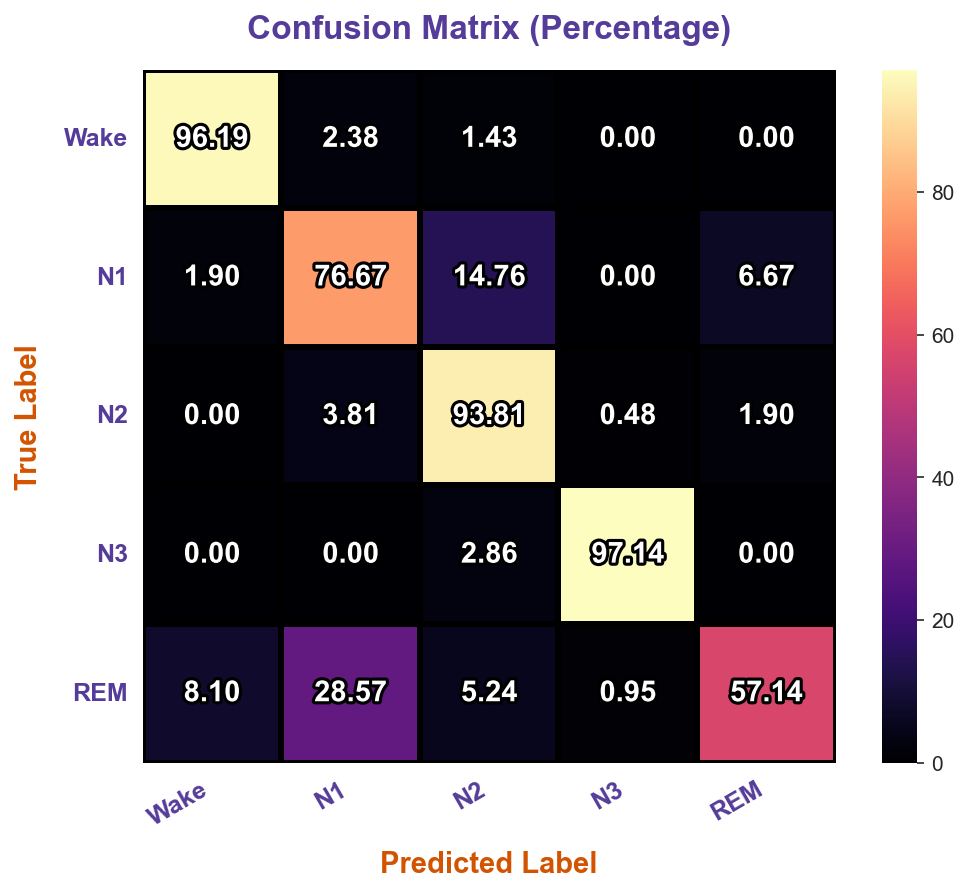
\includegraphics[width=\linewidth]{img/paper_3/confusion matrix percentatge wise}
		\caption{Confusion matrix (percentage)}
		\label{fig:confusion-matrix-percentatge-wise}
	\end{minipage}
	\hfill
	\begin{minipage}[b]{0.45\linewidth}
		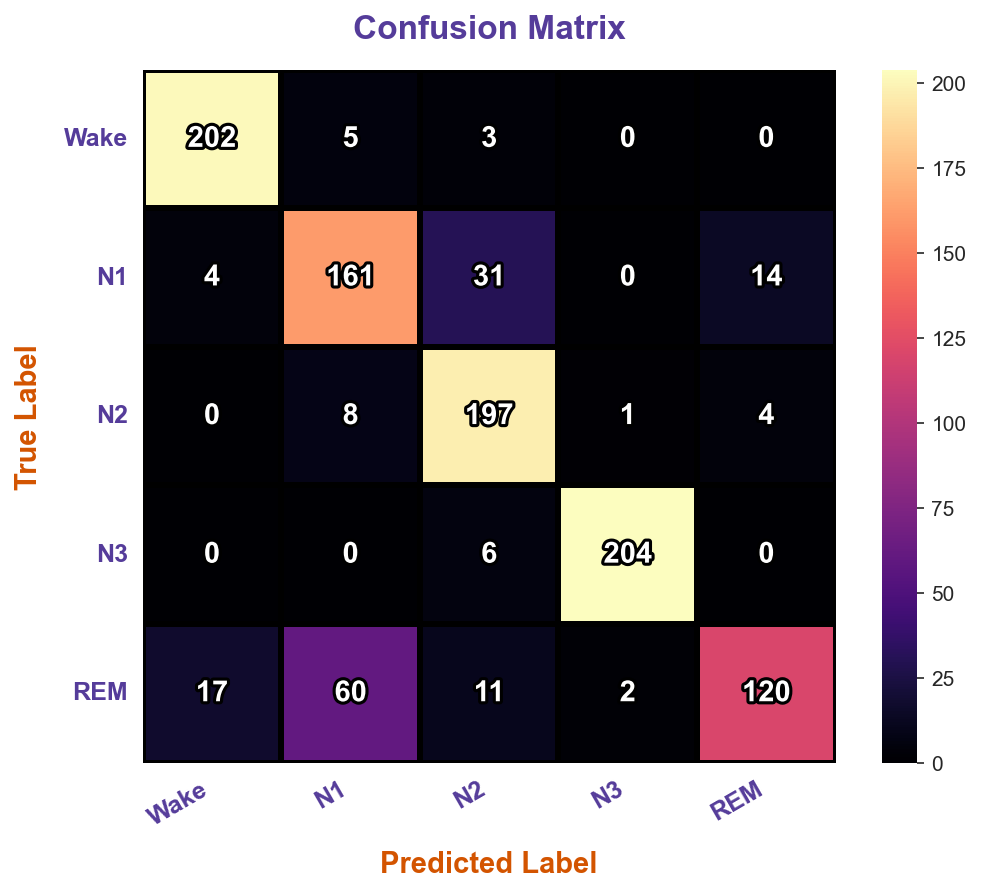
\includegraphics[width=\linewidth]{img/paper_3/confusion matrix samples}
		\caption{Confusion matrix (samples)}
		\label{fig:confusion-matrix-samples}
	\end{minipage}
\end{figure}

\begin{figure}[htbp]
	\centering
	\begin{minipage}[b]{0.45\linewidth}
		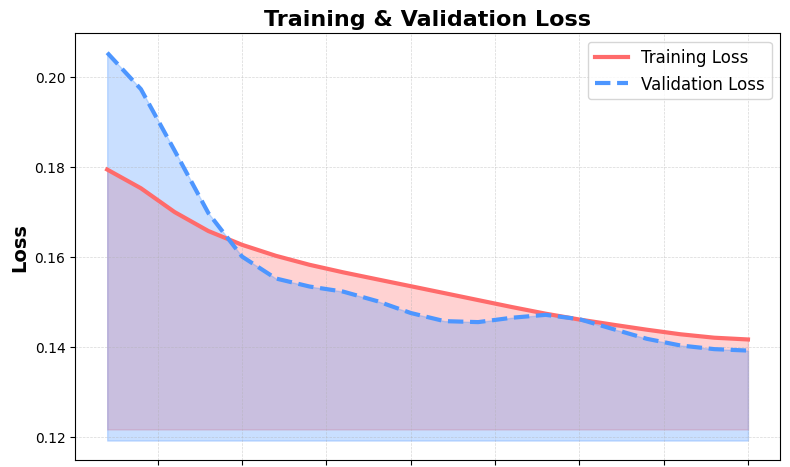
\includegraphics[width=\linewidth]{img/paper_3/loss plot}
		\caption{Loss plot}
		\label{fig:loss-plot}
	\end{minipage}
	\hfill
	\begin{minipage}[b]{0.45\linewidth}
		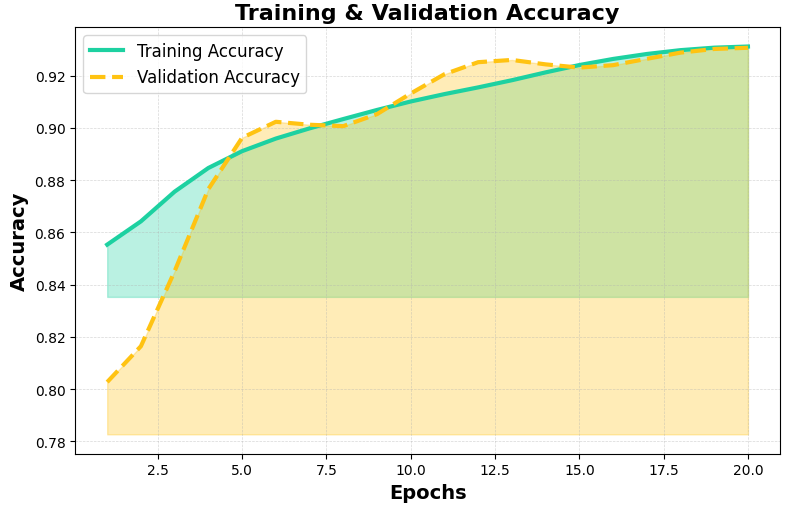
\includegraphics[width=\linewidth]{img/paper_3/accuracy plot}
		\caption{Accuracy plot}
		\label{fig:accuracy-plot}
	\end{minipage}
\end{figure}

The class weight distribution used during training is as follows: 0: 1.1923, 1: 5.8152, 2: 2.4719, 3: 4.8223, 4: 4.0506. These values reflect adjustments to counter class imbalance and ensure fairer learning across all sleep stages.

The progression of model performance across selected epochs is summarized below:

\begin{figure}[htbp]
	\centering
	\begin{minipage}[b]{0.45\linewidth}
		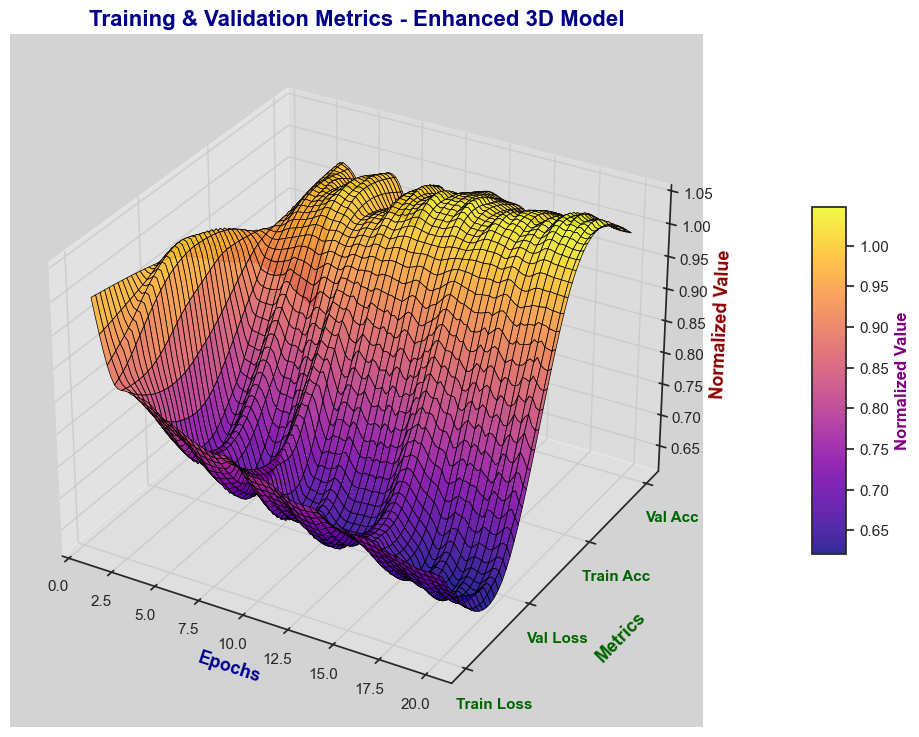
\includegraphics[width=\linewidth]{img/paper_3/3D acc loss plot}
		\caption{3D Accuracy vs. Loss}
		\label{fig:3d-acc-loss-plot}
	\end{minipage}
\end{figure}


The sample distribution plot reveals a nearly normal distribution of data across the various sleep stages, confirming a balanced dataset. For the test phase, approximately 1,050 samples were utilized, with 210 samples assigned to each class, ensuring equitable and unbiased performance evaluation.

\begin{figure}[htbp]
	\centering
	\begin{minipage}[b]{0.45\linewidth}
		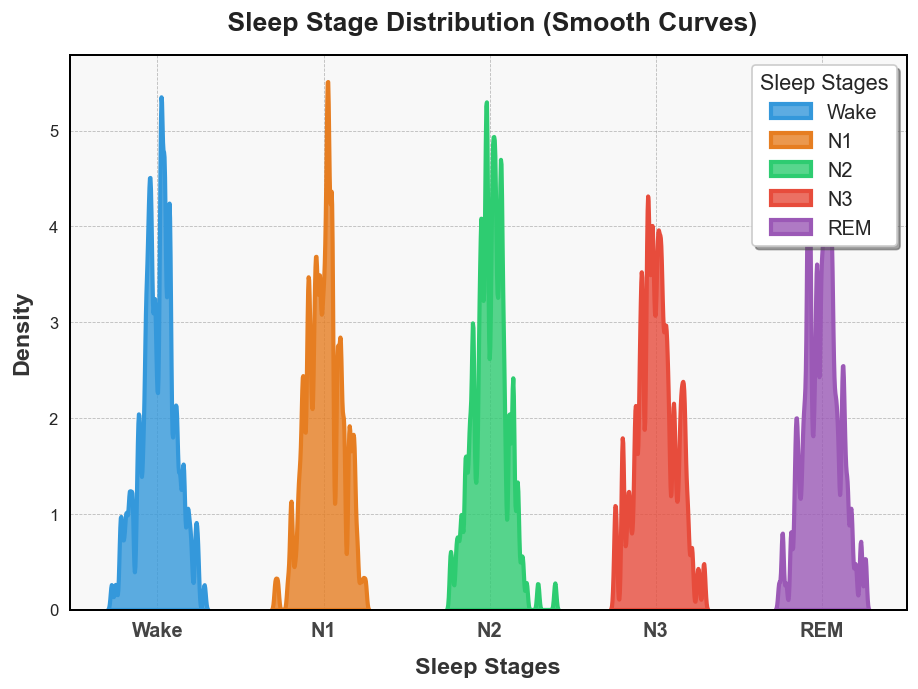
\includegraphics[width=\linewidth]{img/paper_3/sample distribution plot pdf}
		\caption{Sample distribution}
		\label{fig:sample-distribution-plot-pdf}
	\end{minipage}
	\hfill
	\begin{minipage}[b]{0.45\linewidth}
		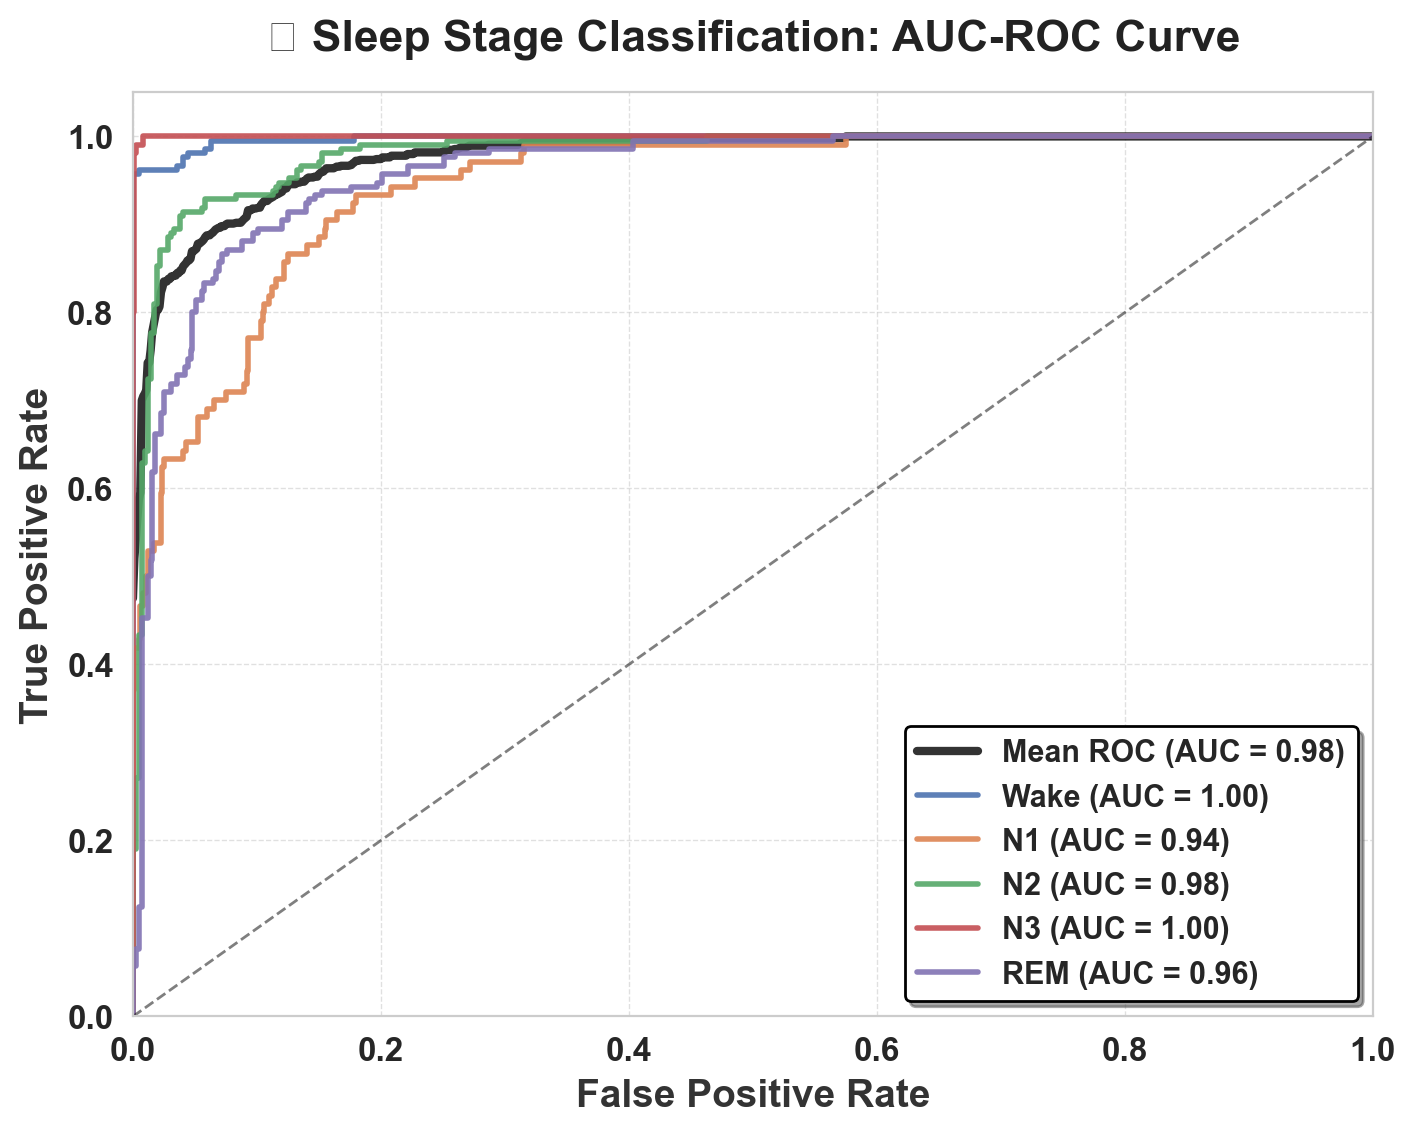
\includegraphics[width=\linewidth]{img/paper_3/auc vs roc curve}
		\caption{AUC vs. ROC Curve}
		\label{fig:auc-vs-roc-curve}
	\end{minipage}
\end{figure}

\begin{figure}[htbp]
	\centering
	\begin{minipage}[b]{0.31\linewidth}
		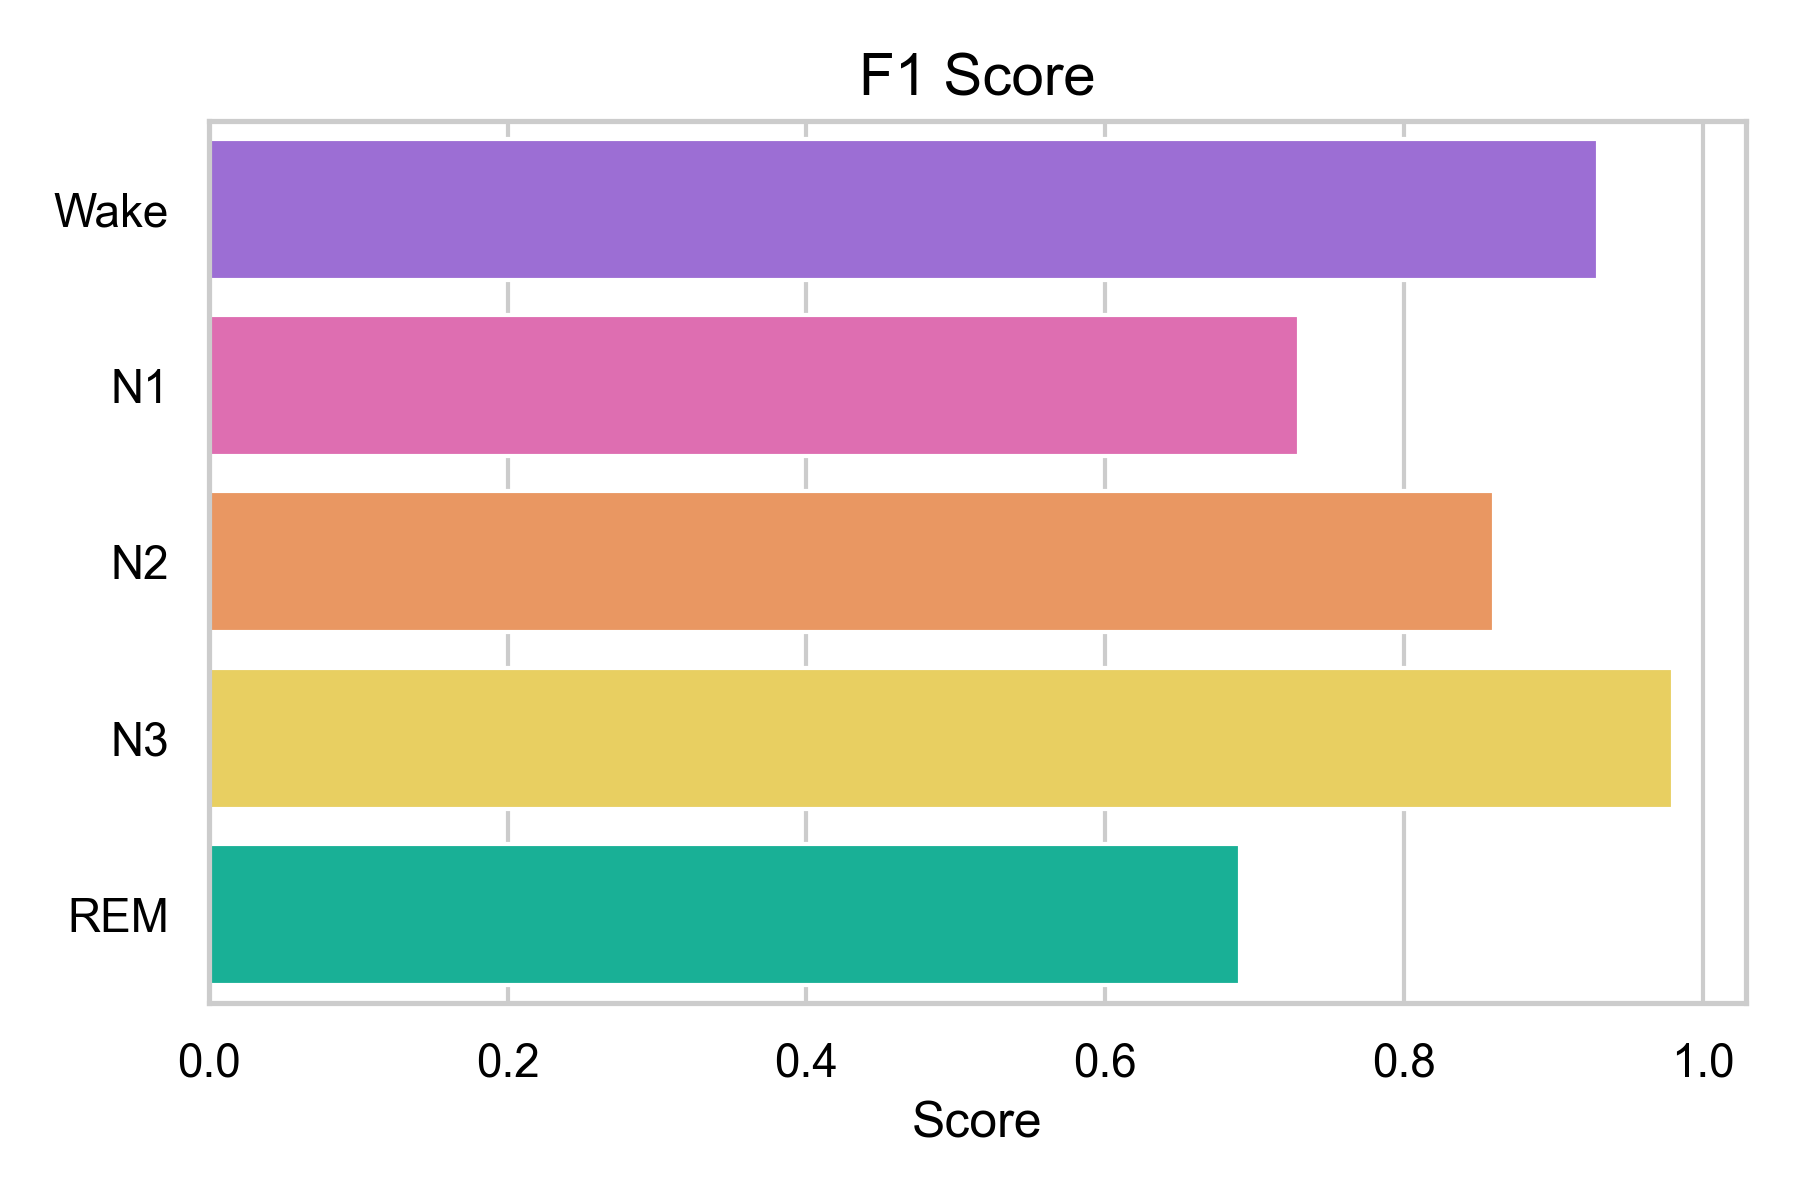
\includegraphics[width=\linewidth]{img/paper_3/f1_score_plot}
		\caption{F1 Score}
		\label{fig:f1scoreplot}
	\end{minipage}
	\hfill
	\begin{minipage}[b]{0.31\linewidth}
		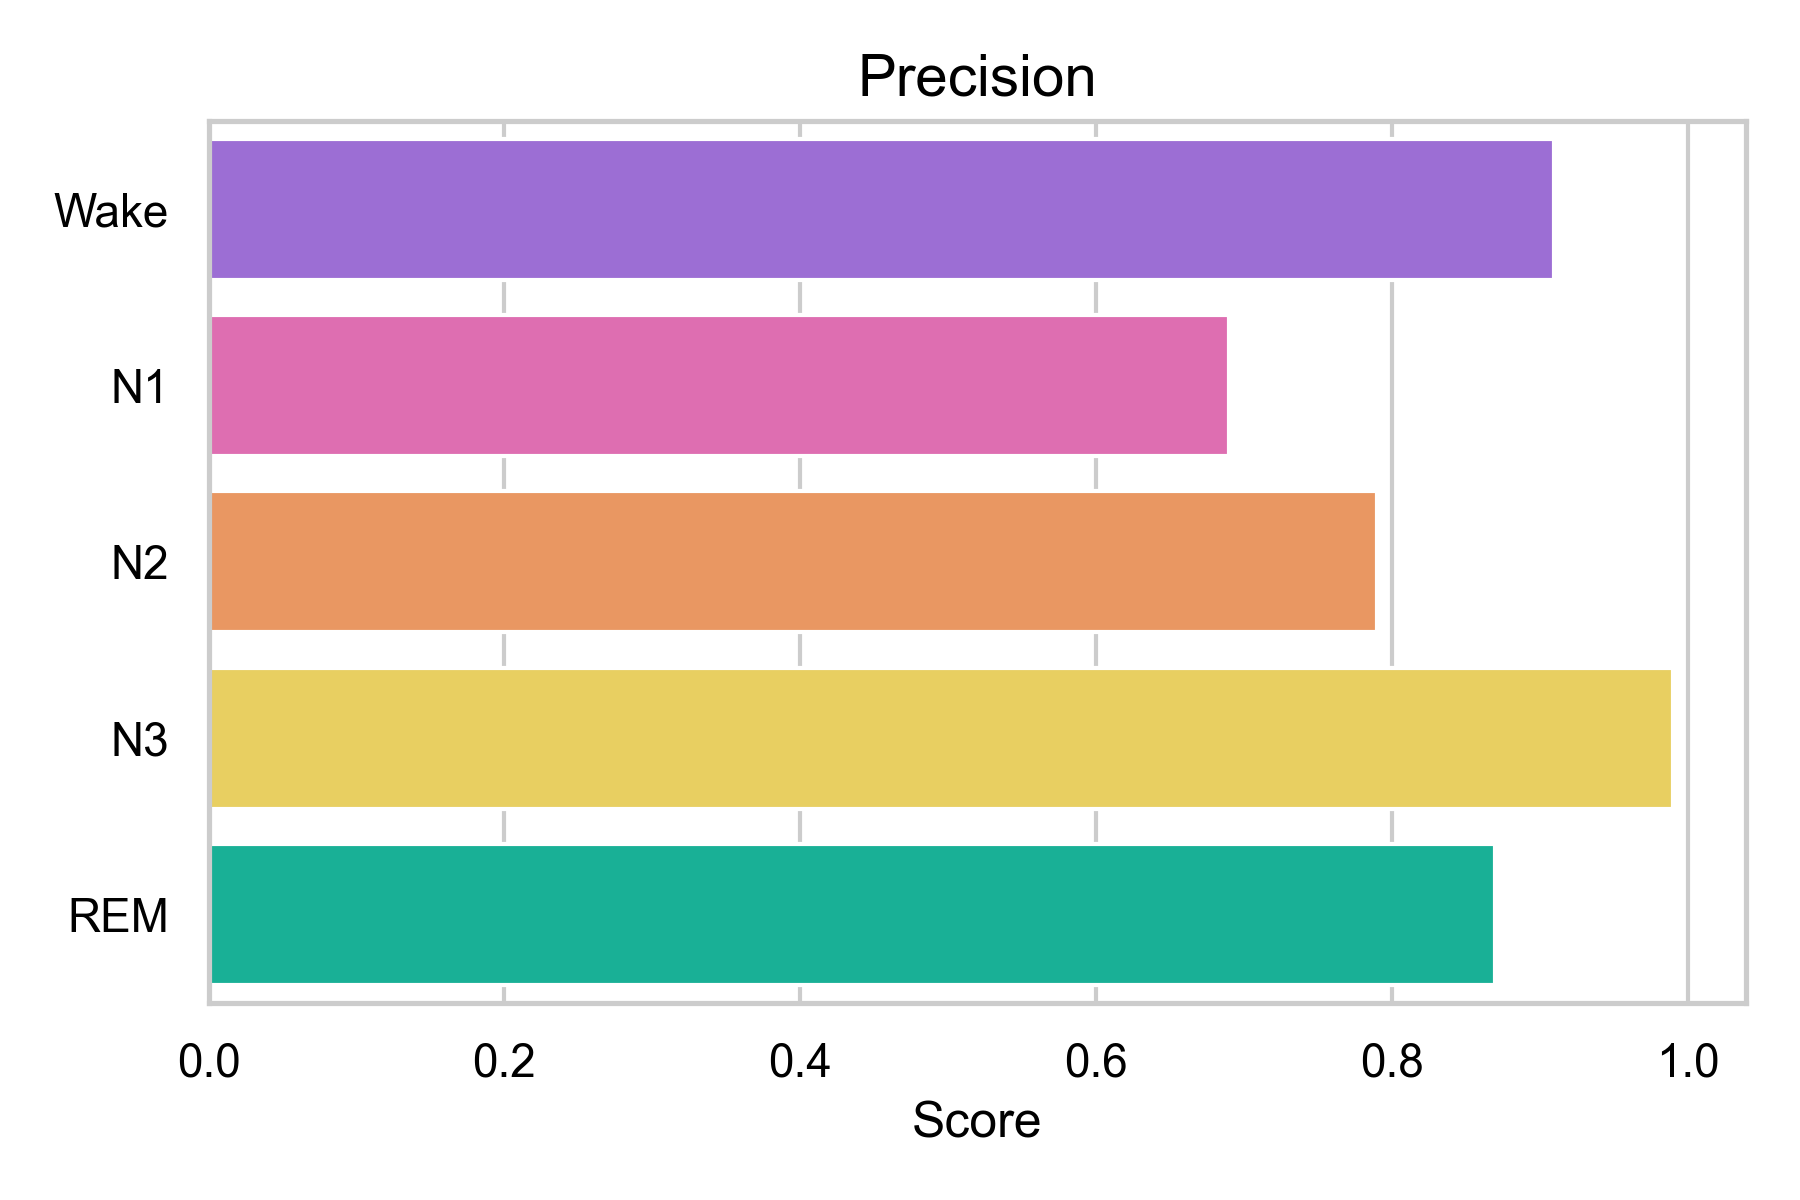
\includegraphics[width=\linewidth]{img/paper_3/precision_plot}
		\caption{Precision}
		\label{fig:precisionplot}
	\end{minipage}
	\hfill
	\begin{minipage}[b]{0.31\linewidth}
		\includegraphics[width=\linewidth]{img/paper_3/recall_plot}
		\caption{Recall}
		\label{fig:recallplot}
	\end{minipage}
\end{figure}















\subsection{XAI Visualization with Heatmap and Plots}





This section presents the distribution of sleep stage data, which approximates a normal distribution. The dataset is well-balanced, with an equal number of samples across all sleep stages. For testing purposes, approximately 1,050 samples were selected, ensuring that each sleep stage class contains around 210 samples. This balanced distribution supports a fair and unbiased evaluation of the model's performance.





\begin{figure}[H]
	\centering
	\includegraphics[width=0.7\linewidth]{"img/paper_3/shap important"}
	\caption{Bar plot illustrating EEG channel importance based on SHAP values. Higher SHAP values indicate greater influence on the model's sleep stage predictions.}
	
	\label{fig:shap-important}
\end{figure}




\subsubsection*{Interpretable Sleep Stage Classification: Hypnogram Transitions and Feature Importance using LIME and SHAP}

\begin{figure}[H]
	\centering
	\begin{minipage}[b]{0.45\linewidth}
		\includegraphics[width=\linewidth]{"img/paper_3/stage n1"}
		\caption{Stage N1}
		\label{fig:stage-n1}
	\end{minipage}
	\hfill
	\begin{minipage}[b]{0.45\linewidth}
		\includegraphics[width=\linewidth]{"img/paper_3/stage n2"}
		\caption{Stage N2}
		\label{fig:stage-n2}
	\end{minipage}
\end{figure}




To improve the interpretability of the sleep stage classification model, we employ Explainable AI (XAI) techniques. Initially, we analyze the hypnogram transition plot, which illustrates the temporal sequence of sleep stages. This visualization helps assess whether the model's predictions align with the natural and expected progression of sleep cycles.


\begin{figure}[htbp]
	\centering
	\begin{minipage}[b]{0.45\linewidth}
		\includegraphics[width=\linewidth]{"img/paper_3/stage n3"}
		\caption{Stage N3}
		\label{fig:stage-n3}
	\end{minipage}
	\hfill
	\begin{minipage}[b]{0.45\linewidth}
		\includegraphics[width=\linewidth]{"img/paper_3/stage rem"}
		\caption{Stage REM}
		\label{fig:stage-rem}
	\end{minipage}
\end{figure}



Subsequently, we utilize LIME (Local Interpretable Model-Agnostic Explanations) and SHAP (SHapley Additive exPlanations) to investigate feature importance. These tools provide both global and local explanations of the model's behavior. Specifically, they identify the EEG channels that significantly influence the model's decisions, offering insight into which features are most critical in sleep stage classification.




\begin{figure}[htbp]
	\centering
	\begin{minipage}[b]{0.45\linewidth}
		\includegraphics[width=\linewidth]{"img/paper_3/stage wake"}
		\caption{Stage Wake}
		\label{fig:stage-wake}
	\end{minipage}
	\hfill
	\begin{minipage}[b]{0.45\linewidth}
		\includegraphics[width=\linewidth]{img/paper_3/XAI4}
		\caption{XAI Visualization}
		\label{fig:xai4}
	\end{minipage}
\end{figure}


By leveraging these interpretability techniques, we ensure that the model's predictions are not only accurate but also aligned with known physiological sleep dynamics, thereby enhancing trust and transparency in the model's outcomes.









































\subsection{Time Complexity Analysis}

\begin{figure}[H]
	\centering
	\begin{minipage}[b]{0.40\linewidth}
		\centering
		\includegraphics[width=\linewidth]{img/paper_3/preprocessing_on³}
		\caption{Preprocessing (\(O(MN^3 + KEN + MN)\))}
		\label{fig:preprocessingon3}
	\end{minipage}
	\hfill
	\begin{minipage}[b]{0.40\linewidth}
		\centering
		\includegraphics[width=\linewidth]{img/paper_3/training_loop_ot·…}
		\caption{Training Loop (\(O(T(LN + 2N^2D/10^4 + DC))\))}
		\label{fig:trainingloopot}
	\end{minipage}
\end{figure}

\noindent Preprocessing: \(O(MN^3 + KEN + MN)\) \\
Training Loop: \(O(T(LN + 2N^2D/10^4 + DC))\)

\begin{figure}[H]
	\centering
	\begin{minipage}[b]{0.40\linewidth}
		\centering
		\includegraphics[width=\linewidth]{img/paper_3/gcn_layers_on}
		\caption{GCN Layers (\(O(LN)\))}
		\label{fig:gcnlayerson}
	\end{minipage}
	\hfill
	\begin{minipage}[b]{0.40\linewidth}
		\centering
		\includegraphics[width=\linewidth]{img/paper_3/transformer_encoder_on²}
		\caption{Transformer Encoder (\(O(N^2D)\))}
		\label{fig:transformerencoderon2}
	\end{minipage}
\end{figure}

\noindent GCN Layers: \(O(LN)\) \\
Transformer Encoder: \(O(N^2D)\)

\begin{figure}[H]
	\centering
	\begin{minipage}[b]{0.40\linewidth}
		\centering
		\includegraphics[width=\linewidth]{img/paper_3/evaluation_oe_val·…}
		\caption{Evaluation Loop (\(O(E_{\text{val}}(LN + 2N^2D/10^4 + DC))\))}
		\label{fig:evaluationoeval}
	\end{minipage}
	\hfill
	\begin{minipage}[b]{0.40\linewidth}
		\centering
		\includegraphics[width=\linewidth]{img/paper_3/fully_connected_layer_o1}
		\caption{Fully Connected Layer (\(O(DC)\))}
		\label{fig:fullyconnectedlayero1}
	\end{minipage}
\end{figure}

\noindent Evaluation Loop: \(O(E_{\text{val}}(LN + 2N^2D/10^4 + DC))\) \\
Fully Connected Layer: \(O(DC)\)

\chapter{Discussion}
\label{chapter_discussion}
\pagestyle{plain}



\subsection{Principal Contributions}
This study proposes a novel graph-based representation for sleep EEG data, integrating a hybrid GCN-Transformer architecture to improve the classification of sleep stages. By effectively capturing both spatial and temporal dependencies, our model outperforms traditional deep learning approaches in terms of accuracy and robustness. The incorporation of graph structures, combined with attention mechanisms, facilitates a more nuanced understanding of sleep dynamics.

\subsection{Distinctive Aspects of Our Approach}
Conventional methods such as CNNs primarily emphasize spatial features, whereas RNNs address temporal dynamics but are limited in handling long-range dependencies. Our model bridges this gap by combining the spatial modeling capabilities of Graph Convolutional Networks (GCNs) with the sequence modeling strengths of Transformers. Moreover, the use of Focal Loss and Label Smoothing addresses class imbalance effectively. The explainability component of our framework, supported by XAI techniques, identifies key EEG channels that influence sleep stage transitions, enhancing interpretability and clinical relevance.

\subsection{Performance Highlights}
Several components contribute to the model’s success. The graph-based representation enables the retention of spatial relationships across EEG nodes, promoting more effective learning of brain activity patterns. The fusion of GCN and Transformer modules allows the network to model complex spatial-temporal interactions, yielding highly accurate sleep stage predictions. Techniques for mitigating class imbalance—such as Focal Loss and Label Smoothing—enhance reliability, especially in underrepresented stages. Additionally, explainability features provide actionable insights into the neural correlates of sleep, supporting broader medical and neuroscientific applications.

\subsection{Limitations and Future Directions}
Despite its strengths, the proposed method has notable limitations. The combined GCN-Transformer model incurs higher computational costs compared to lighter architectures like CNNs or LSTMs, which may restrict deployment in resource-constrained environments. The Sleep-EDF dataset, although widely used, includes a limited sample of subjects, potentially affecting generalizability. Furthermore, while acceleration via Apple M1 and Metal APIs improves efficiency, larger models would benefit from more powerful hardware such as GPUs or TPUs. 


\chapter{Conclusion}
\label{chapter_conclusion}
\pagestyle{plain}
\section{Discussion}

\subsection{Principal Contributions}
This study proposes a novel graph-based representation for sleep EEG data, integrating a hybrid GCN-Transformer architecture to improve the classification of sleep stages. By effectively capturing both spatial and temporal dependencies, our model outperforms traditional deep learning approaches in terms of accuracy and robustness. The incorporation of graph structures, combined with attention mechanisms, facilitates a more nuanced understanding of sleep dynamics.

\subsection{Distinctive Aspects of Our Approach}
Conventional methods such as CNNs primarily emphasize spatial features, whereas RNNs address temporal dynamics but are limited in handling long-range dependencies. Our model bridges this gap by combining the spatial modeling capabilities of Graph Convolutional Networks (GCNs) with the sequence modeling strengths of Transformers. Moreover, the use of Focal Loss and Label Smoothing addresses class imbalance effectively. The explainability component of our framework, supported by XAI techniques, identifies key EEG channels that influence sleep stage transitions, enhancing interpretability and clinical relevance.

\subsection{Performance Highlights}
Several components contribute to the model’s success. The graph-based representation enables the retention of spatial relationships across EEG nodes, promoting more effective learning of brain activity patterns. The fusion of GCN and Transformer modules allows the network to model complex spatial-temporal interactions, yielding highly accurate sleep stage predictions. Techniques for mitigating class imbalance—such as Focal Loss and Label Smoothing—enhance reliability, especially in underrepresented stages. Additionally, explainability features provide actionable insights into the neural correlates of sleep, supporting broader medical and neuroscientific applications.

\subsection{Limitations and Future Directions}
Despite its strengths, the proposed method has notable limitations. The combined GCN-Transformer model incurs higher computational costs compared to lighter architectures like CNNs or LSTMs, which may restrict deployment in resource-constrained environments. The Sleep-EDF dataset, although widely used, includes a limited sample of subjects, potentially affecting generalizability. Furthermore, while acceleration via Apple M1 and Metal APIs improves efficiency, larger models would benefit from more powerful hardware such as GPUs or TPUs. Future work may explore more scalable architectures and validate the approach on larger, more diverse datasets.

\section{Conclusion}

The proposed SleepGCN-Transformer architecture demonstrates superior performance in sleep stage classification, achieving 93.12\% training accuracy and 93.04\% validation accuracy. By integrating GCNs to model spatial interdependencies and Transformers to extract temporal patterns, the model effectively captures the complexity of sleep physiology. The application of Focal Loss contributes to robust handling of class imbalance, improving classification across all stages. Feature importance analysis indicates that EMG and the EEG Pz-Oz channel play a critical role in prediction. This approach not only improves predictive performance but also enhances interpretability, laying a foundation for future work in explainable and clinically applicable sleep analysis tools.




\chapter{Appendix: Resources and Dataset Information}
\label{chapter_appendix}
\begin{figure}[h!]
	\centering
	\begin{minipage}[b]{0.3\linewidth}
		\centering
		\includegraphics[width=\linewidth]{img/paper3}
		\caption{Automated Sleep Staging System with EEG Signal using Machine Learning Techniques}
		\label{fig:paper3}
	\end{minipage}\hfill
	\begin{minipage}[b]{0.3\linewidth}
		\centering
		\includegraphics[width=\linewidth]{img/paper1}
		\caption{Deep Neural Model for Automated Sleep Staging System using Single-Channel EEG Signal}
		\label{fig:paper1}
	\end{minipage}\hfill
	\begin{minipage}[b]{0.3\linewidth}
		\centering
		\includegraphics[width=\linewidth]{img/paper2}
		\caption{SleepGCN-Transformer: A Hybrid Graph-Convolutional and Transformer Network for Sleep Stage Classification}
		\label{fig:paper2}
	\end{minipage}
\end{figure}

\section{1. Dataset}
We conducted our experiments using the \textbf{Sleep-EDF dataset}, a publicly available dataset for sleep analysis research.\\
\texttt{https://physionet.org/content/sleep-edfx/1.0.0/}

\section{2. Development Environment}
Our implementation was carried out using the following configurations:
\begin{itemize}
	\item \textbf{Programming Language}: Python 3.13.1
	\item \textbf{Deep Learning Framework}: PyTorch
	\item \textbf{IDE}: VS Code
	\item \textbf{Hardware}: Apple M1 Chip (CPU and Metal for acceleration)
\end{itemize}

\section{3. Version Control}
To manage our codebase, we used GitHub for version control.\\
QR code available alongside the figures.

\section{4. License}
The source code of this research is registered under the \textbf{Apache License 2.0}.\\
\texttt{http://www.apache.org/licenses/}

\section{5. Key Python Libraries \& Versions}
\begin{itemize}
	\item \textbf{NumPy}: 2.2.2
	\item \textbf{Pandas}: 2.2.3
	\item \textbf{Scikit-learn}: 1.6.1
	\item \textbf{SciPy}: 1.15.1
	\item \textbf{Matplotlib}: 3.10.0
	\item \textbf{Seaborn}: 0.13.2
	\item \textbf{PyTorch}: 2.6.0
	\item \textbf{Torch Geometric}: 2.6.1
	\item \textbf{NetworkX}: 3.4.2
	\item \textbf{MNE}: 1.9.0
\end{itemize}
This setup ensures a robust and reproducible environment for the development and evaluation of our sleep stage classification model.


\chapter{References}
\label{chapter_references}
\begin{thebibliography}{99}
	
	\bibitem{han2024classification}
	H.~Han et~al., ``Classification and automatic scoring of arousal intensity during sleep stages using machine learning,'' \emph{Scientific Reports}, vol.~14, no.~1, Dec. 2024, doi: \href{https://doi.org/10.1038/s41598-023-50653-9}{10.1038/s41598-023-50653-9}.
	
	\bibitem{tsinalis2016automatic}
	O.~Tsinalis et~al., ``Automatic Sleep Stage Scoring Using Time-Frequency Analysis and Stacked Sparse Autoencoders,'' \emph{Annals of Biomedical Engineering}, vol.~44, no.~5, May 2016, doi: \href{https://doi.org/10.1007/s10439-015-1444-y}{10.1007/s10439-015-1444-y}.
	
	\bibitem{krakovska2011automatic}
	A.~Krakovská and K.~Mezeiová, ``Automatic sleep scoring: A search for an optimal combination of measures,'' \emph{Artificial Intelligence in Medicine}, vol.~53, no.~1, Sep. 2011, doi: \href{https://doi.org/10.1016/j.artmed.2011.06.004}{10.1016/j.artmed.2011.06.004}.
	
	\bibitem{biswal2018expert}
	S.~Biswal et~al., ``Expert-level sleep scoring with deep neural networks,'' \emph{Journal of the American Medical Informatics Association}, vol.~25, no.~12, Dec. 2018, doi: \href{https://doi.org/10.1093/jamia/ocy131}{10.1093/jamia/ocy131}.
	
	\bibitem{ronzhina2012sleep}
	M.~Ronzhina et~al., ``Sleep scoring using artificial neural networks,'' \emph{Sleep Medicine Reviews}, vol.~16, no.~3, Jun. 2012, doi: \href{https://doi.org/10.1016/j.smrv.2011.06.003}{10.1016/j.smrv.2011.06.003}.
	
	\bibitem{alsolai2022systematic}
	H.~Alsolai et~al., ``A Systematic Review of Literature on Automated Sleep Scoring,'' \emph{IEEE Access}, vol.~10, pp.~79419--79443, 2022, doi: \href{https://doi.org/10.1109/ACCESS.2022.3194145}{10.1109/ACCESS.2022.3194145}.
	
	\bibitem{fiorillo2019automated}
	L.~Fiorillo et~al., ``Automated sleep scoring: A review of the latest approaches,'' \emph{Sleep Medicine Reviews}, vol.~48, Dec. 2019, doi: \href{https://doi.org/10.1016/j.smrv.2019.07.007}{10.1016/j.smrv.2019.07.007}.
	
	\bibitem{faust2019review}
	O.~Faust et~al., ``A review of automated sleep stage scoring based on physiological signals for the new millennia,'' \emph{Computer Methods and Programs in Biomedicine}, vol.~176, Jul. 2019, doi: \href{https://doi.org/10.1016/j.cmpb.2019.04.032}{10.1016/j.cmpb.2019.04.032}.
	
	\bibitem{chriskos2021review}
	P.~Chriskos et~al., ``A review on current trends in automatic sleep staging through bio-signal recordings and future challenges,'' \emph{Sleep Medicine Reviews}, vol.~55, Feb. 2021, doi: \href{https://doi.org/10.1016/j.smrv.2020.101377}{10.1016/j.smrv.2020.101377}.
	
	\bibitem{phan2022sleeptransformer}
	H.~Phan, K.~B. Mikkelsen, O.~Y. Chen, P.~Koch, A.~Mertins, and M.~De~Vos, ``SleepTransformer: Automatic Sleep Staging with Interpretability and Uncertainty Quantification,'' \emph{IEEE Transactions on Biomedical Engineering}, 2022.
	
	

	
	\bibitem{han2024classification}
	H.~Han et~al., ``Classification and automatic scoring of arousal intensity during sleep stages using machine learning,'' \emph{Scientific Reports}, vol.~14, no.~1, Dec. 2024.
	
	\bibitem{tsinalis2016automatic}
	O.~Tsinalis et~al., ``Automatic Sleep Stage Scoring Using Time-Frequency Analysis and Stacked Sparse Autoencoders,'' \emph{Annals of Biomedical Engineering}, vol.~44, no.~5, May 2016.
	
	\bibitem{krakovska2011automatic}
	A.~Krakovská and K.~Mezeiová, ``Automatic sleep scoring: A search for an optimal combination of measures,'' \emph{Artificial Intelligence in Medicine}, vol.~53, no.~1, Sep. 2011.
	
	\bibitem{biswal2018expert}
	S.~Biswal et~al., ``Expert-level sleep scoring with deep neural networks,'' \emph{JAMIA}, vol.~25, no.~12, Dec. 2018.
	
	\bibitem{ronzhina2012sleep}
	M.~Ronzhina et~al., ``Sleep scoring using artificial neural networks,'' \emph{Sleep Medicine Reviews}, vol.~16, no.~3, Jun. 2012.
	
	\bibitem{alsolai2022systematic}
	H.~Alsolai et~al., ``A Systematic Review of Literature on Automated Sleep Scoring,'' \emph{IEEE Access}, vol.~10, 2022.
	
	\bibitem{fiorillo2019automated}
	L.~Fiorillo et~al., ``Automated sleep scoring: A review of the latest approaches,'' \emph{Sleep Medicine Reviews}, vol.~48, Dec. 2019.
	
	\bibitem{faust2019review}
	O.~Faust et~al., ``A review of automated sleep stage scoring based on physiological signals for the new millennia,'' \emph{Computer Methods and Programs in Biomedicine}, vol.~176, Jul. 2019.
	
	\bibitem{chriskos2021review}
	P.~Chriskos et~al., ``A review on current trends in automatic sleep staging through bio-signal recordings and future challenges,'' \emph{Sleep Medicine Reviews}, vol.~55, Feb. 2021.
	
	\bibitem{phan2022sleeptransformer}
	H.~Phan et~al., ``SleepTransformer: Automatic Sleep Staging with Interpretability and Uncertainty Quantification,'' \emph{IEEE Transactions on Biomedical Engineering}, 2022.
	
	\bibitem{dai2023multichannelsleepnet}
	Y.~Dai et~al., ``MultiChannelSleepNet: A Transformer-Based Model for Automatic Sleep Stage Classification With PSG,'' \emph{IEEE J. Biomed. Health Inform.}, 2023.
	
	\bibitem{guo2024flexsleeptransformer}
	Y.~Guo, M.~Nowakowski, and W.~Dai, ``FlexSleepTransformer: A Transformer-Based Sleep Staging Model with Flexible Input Channel Configurations,'' \emph{Scientific Reports}, 2024.
	
	\bibitem{yao2022cnntransformer}
	Z.~Yao and X.~Liu, ``A CNN-Transformer Deep Learning Model for Real-time Sleep Stage Classification in an Energy-Constrained Wireless Device,'' \emph{medRxiv}, 2022.
	
	\bibitem{supratak2017deepsleepnet}
	A.~Supratak et~al., ``DeepSleepNet: A Model for Automatic Sleep Stage Scoring Based on Raw Single-Channel EEG,'' \emph{IEEE Trans. Neural Syst. Rehabil. Eng.}, vol.~25, no.~11, pp.~1998--2008, 2017.
	
	\bibitem{eldele2021attnsleep}
	E.~Eldele et~al., ``AttnSleep: An Attention-Based Deep Learning Approach for Sleep Stage Classification With Single-Channel EEG,'' \emph{IEEE Trans. Neural Syst. Rehabil. Eng.}, 2021.
	
	\bibitem{ji2022jkstgcn}
	X.~Ji, Y.~Li, and P.~Wen, ``Jumping Knowledge-Based Spatial-Temporal Graph Convolutional Networks for Automatic Sleep Stage Classification,'' \emph{IEEE Trans. Neural Syst. Rehabil. Eng.}, 2022.
	
	\bibitem{mousavi2019sleepeegnet}
	S.~Mousavi, F.~Afghah, and U.~R. Acharya, ``SleepEEGNet: Automated Sleep Stage Scoring With Sequence-to-Sequence Deep Learning Approach,'' \emph{PLOS ONE}, 2019.
	
	\bibitem{phan2019seqsleepnet}
	H.~Phan et~al., ``SeqSleepNet: End-to-End Hierarchical Recurrent Neural Network for Sequence-to-Sequence Automatic Sleep Staging,'' \emph{IEEE Trans. Neural Syst. Rehabil. Eng.}, 2019.
	
	\bibitem{zhang2024cnntransformerconvlstm}
	Zhang et~al., ``A CNN-Transformer-ConvLSTM-CRF Hybrid Network for Sleep Stage Classification,'' \emph{IEEE Sensors Journal}, 2024.
	
	\bibitem{liu2024review}
	Liu et~al., ``Automatic Sleep Stage Classification Using Deep Learning: Signals, Data Representation, and Neural Networks,'' \emph{Artificial Intelligence Review}, 2024.
	
	\bibitem{ctdal2022}
	CT-DAL, ``Convolutional Transformer with Domain Adversarial Learning for Multi-Channel Sleep Stage Classification,'' \emph{Available on Semantic Scholar}, 2022.
	
	\bibitem{pei2022hybrid}
	W.~Pei, Y.~Li, S.~Siuly, and P.~Wen, ``A Hybrid Deep Learning Scheme for Multi-Channel Sleep Stage Classification,'' \emph{Computers, Materials \& Continua}, 2022.
	
	\bibitem{mostafaei2024crossmodality}
	S.~H. Mostafaei, J.~Tanha, and A.~Sharafkhaneh, ``A Novel Deep Learning Model Based on Transformer and Cross-Modality Attention for Classification of Sleep Stages,'' \emph{Journal of Biomedical Informatics}, 2024.
	
	\bibitem{jeong2024explainablevit}
	Jeong et~al., ``Explainable Vision Transformer for Automatic Visual Sleep Staging,'' \emph{npj Digital Medicine}, 2024.
	
	\bibitem{pei2024mfcc}
	W.~Pei, Y.~Li et~al., ``An Automatic Method Using MFCC Features for Sleep Stage Classification,'' \emph{Biomedical Signal Processing and Control}, 2024.
	
	\bibitem{sors2018cnn}
	A.~Sors et~al., ``A Convolutional Neural Network for Sleep Stage Scoring from Raw Single-Channel EEG,'' \emph{Biomedical Signal Processing and Control}, 2018.
	
	\bibitem{seo2020iitnet}
	H.~Seo et~al., ``Intra- and Inter-Epoch Temporal Context Network (IITNet) Using Sub-Epoch Features for Automatic Sleep Scoring on Raw Single-Channel EEG,'' \emph{Biomedical Signal Processing and Control}, 2020.
	
	\bibitem{biswal2017sleepnet}
	S.~Biswal et~al., ``SLEEPNET: Automated Sleep Staging System via Deep Learning,'' \emph{Journal of the American Medical Informatics Association}, 2017.
	
	\bibitem{phan2018jointcnn}
	H.~Phan et~al., ``Joint Classification and Prediction CNN Framework for Automatic Sleep Stage Classification,'' \emph{IEEE Transactions on Biomedical Engineering}, 2018.
	
\end{thebibliography}



\clearpage
\thispagestyle{empty}

\end{document}
